\documentclass{article}

\usepackage{amsmath,amsfonts,unicode-math,amsthm,enumitem}
\usepackage{pdfpages}
\usepackage[a4paper]{geometry}
\usepackage{float}
\usepackage{subfigure}
%\setmathfont{Asana Math}
%\setmathfont{XITS Math}
%\setmathfont{STIX Math}

\theoremstyle{plain}
\newtheorem*{theo}{Theorem}
\theoremstyle{definition}
\newtheorem*{defi}{Definition}
\newtheorem*{exa}{Example}
\newtheorem*{lem}{Lemma}
\newtheorem*{cor}{Corollary}
\newtheorem*{pro}{Proposition}
\theoremstyle{remark}
\newtheorem*{rem}{Remark}

\setenumerate[0]{label=(\roman*)}

\newcommand\md{\mathop{}\!\mathrm{d}}
\newcommand\dist{\mathop{}\mathrm{d}}
\newcommand\diam{\mathop{}\mathrm{diam}}
\newcommand\avg{\mathrm{avg}}
\newcommand\Leb{\mathrm{Leb}}
\newcommand\Lip{\mathrm{Lip}}
\newcommand\Disc{\mathrm{Disc}}
\newcommand\Ba{\mathcal{B}}
\newcommand\BV{\mathrm{BV}}
\newcommand\AC{\mathrm{AC}}
\newcommand\hm{\mathcal{H}}
\newcommand\C{\mathcal{C}}
\newcommand\R{\mathcal{R}}
\newcommand\loc{\mathrm{loc}}
\newcommand\highl[1]{\textit{#1}}


\graphicspath{ {../img/} }
\begin{document}

\title{Geometric Aspects of Harmonic Analysis}
\author{Dr Diogo Oliveira e Silva}
\maketitle
\paragraph{Q1}
\begin{equation*}
	\left.
		\begin{matrix}
			f:[a,b]→ℝ\text{ integrable}\\
			F(x)=∫_a^xf(t)\md t
		\end{matrix}
	\right]\underset?⇒ F\text{ diff. (a.e. $x$)},\ F'=f
\end{equation*}
\paragraph{Q2} Conditions of $F$ (on $[a,b]$) s.t. 
\begin{itemize}
	\item $F'(x)$ exists a.e.
	\item $F'$ integrable
	\item $∫_a^bF'(x)\md x=F(b)-F(a)$
\end{itemize} ?
\paragraph{Q1} Differentiation of the integral
\begin{equation*}
	\frac{F(x+h)-F(x)}h=\frac1h∫_x^{x+h}f(t)\md t=\frac1{|I|}∫f=\avg_If=\intbar_If
\end{equation*}
$I=(x,x+b)$, $|I|$ Lebesgue measure of $I$.

Q1 equivalent to averaging problem: Given $f∈L^1(ℝ^d)$, is it true, that
\begin{equation*}
	\lim_{|B|→0,\ x\in B}=\frac1{|B|}∫_Bf=f(x)\quad (\text{$x$-a.e.)?}
\end{equation*}
$B⊂ℝ^d$ open ball

\highl{Yes}, if $f$ continuous $∀ε∃δ|x-y|<δ⇒|f(x)-f(y)<ε$. $x∈B$
\begin{equation}
	|f(x)=\dashint|=|\dashint_B(f(y)-f(x))\md y|<ε
\end{equation}
provided $B$ is an opeb ball of radius $<\fracδ2$ containing $x$

\highl{Yes}, if $f$ is integrable (not so easy). Hardy, Littlewood (1D, rearrangements; later Wiener for $d>1$). $f∈L^1(ℝ^d)$
\begin{equation*}
	(Mf)(x):=\sup_{x∈B}\frac1{|B|}∫_B|f|
\end{equation*}
\highl{uncentered} HL maximal function
\begin{theo}
	Let $f$ be integrable on $ℝ^d$. Then
	\begin{enumerate}
		\item $Mf$ is measurable.
		\item $(Mf)(x)<∞$ a.e. $x$
		\item 
			\begin{equation} 
				\{x∈ℝ^d:(Mf)(x)>α\}|<\frac cα\|f\|_{L^1(ℝ^d)}\ (∀x>0)\label{eq:maxweak}.
			\end{equation} $c=c_d=3^d$, independent of $f,α$.
	\end{enumerate}
\end{theo}
$f\neq f∈L^1 ⇒Mf(x)\sim|x|^{-d}$ for large radius of $x$. So then $Mf\not\in L^1$.
\begin{equation*}
	M:
	\begin{matrix}
		L^1\not\to L^1\\
		L^1→L^{1,∞}
	\end{matrix}
\end{equation*}
\begin{proof}
	\begin{enumerate}
		\item easy $E_α=\{x∈ℝ^d:(Mf)(x)>α\}$ is open ($∀x>0$) (because $Mf$ is lowes semicontinuous)
		\item $|\{x∈ℝ^d: (Mf)(x)=∞\}|⊂|\{x∈ℝ^d:Mf(x)>α\}|$, take $α→∞$.
		\item follows from an elemantary version of \highl{Vitali covering}
	\end{enumerate}
\end{proof}%not end proof
\begin{lem}
	Let $B=\{B_1,B_2,\ldots, B_N\}$ be a finite collection of open balls on $ℝ^d$. Then there exists a disjoint subcolletcino $B_{i_1},B_{i_2},\ldots,B_{i_k}$ of $B$ such that
	\begin{equation*}
		|\bigcup_{j=1}^nB_j|\leq3^d\sum_{j=1}^k|B_{ij}
	\end{equation*}
\end{lem}
\begin{proof}
	\begin{enumerate}
		\item $B_{i_1}=$ largest ball
		\item Delete $B_{i_1}$ and its neighbors
		\item $B_{i_2}=$ largest ball
		\item repeat\ldots
	\end{enumerate}
	\begin{itemize}
		\item Algorithm stops in at most $N$ steps
		\item output has desired properties:
			\begin{itemize}
				\item disjointness is clear
				\item size $B∩B'\neq∅$, $r_{B'}\leq r_B$. $B^*=$ ball with the same center as $B$ but 3 times the radius. $⇒B'⊂B^*$. $|B^*|=3^d|B|$
			\end{itemize}
	\end{itemize}
\end{proof}
\paragraph{Back to (iii):} Choose $α>0$, $E_α=\{x∈ℝ^d:(Mf)(x)>α\}$. Fr each \[x∈E_α∃B=B_x:=\frac1{|B_x|}∫_{B_x}|f(y)|\md y>α\]
equivalent \[|B_x|<α^{-1}∫_{B_x}|f(y)|\md y\]
Fix $K\ll E_α$ compact subset covered by $\bigcup_{x∈K}B_x$, $K⊂\bigcup_{l=1}]NB_l$

\begin{align*}
|K|\leq|\bigcup_{l=1}^NB_l|\underset{\text{Vitali}}{\leq}3^d\sum_{j=1}^k|B_{ij}|\leq\frac{3^d}α∈_{j=1}^k∫_{B_{i_j}}|f()|\md y=\frac{3^d}α∫_{\bigcup_{j=1}^kB_{i_j}}|f(y)|\md y\leq\frac{3^d}α\|f\|_{L^1(ℝ^d)}
\end{align*}
Since $K$ was choseen arbitrary (cpt.), it follows that \[E_α|\leq\frac{3^d}α\|f\|_{L^1}\]
Can interpolate between weak type $L^1$-inequality and $L^∞→L^∞$ (very easy).
\begin{cor}[Lebesque differentiation theorem]
Let $f∈L^1(ℝ^d)$ Then 
\begin{equation}
	\lim_{|B|,→0,x∈B}\dashint f=f(x)\quad \text{$x$-a.e.}\label{eq:lebeqdiff}
\end{equation}
\end{cor}
\begin{proof}
	\begin{equation*}
		E_α=\{x∈ℝ^d:\limsup_{|B|→0,x∈B}|\dashint_Bf-f(x)>2α\}
	\end{equation*}
	ETS $|E_α|=0\ ∀α>0$. Then $E=\bigcup_{n∈ℕ}E_{\frac1n}=0$ and \eqref{eq:lebeqdiff} holds on $E^\complement$.

	Fix $α>0$, given $ε>0$ choose $g∈C^0_0(ℝ^d)$ s.t. $\|f-g\|_{L^1}<ε$. Already seen \[\lim_{|B|⇒0,x∈B}\dashint g=g(x)\ ∀x\]
	\[\dashint_Bf-f(x)=\dashint_B(f-g)+\dashint_Bg-g(x)+g(x)-f(x)\]
	\begin{align*}
		F_α=\{x:M(f-r)(x)>α\}\\
		G_α=\{x:|f(x)-g(x)|>α\}
	\end{align*}
	$E_α⊂F_α∪G_α$ since $u_1,u_2>0,\ u_1+u_2>2α⇒u_1>α∨u_2>α$.
	\begin{align*}
		|G_α|\leq\frac1α\|f-g\|_{L^1}\quad\text{(Chebyshew)}\\
		|F_α|\leq\frac{c_d}α\|f-g\|_{L^1}\quad\text{(weak type)}\\
		|E_α|\leq|F_α|+|G_α|\leq(\frac{c_d}α+\frac1α)\|f-g\|_{L^1}\leq\frac{c_d'ε}α
	\end{align*}
Since $ε>0$ was arbitrary $|E_α|=0$.
\end{proof}
$h∈L^1⊂L^{1,∞}$ by Chebyshew: $∞>\|h\|_{l^1}=∫_{ℝ^d}|h(y)|\md y\geq∫_{h(y)\geqα}|h(y)|\md y\geq α|\{|h|>α\}|$.

Would have been enough to replace $L^1(ℝ^d)$ by $L^1_\loc$.

\paragraph{Sets}
$E⊂ℝ^d$ measurable, $x∈ℝ^d$ (not necc. in $E$)
$x$ is a point of Lebesque density of $E$ if \[\lim_{|B|→0,x∈B}\frac{|B∩E|}B=1\]
\begin{cor}
	Let $E⊂ℝ^d$ be measurable. Then
	\begin{enumerate}
		\item Almost every $x∈E$ is a point of Lebesque density of $E$.
		\item Almost every $x\not\in E$ is not a point of Lebesque density.
	\end{enumerate}
\end{cor}
\paragraph{Functions}
$f∈L^1_\loc(ℝ^d)$. \[Leb(f):=\{x∈ℝ^d:f(x)<∞\text{ and }\lim_{|B|→0,x∈B}\dashint_B|f(y)-f(x)|\md y=0\}\]
$f$ continuous at $\bar x⇒\bar x∈\Leb(f)⇒\dashint_Bf\underset{|B|→0,x∈B}→f(\bar x)$ (all the inverse implications are wrong)
\begin{cor}
	$f∈L^1_\loc(ℝ^d)⇒$ Almost every point belongs to $\Leb(f)$.
\end{cor}
(By checking the proof again?)

These things also works with other sets that "shrink regularly to $x$ than balls". It gets worse however when one takes all parallel rectangles and even worse when arbitrarily oriented rectangles are allowed.

\paragraph{Q.2} Key: bounded varioation (BV)
$F:[a,b]→ℝ$, $P=\{a=t_0<t_1<…<t_N=b\}$
\[V_F^P=\sum_{j=0}^N|F(t_j)-F(t_{j+1})|\]
is the variation of $f$ over $P$. $F$ is of bounded variation if \[T_F(a,b)=T_F\sup_PV_F^P<∞\]
$P⊂\tilde P$ partitions $⇒V_F^P\leq V_P^{\tilde P}$
\begin{exa}
	\begin{enumerate}
		\item $f$ monotonic (increasing) and bounded, $|F|\leq M$ $⇒F∈\BV$
			\[V_F^P=\sum_{j=1}^N|F(t_j)T=Nt_{j-1})|=F(b)-F(a)\leq 2M\]
		\item $F$ differentiable with $F'$ bounded, $|F'|\leq M$, then by mean value theorem $f∈\BV$. Or $F$ LIpschitz
		\item $F$ $α$-Hölder ($α<1$) $\not\implies F∈\BV$. Take $F:[0,1]→ℝ,\ x\mapsto\dist(x,C)^α$, where $C$ is the cantor set. $2^{n-1}$ intervals of length $3^{-n}$\[α>\frac{\log2}{\log3}⇒\sum_{n=1}^∞2^{n-1}(3^{-n})^α<∞\]
	\end{enumerate}
\end{exa}
\begin{itemize}
	\item\highl{Total variation} of $F$ on $[a,x]$ (where $a\leq x\leq b$) is \[T_F(a,x)=\sup\sum_{j=0}^N|F(t_j)-F(t_{j-1})|\]
	\item\highl{Positive variation} of $F$ on $[a,1]$ is \[P_F(a,x)=\sup\sum_{(+)}(F(t_j)-F(t_{j-1}))\quad\text{all }j:F(t_j)\geq F(t_{j-1})\]
	\item\highl{Negative variation} of $F$ on $[a,1]$ is \[N_F(a,x)=\sup\sum_{(-)}-(F(t_j)-F(t_{j-1}))\]
\end{itemize}
\begin{lem} $f:[a,b]→ℝ$. Then
	\begin{enumerate}
		\item $F(x)=F(a)+P_F(a,x)-N_F(a,x)$
		\item $T_F(a,x)=P_F(a,x)+N_F(a,x)$
	\end{enumerate}
	($∀x∈[a,b]$)
\end{lem}
recall from measure theory: $f=f^+-f^-,\ |f|=f^++f^-$
\begin{proof}
	\begin{enumerate}
		\item given $ε>0,\ ∃P=\{a=t_0<t_1<…<t_N=x\}$
			\[|PVF-\sum_{(+)}(F(t_j)-F(t_{j-1}))|<ε\]
			\[|N_F-\sum_{(-)}-(F(t_j)-F(t_{j-1})))|<ε\]
			Also \[F(x)-F(a)=\sum_{(+)}F(t_j)-F(t_{j-1})-\sum_{(-)}-(F(t_j)-F(t_{j-1}))\]
	\end{enumerate}
\end{proof}
\begin{cor} $F:[a,b]→ℝ∈\BV$ iff $F$ is the differenco of two inclasing bounded functions
\end{cor}
\begin{theo}
	$F:[a,b]→ℝ∈\BV⇒ F$ differentiable a.e.
\end{theo}
Wlog $f$ mononotic increasing, "Wlog" $f$ continuous
\begin{lem}[of the rising sun] $G:ℝ→ℝ$ continuous. \[E=\{x∈ℝ:∃h=h_x>0\ G(x+h)>G(x)\}\]
	Then
	\begin{enumerate}
		\item $E$ is open ($E=\bigcup_{n=1}^∞(a_n,b_n)$)
		\item $g(a_n)=G(b_n)$, provided $b_n-a_n<∞$.
	\end{enumerate}
\end{lem}
\begin{proof} Let $(a_n,b_n)$ be a finite interval in the decomposition. $a_k\not\in E$ then $g(a_k)\geq G(b_k)$. Assume $G(a_k)>G(b_k)$. $∃c∈(a_k,b_k)\ g(c)=\frac{g(a_k)+g(b_k)}2$. Choose rightmost such $c$. $∃d∈(c,b_k)\ G(d)>G(c)$. But then by continuity $c$ could not have been chosen rightmost, contradiction.
\end{proof}
Can replace $ℝ$ by $[a,b]$, but then only get for $a_0=a$ that $G(a_0)\leq G(b_0)$
\begin{proof} of theorem
	\begin{align*}
		Δ_h(F)(x)&=\frac{F(x+h)-F(x)}h\\
		D^\pm(F)(x)&=\limsup_{h→0,h><0}Δ_h(F)(x)\\
		D_\pm(F)(x)&=\liminf_{h→0,h><0}Δ_h(F)(x)
	\end{align*}
	Dini numbers. Upshot: They are all the same and finite. $D_-\leq D^-,\ D_+\leq D^+$ clear. ETS
	\begin{enumerate}
		\item $D^+(F)(x)<∞$ (a.e. $x$)
		\item $D^+(F)(x)\leq D_-(F)(x)$ (a.e. $x$)
	\end{enumerate}
	(ii) is equivalent to $D^-(F)(x)\leq D_+(F)(x)$ by replacing $F(x)$ by $-F(-x)$ somewhere. Then $D^+\leq D_-\leq D^-\leq D_+\leq D^+<∞$.
	\begin{enumerate}
		\item relacc: $F$ increasing ,bounded, continuous on $[a,b]$. Fix $γ>0$, \[E_γ:=\{x:D^+(F)(x)>γ\}\]
			\begin{itemize}
				\item $E_γ$ is measurable
				\item Apply rising sun to $G(x)=F(x)-γx$
					\[E_γ⊂E=\{x∈[a,b]:∃h>0\ G(x+h)>G(x)\}=\bigcup_{k=1}^∞(a_k,b_k)\]
					The condition in the set is equivalent to
					\begin{align*}
						\iff&∃h>0\ F(x+h)-γx-γh>F(x)-γx\\
						\iff&∃h>0\ \frac{F(x+h)-F(x)}h>γ\\
						⇐&D^+(F)(x)>γ
					\end{align*}
					$G(a_k)\leq G(b_k)\iff F(a_k)-γa_k\leq F(b_k)-γb_k\iffγ(b_k-a_k)\leq F(b_k)=F(a_k)$. Therefore 
					\[|E_γ|\leq|E|\leq\sum_{k=1}^∞(b_k-a_k)\leq\frac1γ\sum_{k=1}^∞(F(b_k)-F(a_k))=\frac1γ(F(b)-F(a))\]
					Take $γ→∞$, done.
			\end{itemize}
		\item see Stein-Shakarchi (vol 3)
	\end{enumerate}
\end{proof}
\begin{cor}
	$F$ increasing, continuous $⇒F'$ exists a.e., measurable, nonnegative and \[∫_a^bF'(x)\md x\leq F(b)-F(a).\]
\end{cor}
\begin{proof} Let \[G_h(x)=\frac{F(x+\frac1n)-F(x)}{\frac1h}\] By the theorem, $G_h(x)→F'(x)$ ($h→0$) pointwise a.e. By Fatou \[∫_{[a,b]}F'\leq\liminf_{n→∞}∫_a^bG_h(x)\md x=\liminf_{n→∞}\dashint_b^{b+\frac1n}F(x)\md x-\dashint_a^{a+\frac1n}F(x)\md x\]
\end{proof}
Cannot do better than $\leq$: For the Devil's staircase the left hand side is 0 while the rightn hand side is 1.

Why is the sunrise Lemma a covering Lemma?
\[
	\left.\begin{matrix}
			f_+^*=\sup\frac1h∫_x^{x+h}|f(y)|\md y\\
			E_α^+=\{x∈ℝ:f_+^*(x)>α\}
	\end{matrix}\right\}|E_α^+|=\frac1α∫_{E_α^+}|f|
\]
Why? Let \[G(x)=∫_0^x|f(y)|\md y-αx\]
\[x∈E_α^+\iff f_+^*(x)>α\iff ∃h>0\ \frac1h∫_x^{x+h}|f(y)|\md y>α\iff ∃h>0\ G(x+h)>G(x)\]
\[\{x∈ℝ:∃h>0\ G(x+h)>G(x)\}=\bigcup_{k∈ℕ}^\cdot(a_k,b_k),\quad G(a_k)=G(b_k)\]
\[|E_α^+|=\sum_k(b_k-a_k)=\frac1α\sum_k∫_{(a_k,b_k)}|f|=\frac1α∫_{\bigcup_k(a_k,b_k)}|f|=\frac1α∫_{|E_α^+|}|f|.\]	

\begin{defi}
	$F:[a,b]→ℝ$ is \highl{absolutely continuous} if $∀ε>0\ ∃δ>0$ such that for every disjoint collection of intervals $(a_k,b_k)$
	\[\sum_{k=1}^N(b_k-a_k)<δ \quad⇒\quad\sum_{k=1}^N|F(b_k)-F(a_h)|<ε.\]
\end{defi}
\begin{rem}%s
	\begin{enumerate}
		\item On a bounded Inetrval $I⊂ℝ$ \[C^1(I)⊂\Lip(I)⊂AC(I)⊂BV(I)\] So they are diff. a.e.. All the inclusions are strict.
		\item  abs cont $⇒$ unif. con. $⇒$ cont.
		\item $f∈L^1_\loc(ℝ)$ $F(x)=∫_0^xf(t)\md t$ Then $F$ is absolutely continuous. ($∀ε∃δ|E|<δ⇒∫_E|f|<ε$)
	\end{enumerate}
	Upshot: AC functions are the ones which re diff a..e. and vrify FTC.
\end{rem}
\begin{theo} $F∈AC(a,b)⇒$ $F'$ exists a.e., $F'=0$ a.e. $⇒F$ constant
\end{theo}
\begin{itemize}
	\item Existence of $F'$ clear
	\item $F'=0$ a.e. $⇒F$ constant: refinement of Vitali
\end{itemize}
\begin{defi} A collection $\Ba=\{B\}$ of (open) balls in $ℝ^d$. is a \highl{Vitali covering} of a set $E$ if 
	\[∀x∈E\ ∀\eta>0\ ∃B∈\Ba:\quad x∈B,\ |B|<η\]
\end{defi}
\begin{lem} $E⊂ℝ^d$ meas. $|E|<∞$, $\Ba$ Vitali covering of $E$, $δ>0$. Then there exist finitely many disjoint balls $B_1,…,B_N∈\Ba$ \[\sum_{j=1}^N|B_j|\geq|E|-δ\]
\end{lem}
Recall elementary Vitali: $\Ba=\{B_1,…,B_N\}$ finite collection of open balls in $ℝ^d$ $⇒∃$ disjoint subcollection $B_{i_1},…,B_{i_k}$ with \[|\bigcup_{j=1}^BB_j|\leq3^d\sum_{j=1}^k|B_{i_j}|\]
\begin{proof}[Proof of Lemma]
	wlog $δ>|E|$. Vitali $⇒$ $∃$ disjoint subcollection $B_1,…,B_N∈\Ba$ \[\sum_{i=1}^{N_1}|B_i|\geq 3^{-d}δ\] Sequence of balls $B_1,…,B_N$. question: Is $\sum_{j=1}|B_j|\geq|E|-δ$? Yes: done with $N=N_1$. No: work harder.
	\[\sum_{j=1}^{N_1}|B_j|<|E|-δ\]
	\[E_2=E\sm\bigcup_{j=1}^{N_1}\bar B_j\]
	\[|E_2|\geq|E|-\sum_{j=1}^{N_1}|B_j|>|E|-(|E|-δ)=δ\]
	$\Ba$ Vitali covering $⇒$ balls in $\Ba$ disjoint frm $\bigcup_{i=1}^{N_1}\bar B_i$ still covers $E_2$. Vitali $⇒∃$ finite disjoint subcollection of these balls $B_{N_1+1},…,B_{N_2}$ \[\sum_{N_1<j<N_2}|B_j|\geq 3^{-d}δ.\]
	After $k$ steps, $B_1,…,B_{N_1},…B_{N_1},…,B_{N_k}$ with \[\sum_{j=1}^{N_k}\geq h3^{-d}δ\geq|E|-δ\] iff $k\geq 3^d\frac{|E|-δ}δ$, stop.
\end{proof}

\begin{cor} 
	The balls can be arranged in such a way that \[|E\sm\bigcup_{i=1}^NB_i|<2δ\]
\end{cor}
\begin{proof}
Choose open $O\supset E:|O\sm E|<δ$. $\Ba$ Vitali covering $⇒$ wlog all balls in $\Ba$ are contained in $O$. \[(E\sm\bigcup_{i=1}^NB_i)∪\bigcup_{i=1}^NB_i⊂O.:|E\sm\bigcup_{i=1}^NB_i|\leq|O|-\sum_{i=1}^N|B_i|\leq|E|+δ-(|E|-δ)=2δ\]
\end{proof}
\begin{proof}[$F∈AC$ Back to the real line:]
Goal: $F'=0$ a.e. $⇒F$ constant. ETS $F(a)=F(b)$ \[E=\{x∈(a,b):F'(x)\text{ exists and }=0\}\quad|E|=b-a\]
Fix $ε>0$. For $x∈E,\ \lim_{h→0}|\frac{F(x+h)-F(x)}h|=0$. $∀η>0\ ∃$ open interval $I=(a_x,b_x)⊂[a,b]$ containing $x$. $|:F(b_x)-F(a_x)|\leqε(b_x-a_x)$ and $b_x-a_x<η$. The collection of these intervals (over all $η>0$) forms a Vitali covering of $E$. Lemma $⇒$ Given $δ>0$ can select finitely many, disjoint $I_j=(a_j,b_j)_{j=1}^N$ such that \[\sum_{j=1}^N|I_j|\geq|E|-δ=b-a-δ\] But \[\sum_{j=1}^N|F(b_j)-F(a_j)|\leq ε\sum_{j=1}^N(b_j-a_j)\leq ε(b-a)\]
\[[a,b]\sm\bigcup_{j=1}^NI_j=\bigcup_{k=1}^M[α_k,β_k]\] with total length $\leqδ$. .:$F∈AC$ \[\sum_{k=1}^M|F(β_k)-F(α_k)|<ε\]
\[|F(b)-F(a)|\leq\sum|F(b_j)-F(a_j)|+\sum|F(β_k)-F(α_k)|\leqε(b-a)+ε.\]
\end{proof}
\begin{theo}
	$F∈AC(a,b)$. Then
	\begin{enumerate}
		\item \label{it:difflone}
			$F'$ exists a.e. and is integrable
		\item \label{it:ftoc}
			\begin{equation}
				F(x)-F(a)=∫_a^xF'(t)\md t\quad(∀a\leq x\leq b)
				\label{eq:ftoc}
			\end{equation}
	\end{enumerate}
	Conversely, if $f∈L^1(a,b)$, then there exists $F∈AC(a,b):F'=f$ a.e..
\end{theo}
\begin{proof}
	\begin{enumerate}
		\item[\ref{it:difflone}] seen last lecture.
		\item[\ref{it:ftoc}] \[G(x):=∫_a^xF'(t)\md t\] .:$G∈AC$ .:$F-G∈AC$. Lebesque diff. $⇒G'(x)=F'(x)$ (a.e. $x$) .: $(F-G)'=0$ a.e.. Therefore $(F-G)(x)=(F-G)(a),\ F(x)-G(x)=F(a)$, equivalent to \eqref{eq:ftoc}.
	\end{enumerate}
	$⇐$ \[F(x)=∫_a^xf(t)\md t\] AC $\checkmark$. Leb. diff $⇒F'=f$ a.e.
\end{proof}
\highl{Next:} Monotone functions which are not nec. continuous. Wlog. $F$ increasing, bounded on $[a,b]$.
\[F(x^-):=\lim_{y→x,y<x}F(y)\quad F(x^+):=…\]
$F(x^-)\leq F(x)\leq F(x^+)$, $F$ cont. at $x$ if $F(x^-)=F(x^+)$. Otherwise $F$ has a jump discontinuity at $x$. 

\highl{Obs:} A (bounded) increasing finction $F$ on $[a,b]$ has at most countable many jumps. There exists an injective map $\Disc(F)→\mathbb Q$ 

.: $\Disc(F)=\{x_n\}_{n=1}^∞$ $α_n=F(x_n^+)-F(x_n^-)=$ jump of $F$ at $x_n$. $F(x_n^+)=F(x_n^-)+α_n$ $F(x_n)=F(x_n^-)+\theta_nα_n,\ \theta_n∈[0,1]$. $F(x)=μ((-∞,x])$. Corresponds to singular + abs. cont measures.
\[j_n(x)=
	\begin{cases}
		0&x<x_n\\
		ϕ_n&x=x_n\\
		1&x>x_n
	\end{cases}
\]
Jump function associated to $F$ is \[J_F(x)=\sum_{n=1}^∞j_n(x)\] 
\[\sum_{n=1}^∞α_n=\sum_{n=1}^∞F(x_n^+)-F(x_n^-)\leq F(b)-F(a)<∞\] because $F$ incr, and $F$ bounded.
\begin{lem}
	\label{lem:inctocont}
	$F$ increasing, bounded on $[a,b]$, $\Disc(F)=\{x_n\}_{n=1}^∞$
	\begin{enumerate}
		\item $J_F(x)$ is discontinuous precisely at $\{x_n\}_{n=1}^∞$, has a jump at $x_n$ equal to that if $F$.
		\item The function $F-J_F$ is increasing and continuous.
	\end{enumerate}
\end{lem}
\begin{proof}
	\begin{enumerate}
		\item $x\neq x_n(∀n)⇒$ each $j_n$ is continuous at $x$ $⇒$ $J_F$ is continuous at $x$ because of uniform convergence. $x=x_N(∃N)⇒J_F=\sum_{n=1}^Nα_nj_n(x)+\sum_{n>N}α_nj_n(x)$. First sum has jump discontinuity $x_N$ of size $α_N$
		\item $F-J_F$ is continuous \[F(x)-J_F(x)\leq F(y)TJ_F(y)\iff J_F(y)-J_F(y)\leq F(y)-F(x)\], where \[J_F(y)=\sum_{x<x_n\leq y}α_n=\sum_{x<x_n\leq y}F(x_n^+)-F(x_n^-)\leq F(y)-F(x)\]
	\end{enumerate}
\end{proof}
Since $F=(F-J_F)+J_F$ ETS $J_F$ is diff a.e.. This was essential step of \[μ=μ_{AC}+μ_S+μ_{PP}\]


$z(t)=(x(t),y(t))$. curve $γ$. $x,y:[a,b]→ℝ$ continuous.

$γ$ rectifiable if length
\[L(γ)=\sup\sum_{j=1}^N|z(t_j)-z(t_{j-1})|<∞\]
$\sup$ over all partitions $P=\{a=t_0<t_1<_<t_N=b\}$ of $[a,b]$

When is
\[L(γ)=∫_a^b|z'(t)|\md t?\]
\begin{lem} $γ$ is rectifiable iff $x,y$ are of bounded variation (and cont.).
\end{lem}
see $F=x+iy$

Assume $γ$ rectifiable, let $L(A,B)$ length of $γ(A,B)$, ($a\leq A\leq B\leq b$)
\begin{enumerate}
	\item $L(A,B)=T_F(A,B)$ (where $F(t)=z(t)$)
	\item $L(A,C)+L(C,B)=L(A,B)$ ($A\leq C\leq B$)
	\item $A\mapsto L(A,B)$ (fix $B$) is continuous

		$B\mapsto L(A,B)$ (fix $A$) 
		
		seen: $F∈\BV(a,b)$, cont. $⇒T_F$ cont.
\end{enumerate}
Warning: $[0,1]\ni t\mapsto(F(t),F(t))$, $F$ Cantor. $F$ cont. incr. $F(0)=0,\ F(1)=1,\ F'=0$ a.e.
\begin{theo} $z:[a,b]→ℝ^2,t\mapsto(x(t),y(t))$ $\sim$ curve $γ$. $x,y∈\AC(a,b)$. $⇒$ $γ$ rectifiable and
	\[L(γ)=∫_a^b|z'(t)|\md t\]
\end{theo}
why? If $F:[a,b]→ℂ$ is $\AC(a,b)$ then \[T_F(a,b)=∫_a^b|F'(t)|\md t.\]
\[\sum_{j=1}^N|F(t_j)-F(t_{j-1})|=\sum_{j=1}^N|∫_{t_{j-1}}^{t_j}F'(t)\md t|\leq\sum_{j=1}^N∫_{t_{j-1}}^{t_j}|F'(t)|\md t=∫_a^b|F'(t)|\md t\]
First inequality by FTC. For $\geq$, write $F'=g+h$, $g$ step function, $h$ small in $L^1$
$G,H=$ def. integrals of $g,h$. Check $T_F\geq T_G,T_H$, $T_H$ small, $T_G\geq∫_a^b|g(t)|\md t$.

\paragraph{Minkowski content of a curve}
simple, simple closed, quasi-simple curves.

trace of $γ$: $Γ=\{z(t)∈ℝ^2:t∈[a,b]\}$.

Given $K\Subsetℝ^2$ and $δ>0$ define 
\[K^δ=\{x∈ℝ^2:\dist(x,K)<δ\}\]
where $\dist(x,K)=\inf_{k∈K}\dist(x,k)$
\begin{defi} The set $K$ has (1D) Minkowski content if \[\lim_{δ→0}\frac{|K^δ|}{2δ}\] exists (in $ℝ$), denoted $M(K)$.
\end{defi}
\begin{theo} Let $Γ=\{z(t):a\leq t\leq b\}$ be (the trace of) a quasi-simple curve $γ$. Then $Γ$ has Minkowski content iff $γ$ is rectifiable (in which case $M(Γ)=L(γ)$).
\end{theo}
Upper Minkowski content:
\begin{align*}
	\limsup_{δ→0^+}\frac{|K^δ|}{2δ}&=:M^*(K)\
	\shortintertext{lower:}
	\liminf_{δ→0^+}\frac{|K^δ|}{2δ}&=:M_*(K).
\end{align*}
\begin{pro} $T=\{z(t):a\leq t\leq b\}$ quasi simple. If $M_*(Γ)<∞$, then $γ$ is rectifiable and $L(γ)\leq M_*(Γ)$.
\end{pro}
\begin{pro}
	$Γ=\{z(t):a\leq t\leq b\}$ rectifiable $γ$. Then $M^*(Γ)\leq L(γ)$.
\end{pro}
\begin{proof}[Proof of first proposition, for simple curves.]
	Obs: $Γ=\{z(t):a\leq t\leq b\}$ any curve. $Δ=|z(b)-z(a)|$. $|Γ^δ|\geq 2δΔ$.

	Take any partition $P$ of $[a,b)$. $L_P=\sum_{j=1}^N|z(t_j)-z(t_{j-1})|$. Given $ε>0,∃N$ proper closed subintervals $I_j=[a_j,b_j]⊂(t_{j-1},t_j)$: 
	\[\sum_{j=1}^N|z(b_j)-z(a_j)|\leq L_P-ε\]
	$I_1,…,I_N$ disjoint $⇒Γ_1,…,Γ_N$ disjoint because $Γ$ is simple. $⇔Γ_1^δ,…,Γ_N^δ$ disjoint, provided $δ>0$ small enough.
	\[\bigcup_{j=1}^NΓ_j^δ⊂Γ^δ\]
	\[|Γ^δ|\geq\sum_{j=1}^N|Γ_j^δ|\geq2δ\sum_{j=1}^N|z(t_j)-z(t_{j-1})|\geq2δ(L_p-ε)\]
\end{proof}

\paragraph{Isoperimetric inequality (soft)}	
$γ:[a,b]→ℝ^2,\ γ∈C^1(a,b):γ'(s)\neq 0∀s,\ γ(a)=γ(b)$. Arclength parametrization: $γ:[0,L]→ℝ^2,\ |γ'(s)|=1∀s$.
\begin{theo} $Γ⊂ℝ^2$ simple closed $C^2$-curve of length $L$. $A$ area of the region enclosed by $Γ$.
	\[A=\frac12|∫_Γ>(x\md y-y\md x)|=\frac12|∫_0^L(x(s)y'(s)-x'(s)y(s))\md s.\]
	Then $4πA\leq L^2$. Equality iff $Γ$ is a circle.
\end{theo}
\begin{proof} wlog (rescale) $L=2π$.: WTS $A\leq π$, equality iff $Γ$ is a circle of radius 1.

	$γ:[0,2π]→ℝ^2,\ s\mapsto γ(s)=(x(s),y(s))$ arclength par. $x'(s)^2+y'(s)^2=1∀s$.:
	\[\frac1{2π}∫_0^{2π}(x'(s)^2+y'(s)^2)\md s=1\]%*
	$Γ$ closed $⇒x(s),y(s)$ $2η$-periodic.
	\[x'(s)=\sum_na_nine^{ins}\]
	\[y'(s)=\sum_nb_nine^{ins}\]
	Parseval $⇒$
	\[\sum_{n∈ℤ}n^2(|a_n|^2+|b_n|^2)=1\]%**
	\[A=\frac12∫_0^{2π}(x(s)y'(s)-x'(s)y(s))\md s|=π|\sum_{n∈ℤ}n(a_n\bar b_n-b_n\bar a_n)|\]
	by bilinear Parseval
	\[|a_n\bar b_n-b_n\bar a_n|\leq 2|a_n||b_n|\leq|a_n|^2+|b_n|^2\]%***
	\[A\leqπ\sum_{n∈ℤ}n^2(|a_n|^2+|b_n|^2)\leqπ\]
\end{proof}
\paragraph{Cases of equality:} $A=π$ $⇒$
\[x(s)=a_{-1}e^{-is}+a_0+a_1e^{is}\]
\[y(s)=b_{-1}e^{-is}+b_0+b_1e^{is}\]
$x,y$ real-valued $⇒$ $a_1=\bar a_{-1},\ b_1=\bar b_{-1}$. (**) $⇒2(|a_1|^2+|b_1|^2)=1$.

(***) $⇒$
\[|a_1|=|b_1|=\frac12.:\quad a_1=\frac12e^{iα}\quad b_1=\frac12e^{iβ}\quad (α,β∈ℝ)\]
\[1=2|a_1\bar b_1-\bar a_1b_1|=\sin(α-β)|.:\quad α-β=\frac{kπ}2\quad (\text{odd }k)\]
\[x(s)=a_0+\cos(s+α)\]
\[y(s)=b_0\pm\sin(s+α)\]
$\pm$ dep. on parity of $\frac{k-1}2$.

\paragraph{Isoperimetric inequality (hard)}
$Ω⊂ℝ^2$ bounded, open, $∂Ω=\barΩ-Ω=:Γ$ rectifiable curve (not nec. simple) with length $l(Γ)$.
\begin{theo}
	\[4π|Ω|\leq l(Ω)^2\]
\end{theo}

\begin{proof}
	inner:\[Ω^δ_-=\{x∈ℝ^2:\dist(x,ℝ^2\smΩ)\geqδ\}\]
	outer: \[Ω^δ_+=\{x∈ℝ^2:\dist(x,\barΩ)<δ\}\]
	\[Γ^δ=\{x:\dist(x,Γ)<δ\}\]
	\[Ω^δ_+=Ω^δ_-\mathop{\dot∪}Γ^δ\]
	$A,B⊂ℝ^d,\ A+B=\{a+b:a∈A,b∈B\}$
	Note: $Ω+B_δ⊂Ω^δ_+,\ Ω^δ_-+B_δ⊂Ω$.

	Brunn-Minkowski: $A,B⊂ℝ^2$ meas., $A+B$ meas. \[|A+B|^{\frac12}\geq |A|^{\frac12}+|B|^{\frac12}\]

	\[|Ω^δ_+|\geq(|Ω|^{\frac12}+|B_δ|^{\frac12})^2\geq|Ω|+2|Ω|^{\frac12}\underbrace{|B_δ|^{\frac12}}_{=(πδ^2)^{\frac12}}\]
	\[|Ω|\geq(|Ω^δ_-|^{\frac12}+|B_δ|^{\frac12})^2\geq|Ω^δ_-|+2|Ω^δ_-|^{\frac12}|B_δ|^{\frac12}\]
	\[|Γ^δ|\geq |Ω|+2|Ω|^{\frac12}\sqrtπδ-|Ω|+2|Ω^δ_-|^{\frac12}\sqrtπδ\]
	\[\limsup_{δ→0^+}\frac{|Γ^δ|}{2δ}\geq2|Ω|^{\frac12}\sqrtπ\]
	\[4π|Ω|\leq M^*(Γ)^2\leq l(Γ)^2\]
	Note, that only in the very last inequality did we use the rectifiability of $Γ$.
\end{proof}

\paragraph{Brunn-Minkowski ineq. ($ℝ^d$)}
$A,b⊂ℝ^d$ measurable. $A+B=\{a+b:a∈A,,b∈B\}$. $λA=\{λa:a∈A\}$ ($λ>0$).

Q.: Can $|A+B|$ be controlled in terms of $|A|,|B|$? No! There exist sets $A,B$ $|A|=|B|=0$ with $|A+B|>0$. Example $[0,1]\times[0,1]$. Another example $A=B=C⊂[0,1]$ Cantor set. Then $A+B=[0,2]$.

Q.: Can $|A+B|^α\geq c_α(|A|^α+|B|^α)$ hold? (for some $α>0$ with $c_α<∞‚$ indep of $A,B$) Best possible $c_α=1$.

What about $α$? Convex sets play a role. $A=$ convex, $B=λA$. $|B|=|λA|=λ^d|A|$. $|A+B|=|A+λA|=|(1+λ)A|=(1+λ)^d|A|$ because $A$ is convex.

($λ_1A+λ_2A=(λ_1+λ_2)A$ iff $A$ is convex.)

$|A+B|^α\geq |A|^α+|B|^α$ iff $(1+λ)^{dα}\geq 1+λ^{dα}$ $⇒α\geq\frac1d$.

$(a+b)^γ\geq a^γ+b^γ∀a,b\geq 0,\ γ\geq 1$.

Candidate inequality: \[|A+B|^{\frac1d}\geq|A|^{\frac1d}+|B|^{\frac1d}\](BM)

$A,B$ measurable $\not\implies A+B$ measurable. Take $[0,1]\times\text{nonmeasurable}$.

\begin{enumerate}
	\item $A,B$ closed $⇒$ $A+B$ measurable
	\item $A,B$ compact $⇒$ $A+B$ compact
	\item $A,B$ open $⇒$ $A+B$ open
\end{enumerate}
\begin{theo} (BM) holds if $A,B,A+B$ measurable.
\end{theo}
\begin{enumerate}
	\item $A,B$ rectangles with sidelengths $\{a_j\}_{j=1}^∞,\ \{b_j\}_{j=1}^∞$
	\item $A,B$ unions of fifinely many rectangles with disjoint interiors.
	\item $A,B$ open sets of finite measure
	\item $A,B$ compact
	\item $A,B,A+B$ measurable.
\end{enumerate}
\begin{proof}

	\begin{enumerate}
		\item (BM) becomes \[\prod_{j=1}^d(a_j+b_j)^{\frac1d}\geq\prod_{j=1}^da_j^{\frac1d}+\prod_{j=1}^db_j^{\frac1d}\]
			$a_j\toλ_la_j,\ b_j\toλ_jb_j$. Both sides are multiplied by $(λ_1λ_2…λ_d)^{\frac1d}$: wglog can assume $a_j+b_j=1∀j$ (Choose $λ_j=a_j+b_j$)

			AMGM:\[\prod_{j=1}^da_j^{\frac1d}\leq\frac1d\sum_{j_1}^da_j\]
			\[\prod_{j=1}^db_j^{\frac1d}\leq\frac1d\sum_{j_1}^db_j\]
			\[\prod a_j^{\frac1d}+\prod b_j^{\frac1d}\leq\frac1d\sum_{j=1}^d(a_j+b_j)=1\]
		\item Induction on $n=$ numeber of rectangles in $A$ and $B$. Choose pair of disjoint rectangles $R_1,R_2$ in $A$. Can rotate s.t. $R_1$ and $R_2$ are separated by hyperplane $\{x_j=0\}$. $R_1$ lies in $A_+=A∩\{x_j\geq 0\},\ A_I=A∩\{x_j\leq 0\}$.

			Rem.: Both $A_+,A_-$ contain at leas one less rectangle than $A$, $A=A_+⊂A_-$ and $A_B∩A_-$ has measure zero.

			Now: translate $B$ s.t. $B_-$ and $B_+$ satisfy \[\frac{|B_\pm|}{|B|}=\frac{|A_\pm|}{|A|}\]
			$(A_++B_+)∪(A_-+B_-)⊂A+B$ Number of rectangles in $A_+$ and $B_+$, number of rectangles in $A_-$ and $B_-$ is $<n$.

			\begin{align*}
				|A+B|&\geq|A_++B_-|+|A_-B+_-|\geq(|A_+|^{\frac1d}+|B_+|^{\frac1d})^d+(|A_-|^{\frac1d}+|B_-|^{\frac1d})^d\\
				     &=(|A_+|(1+(\frac{|B_+|}{|A_+|})^{\frac1d})^d+|A_-|(1+(\frac{|B_-|}{|A_-|})^{\frac1d})^d=(|A_+|+|A_-|)(1+(\frac{|B|}{|A|})^{\frac1d})^d\\
				     &=(|A|^{\frac1d}+|B|^{\frac1d})^d.
			\end{align*}
		\item Open sets of finite measure $A,B$. $∀ε>0∃A_ε,B_ε$ finet unions of parallel rectangles with disjoint interiors. $A_ε⊂A,B_α⊂B$, $|A|\leq|A_ε|+ε,\ |B|\leq|B_ε|+ε$.

			$|A+B|\geq |A_ε+B_ε|\geq(|A_ε|^{\frac1d}+|B_ε|^{\frac1d})^d\geq((|A|-ε)^{\frac1d}+(|B|-ε)^{\frac1d})^d$. Let $ε→0^+$, done.
		\item $A,B$ compact. Let $A^ε=\{x:d(x,A)<ε\}$. $A+B⊂A^ε+B^ε⊂(A+B)^{2ε}$
		\item $A,B,A+B$ measurable: usi inner regularity of Lebesque measure.
	\end{enumerate}
\end{proof}

\begin{rem} $A,B$ open sets of finite positive measure. Equality in (BM) iff $A,B$ convex and similar. $∃δ>0∃h∈ℝ^d:A=δB+h$ ($A$ convex iff $λ_iA+λ_2A=(λ_1+λ_2)A$)
\end{rem}
\paragraph{Consequences for isoperimetric inequality}
$A⊂ℝ^d$ bounded open with smooth boundary. ($∂A$, $B⊂ℝ^d$ ball $|B|=|A|$)
\[|∂A|=\lim_{ε→0^+}\frac{|A+εB|-|A|}ε\]
Isoper ineq.: $|∂A|\geq|∂B|$.
\begin{proof}
	\[\frac{|A+εB|-|A|}ε\geq\frac{(|A|^{\frac1d}+|εB|^{\frac1d})^d-|A|}ε=\frac{(1+ε)^d-1}ε|B|→d|B|=|∂B|\]
	for $ε→0$.
\end{proof}
Better: $A⊂ℝ^d$ has finite perimeter ($\iff 1_A∈\BV(U),\ U⊂ℝ^d$ bdd open)
\[\frac{\hm^{d-1}(∂A)}{|A|^{\frac{d-1}d}}\geq\frac{\hm^{d-1}(S^{d-1})}{|B^d(0,1)|^{\frac{d-1}d}}\]

\paragraph{Hausdorff measure} 
Q: How does a set replicate under scaling? $E→ nE=E_1∪…∪E_m$ disjoint congruent copies of $E$. Examples: line $m=n^1$, square $m=n^2$, cube $m=n^3$, Cantor set $3C=C_1∪C_2$ $2=3^α\iffα=\frac{\log3}{\log2}$

$\#(ε)=$least $\#$ of segments that arise from such poygonal lines. $Γ$ rectifiable iff $\#(ε)\simε^{-1}$ as $ε→0^+$. If $\#(ε)\simε^{-α}$ ($α>1$) In this case, say "$Γ$ has dim $α$". Snowflake has $α=\frac{\log 4}{\log3}>1$.

Upshot: $E$ $α>1$. $m_α(E)=$ $α$-dimensional mass of $E$ among sets of "dimension" $α$.
\begin{itemize}
	\item $α>\dim(E)⇒m_α(E)=0$
	\item $α<\dim(E)⇒m_α(E)=∞$
	\item $α=\dim(E)$ interesting
\end{itemize}

R.\ Gardener Bulletin AMS more about Brunn-Minkowski, geometrically, including more proofs, e.g.\ with induction of the dimension.

\paragraph{Hausdorff measure}
$E⊂ℝ^d$ any subset.
\[m_α^*(E):=\lim_{δ→0^+}\underbrace{\inf\{\sum_k(\diam F_k)^α:E⊂\bigcup_{k=1}^∞F_k\ \diam(F_k)\leqΔ\}}_{H_α^δ(E)}\]
exterior/outer $α$-dim Hausdorff measure. 
\begin{rem} $H_α^δ(E)\leq H_α^δ(E)\leq m_α^*(E)(∀δ>0)$. $H_α^δ(E)$ increases when $δ$ ecreases. $\therefore m_α^*(E)=\lim_{δ→0^+}H_α^δ(E)$ exists
\end{rem}

\begin{rem} Coverings must be by sets of arb. small measure. (If we allowed the $δ$ to be arbitrary then two parallel lines would get the same 1d-measure as one of them.)
\end{rem}
\begin{rem}[Skaling]
	"The measure of a set should scale like its dimension". E.g.: $Γ⊂ℝ^d$ smoot cureve of length $L$ $sim$ $λΓ$ has length $λL$. $Q⊂ℝ^d$ cube $sum$ $λQ$ has measure $λ^d|Q|$. $|F|$ scaled by $λ⇒(\diam F)^α$ scaled by $λ^α$
\end{rem}
\paragraph{Properties}
\begin{enumerate}
	\item $E_1⊂E_2⇒m_α^*(E_1)\leq m_α^*(E_2)$
	\item $\{E_j\}⊂ℝ^d$ countable family of sets $⇒m_α^*(\bigcup_{j=1}^∞E_j)\leq\sum_{j=1}^∞m_α^*(E_j)$
	\item (Finite additility) $\inf_{x∈E_1,y∈E_1}|x-y|=\dist(E_1,E_2)>0⇒m_α^*(E_1∪E_2)=m_α^*(E_1)+m_α^*(E_2)$
		\begin{proof} ETS $\geq$. Fix $0<ε<\dist(E_1,E_2)$. Given any cover of $E_1∪E_2$ with sets $F_1,F_,…$ of $\diam\leqδ<ε$, let $F_j'=F_j∩E_1,\ F_j''=F_j∩E_2$.
			\[\sum(\diam_j F_j')^α+\sum_j(\diam F_j'')^α\leq\sum_k\diam(F_k)^α\]
			Take inf over all covers, let $δ→0^+$, done.
		\end{proof}
		$m_α^*$ satisfies all properties of a Caratheodory outer measure $\therefore m_α^*$ is a countabley additive maisure when restricted to Borel sets, call it $m_α$= $α$-dim Hausdorff measure.
	\item $\{E_j\}$ countable family of disjoint Borel sets $⇒$
		\[m_α(\dot\bigcup_{j=1}^∞E_j)=\sum_{j=1}^∞m_α(E_j)\]
	\item Hausdorff masure is invariant under translation and rotations. It scales like:
		\[m_α(λE)=λ^αm_α(E)\]
	\item $m_0(E)=\#E,\ m_1(E)=|E|$ (=1D LEbesgue measure of $E$), $E⊂ℝ$ Borel.
	\item $E⊂ℝ^d$ Borel, $m_α(E)\simeq|E|$
		\begin{proof}
			\begin{enumerate}
				\item Isodiametric inequality: $|E|\leq v_d(\frac{\diam E}2)^d$, $v_d$ volume of the unit ball in $ℝ^d$. Prove first for sets $E=-E$ and then something hard.
				\item Covering argument: Given $ε,δ>0$, there exists a covering of $E$ by balls $\{B_j\}$: $\diam B_j<δ,\ \sum_j|B_j|\leq|E|+ε$
					\[H_d^δ(E)\leq\sum_j(\diam B_j)^d=c_d\sum_j|B_j|\leq c_d(|E|+ε),\]
					let $δ,ε→0^+$, get one of the inequalities.
			\end{enumerate}
		\end{proof}
	\item if $m_α^*(E)<∞$ and $β>α$, then $m_β^*(E)=0$. If $m_α^*(E)>0$ and $β<α$, then $m_β^(E)=∞$.
		\begin{proof}
			$\diam F<δ,β>α⇒(\diam F)^β=(\diam F)^{β-α}(\diam F)^α<δ^{β-α}(\diam F)^α$
		\end{proof}
		Consequence: Given $E⊂ℝ^d$ Borel, $∃!α$ such that
		\[m_β(E)=
			\begin{cases}
				∞&β<α\\0β>α
			\end{cases}
		\]
		\[α=\sup\{β:m_β(E)=∞\}=\inf\{β:m_β(E)=0\}:=\text{Hausdorff dimension of $E$}=\dim E\]
		At the critical value $α=\dim E\ 0\leq m_α(E)\leq∞$. If $E$ is bounded and the enequalities are strict, we say that $E$ has strict Hausdorff dimension $α$.
\end{enumerate}
\begin{theo} The Cantor set $C⊂[0,1)$ has strict Hausdorff dimensios $\frac{\log 2}{\log 3}$.
\end{theo}
ETS: $0<m_α(C)\leq 1$
\begin{proof} \highl{$m_α(C)\leq 1$:}
	$C=\bigcap C_k$ where each $C_k$ is a finite unionof $2^k$ inetrvals of length $3^{-k}$.. Given $δ>0$ coose $k$ large enough tuch tht $3^{-k}<δ$. $C_k$ covers $C$ and Consists of $2^k$ intervals of diameter $3^{-k}<δ$. $H_α^δ(C)\leq 2^k(3^{-k})^α=1$, let $δ→0^+$, done.

	\highl{$m_α(C)>0$}:
	\begin{lem}%1
		$E⊂⊂ℝ^d$ compact, $f:E→ℝ$ $γ$-Hölder, \[|f(x)-f(y)|\leq m|x-y|^γ\quad(∀x,y∈E)\quad 0<γ\leq 1\]
		Then
		\begin{enumerate}
			\item $m_β(f(E))\leq M^βm_α(E)$ if $β=\fracαγ$.
			\item $\dim f(E)\leq\frac1γ\dim(E)$
		\end{enumerate}
	\end{lem}
	\begin{proof} $\{F_k\}$ countable family of sets that overs $E$ $\therefore\{f(F_k∩E)\}$ covers $f(E)$. $\diam f(F_k∩E)\leq M(\diam F_k)^γ$.
		\[\sum_k(\diam f(EℵF_k))^{\fracαγ}\leq M^{\fracαγ}\sum_k(\diam F_k)^α,\] done. and 1 implies 2.
	\end{proof}
	\begin{lem} The Cantor-Lebesgue function $F:C→[0,1]$ is $γ=\frac{\log 2}{\log 3}$-Hölder.
	\end{lem}%2
	\begin{proof}
		Goal: $|F(x)-F(y)|\leqc|x-y|^γ\ ∀x,y∈C$.

		$F_n$ increases at most $2^{-n}$ on an interval of length $3^{-n}$. $\therefore$ slope $\leq(\frac32)^n$ $\therefore |F_n(x)-F_n(y)|\leq(\frac32)^n|x-y|$. $|F_n(x)-F(x)|\leq2^{-n}$.
		Given $x,y$ chose $n$: $3^n|x-y|\sim1,\ 3^γ=2$.
		\[|F(x)-F(y)|\leq|F_n(x)-F_n(y)|+|F_n(x)-F(x)|+|F_n(y)-F(y)|\leq(\frac32)^n|x-y|+2\cdot 2^{-n}\leq c2^{-n}=c(3^{-n})^γ\leq c'|x-y|^γ\]
	\end{proof}
	Apply LEmma 1 with $E=C,\ f=F,\ γ=\frac{\log 2}{\log 3}⇒1=m_1([0,1])\leq Mm_α(C)$, $\dim C=\frac{\log 2}{\log 3}$
\end{proof}

\paragraph{Rectifiable curves}
\begin{theo} $γ:[a,b]→ℝ^d$ continuous and simple. Then $γ$ is rectifiable iff $Γ=\{γ(t):a\leq t\leq b\}$ has strict Hausdorff dimension equal to 1. $m_1(Γ)=l(γ)$.
\end{theo}
\begin{proof} $⇒$: Let $γ$ be rectifiable of length $L$. Consider acrlength parametrization $\tildeγ$. $Γ=\{\tildeγ(s):0\leq s\le L\}$. \[|\tildeγ(s_1)-\tildeγ(s_2)|\leq|s_1-s_2|\]
	By Lemma 1 (i) $m_1(Γ)\leq L$. Wh $m_1(Γ)\geq L$?
	\[Γ_j=\{γ(t):t_j\leq t\leq t_{j+1}\}\]
	\[Γ=\bigcup_{j=1}^{N-1}Γ_j\quad m_1(Γ)=\sum_{j=0}^{N-1}m_1(Γ_j)\]
	Claim: $m_1(Γ_j)\geq l_j:=|γ(t_j)-γ(t_{j+1})|$
	\begin{proof} $π:ℝ^2∞ℝ$ $(x,y)↦x$ Lipschitz, $π(Γ_j)⊂[0,l_j]$ Lemma 1 (i) implies the claim.
	\end{proof}
	$\therefore m_1(Γ)\geq\summ_1(Γ_j)\geq\sum l_j,\ L:=\sup_p\sum l_j\therefore m_1(Γ)\geq L$, done.
\end{proof}

\paragraph{Radon transforms}
Define
\[R(f)(t,γ)=∫_{P_{t,γ}}f\]
where $f:ℝ^d→ℝ,\ t∈ℝ,\ γ∈\se^{d-1}⊂ℝ^d$,
\[P_{t,γ}=\{x∈ℝ^d:xγ=t\},\]
i.e.\ the hyperplane orthogonal to $γ$ with distance $tγ$ to the origin. We equip it with the natural $d-1$-dimensional Lebesgue measure, denoted by $m_{d-1}$, which coincides with the $(d-1)$-dimensional Hausdorff measure)
\begin{rem}
	\begin{enumerate}
		\item $f∈C^0_0(ℝ^d)⇒f$ integrable on every $P_{t,γ}⇒R(f)(t,γ)$ defined for every $t,γ$, and $R(f)$ is continuous and compactly supported in $t$.
		\item $f∈L^1(ℝ^d)⇒f$ may fail to be measurable/integrable on some $P_{t,γ}$, which means that $R(f)(t,γ)$ is not defined.
		\item If $f=χ_E$ for $E$ measurable then $R(f)(t,γ)=m_{d-1}(E_{t,γ})$ where $E_{t,γ}=E∩P_{t,γ}$ if $E_{t,γ}$ is measurable.
	\end{enumerate}
\end{rem}
Look instead at the maximal Radon transform: (when should we do this?)
\[R^*(f)(γ)=\sup_{t∈ℝ}|R(f)(t,γ)|\]
We want to study $L^p$-mapping properties of $R$ in order to study regularity of subsets of $ℝ^d$.
\begin{theo} Let $f∈C^0_0(ℝ^d),\ n\geq 3$. Then
	\begin{equation}
		∫_{\se^{d-1}}R^*(f)(γ)\mdσ_γ\leq c(\|f\|_{L^1(ℝ^d)}+\|f\|_{L^2(ℝ^d)})
		\label{eq:mradonbound}
	\end{equation}
\end{theo}
\begin{rem}
	necessary conditions:
	\begin{itemize}
		\item $f∈L^1$: $f(x)=(1+|x|^{d-1})^{-1}∈(L^2\sm L^1)(ℝ^d)$ if $d\geq 3$. $f$ is not integrable in any plane $P_{t,γ}$. ($f∈L^1$ gives global control.)
		\item $f∈L^2$: $f_ε(x)=(|x|+ε)^{-d+δ}$ if $|x|\leq 1,\ δ∈(0,1)$ fixed. Let $ε→0^+$ to see, that \eqref{eq:mradonbound} fails if $\|\cdot\|_{L^2}$ was not on the RHS. ($f∈L^2$ gives local control.)
	\end{itemize}
\end{rem}
Key: interplay between Radon and Fourier transform. $t↦λ∈ℝ$ dual variable. Fourier transform:
\[\wh R(f)(λ,γ)=∫_{-∞}^∞R(f)(t,γ)e^{-2πiλt}\md t\]
\begin{lem} If $f∈C^0_0(ℝ^d),\ γ∈\se^{d-1}$ then 
	\[\wh R(f)(λ,γ)=\wh f(λγ).\]
\end{lem}
\begin{proof}
	\[\wh f(λγ)=∫_{ℝ^d}f(x)e^{-2Yπix(λγ)}\md x=∫_{-∞}^∞(∫_{ℝ^{d-1}}f(u,t)\md u)e^{-2πiλt}\md t=∫_{-∞}^∞(∫_{P_{t,γ}}f)e^{-2πiλt}\md t\]
	where we did the change in coordinates $x=(u,t),\ t=xγ=x_d∈ℝ,\ u=(x_1,…,x_{d-1})∈ℝ^{d-1}$.
\end{proof}
\begin{lem} Let $f∈C^0_0(ℝ^d)$. Then
	\[∫_{\se^{d-1}}(∫_{-∞}^∞|\wh R(f)(λ,γ)|^2|λ|^{d-1}\md λ)\mdσ_γ=2∫_{ℝ^d}|f(x)|^2\md x.\]
\end{lem}
\includepdf[pages=3-6]{V5B7.pdf}

\begin{theo} $f∈C^0_0(ℝ^2),\ 0<δ\leq\frac12$. Then
	\begin{equation}\label{eq:Rdstard2}
		∫_{S^1}R_δ^*(f)(γ)\mdσ_γ\lesssim(\log\frac1δ)^{\frac12}(\|f\|_{L^1(ℝ^2)}+\|f\|_{L^2(ℝ^2)})
	\end{equation}
\end{theo}

\begin{proof}[Proof of Theorem]
	Modified version of third lemma: Setting
	\[F_δ(t)=∫_{-∞}^∞\hat F(λ)(\frac{e^{2πi(t+δ)λ}-e^{2πi(t-δ)λ}}{2πiλ(2δ)})\mdλ\]
	Suppose $\sup_{λ∈ℝ}|\hat F(λ)|\leq A$ and $∫_{-∞}^∞|\hat F(λ)|^2|λ|^{d-1}\mdλ\leq B^2$.

	Claim:\[\sup_t|F_δ(t)|\lesssim(\log\frac1δ)^{\frac12}(A+B)\]
	\begin{align*}
		F_δ(t)=∫_{-∞}^∞=∫_{|λ|\leq1}+∫_{|λ|>1}&\leq cA+∫_{1<|λ|\leq\frac1δ}|\hat F(λ)|\mdλ+\frac cδ∫_{|λ|>\frac1δ}|\hat F(λ)||λ|^{-1}\mdλ\\
		&=cA+I+\mathit{II}
	\end{align*}
	CS: \[I\lesssim(∫_ℝ|\hat F(λ)|^2|λ|\mdλ)^{\frac12}(∫_{1<|λ|\leq\frac1δ}|λ|^{-1}\mdλ)^{\frac12}\leq B(\log\frac1δ)^{\frac12}\]
	\[\mathit{II}\lesssim\frac cδ(∫_{ℝ^2}|\hat F(λ)|^2|λ|\mdλ)^{\frac12}(∫_{|λ|>\frac1δ}|λ|^{-3}\mdλ)^{\frac12}\lesssim B\]
\end{proof}

\begin{theo} %1
	There exists a subset $K⊂ℝ^2$ such that
	\begin{enumerate}
		\item $K$ is compact\label{it:Kcpt}
		\item $K$ has Lebesgue measure zero
		\item $K$ contains a translate of every unit line segment\label{it:Kauls}
	\end{enumerate}
\end{theo}
\begin{theo}%2
	Suppose $F$ is any set that satisfies conditions \ref{it:Kcpt} and \ref{it:Kauls}. Then $F$ has Hausdorff dimension 2.
	\label{theo:Kakeyahdtwo}
\end{theo}
\begin{proof}[Proof of second theorem]
	Let $F$ be a Kakeya set. Fix $0<α<2$. Let $F⊂\bigcup_{i=1}^∞B_i$ be a covering with balls $B_i$ of diameter $\leqδ$. It is enough to show
	\[\sum(\diam B_i)^α\geq c_α>0\]
	for $α<2$.

	Case 1: Assume $\diam B_i=δ\leq\frac12$ and let $N<∞$ be the number of balls in the covering. WTS $Nδ^α\geq c_α$. $B_i^*=$ double of $B_i$. $F^*=\bigcup_iB_i^*$. $|F^*|\leq\sum|B_i^*|=cNδ^2$. $F$ Kakeya $⇒∀γ∈\se^1\ ∃s_γ\perpγ$ unit lime segment: $s_γ⊂F$. $s_γ^δ⊂F^*$. $\therefore R_δ^*(χ_{F^*})(γ)\geq 1\ (∀γ∈\se^1)$. Take $f=χ_{F^*}$ in \eqref{eq:Rdstard2}. Since $L^2⊂L^1$,
	\[\|χ_{F^*}\|_{L^1}\lesssim\|χ_{F^*}\|_{L^2}=|F^*|^{\frac12}\lesssim N^{\frac12}δ.\] \eqref{eq:Rdstard2} $⇒0<c\leq(\log\frac1δ)^{\frac12}N^{\frac12}δ$. This implies $Nδ^α\geq c_α>0$.

	Case 2: General case. $F⊂\bigcup_{i=1}^∞B_i$ with each ball $B_i$ of diameter $\leq 1$. For each $k∈ℕ$, let $N_k$ be the number of balls in $\{B_i\}$ with diameter $B_k\sim 2^{-k}$, i.e.\ $∈[2^{-k-1},2^{-k}]$. WTS
	\[\sum_{k=0}^∞N_k2^{-kα}\geq c_α>0.\]
	ETS $∃k':N_{k'}2^{-k'α}\geq c_α$.
	\[F_k=F∩(\bigcup_{\diam B_i\sim 2^{-k}}B_i)\]
	\[F_k^*=\bigcup_{\diam B_v\sim 2^{-k}}B_i^*\]
	\[|F_k^*|\leq cN_k2^{-2k}\quad∀k\]
	$F$ Kakeya $⇒∀γ∈S^2\ ∃s_γ\perpγ:s_γ⊂F$, in particular 
	\begin{equation}\label{eq:monesgfbig}
		m_1(s_γ∩F)=1.
	\end{equation}
	Key: For some $k$, a large proportion of $s_γ$ belongs to $F_k$. Pick $\{a_k\}_{k=0}^∞$ such that $0\leq a_k<1,\ \sum a_k=1,\ (a_k)$ dos not tend to 0 too quickly, e.g.\ $a_k=c_ε2^{-kε}$ (for sufficiently small $ε$).

	Claim: \[∃k:m_1(s_γ∩F_k)\geq a_k.\] Otherwise $m_1(s_γ∩F)\leq\sum_km_1(s_γ∩F_k)<\sum a_k=1$, contradicting \eqref{eq:monesgfbig}.

	For this value of $k$, \[R_{2^{-k}}^*(χ_{F_k^*})(γ)\geq a_k.\]
	Since this choice of $k$ depends on $γ$, let \[E_k=\{γ∈\se^1:R_{2^{-k}}^*(χ_{F_k^*})(γ)\geq a_k\}.\] $\se^1=\bigcup_{k=1}^∞E_k$. Therefore $∃k':|E_{k'}|\geq2πa_{k'}$. 
	\[2πa_{k'}^2=2πa_{k'}a_{k'}\leq∫_{E_{k'}}a_{k'}\mdσ\leq∫_{\se^1}R_{2^{-k'}}^*(χ_{F_{k'}^*})(γ)\mdσ_γ\]
	\[2^{-2k^ε}\sim a_{k'}^2\leq c(\log2^{k'})^{\frac12}|F_{k'}^*|^{\frac12}\leq c(\log 2^{k'})^{\frac12}N_{k'}^{\frac12}2^{-k'}\]
	$⇒N_{k'}2^{-αk'}\geq c_α$, provided $4ε<2-α$.
\end{proof}
\paragraph{Construction of a Kakeya set I} (Stein-Shakarchi, III)

Thinner Cantor set, always taking away the half.

Take two of them, $E_0,E_1$, where $E_1$ has twice the length. Put $E_0$ on $y=1$ and $E_1$ on $y=0$. Let $F$ be the union of all line segments that join a point in $E_0$ with one in $E_1$.

\paragraph{Construction of an $ε$-Kakeya set} (Stein)


\begin{theo} Given $ε>0,\ ∃N=N_ε$ and $2^N$ rectangles $R_1,…,R_{2^N}$ with side lengths $1\times 2^{-N}$ such that
	\begin{enumerate}
		\item \[|\bigcup_{j=1}^{2^N}R_j|<ε\]
		\item the reaches $\tilde R_j$ are mutually disjoint, i.e.\ \[|\bigcup_{j=1}^{2^N}\tilde R_j|=1\]
	\end{enumerate}
\end{theo}
\begin{proof}
	Fix $α∈(\frac12,1)$. Symmetric triangle $ABC$ with $M$ opposite $C$. Push the right part into the left part and call the resulting body $Φ(T)$. It consists of heart $Φ_h(T)$ and arms $Φ_a(T)$. Then
	\[|Φ_h(T)|=α^2|T|\]
	\[|Φ_a(T)|=2(1-α)^2|T|\]
	Conclusion
	\[|Φ(T)|=(α^2+2(1-α)^2)|T|\]
	$n$-fold iteration (Peron trees): Split not into two but $2^n$ parts and do everything pairwise. Key: right side of $Φ_h(A_0A_2C)$ // left side of $Φ_n(A_2A_4C)$ // $CA_2$

	Then look at heart/arms again. 
	\[|\text{arms of }Ψ_1(ABC)|\leq2(1-α)^2|T|.\] 
	\[|\text{heart of }Ψ_1(ABC)|=α^2|T|\]
	\[\therefore|Ψ_1(ABC)|=(α^2+2(1-α)^2)|T|.\]

	Iterate: Carry out this process on the heart of $Ψ_1(ABC)$ with $n$ replaced by $n-1$, given are the union of $2^{n-1}$ triangles.

	Then retranslate all $2^n$ original triangles to obtain figure $Ψ_2(ABC)$.
	\[|\text{heart of }Ψ_2(ABC)=α^2α^2|T|\]
	\[|\text{additional arms of }Ψ_2(ABC)|\leq2(1-α)^2α^2|T|\]
	\begin{align*}
		|Ψ_n(ABC)|&\leq(α^{2n}+2(1-α)^2+2(1-α)^2α^2+…+2(1-α)^2α^{2n-2})\\
						       &\leqα^{2n}+2(1-α)^2\underbrace{\sum_{n=0}^∞α^{2n}}_{=\frac1{1-α^2}}\\
						       &\leqα^{2n}+2(1-α)
	\end{align*}

	\begin{figure}[H]
		\centering
		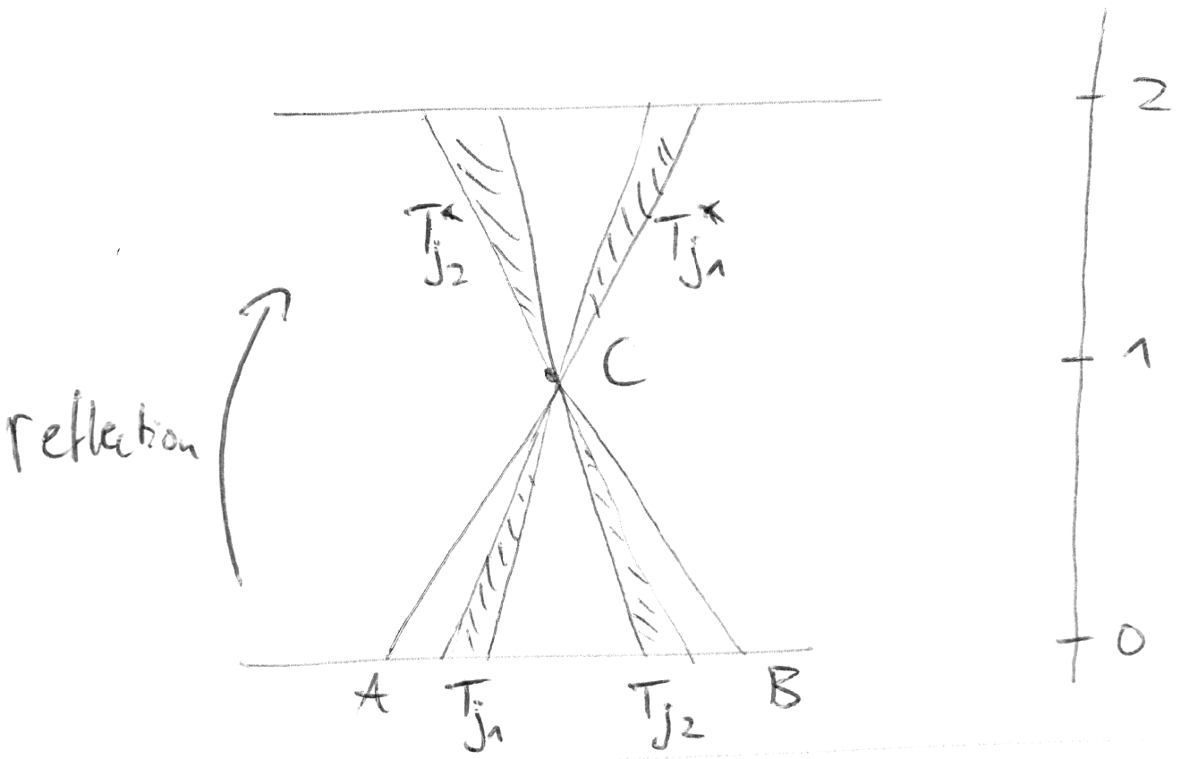
\includegraphics[height=5cm]{lec08_01}
		\caption{Obtaining mutually disjoint reaches by reflecting in $C$.}
	\end{figure}

	\begin{figure}[H]
		\centering
		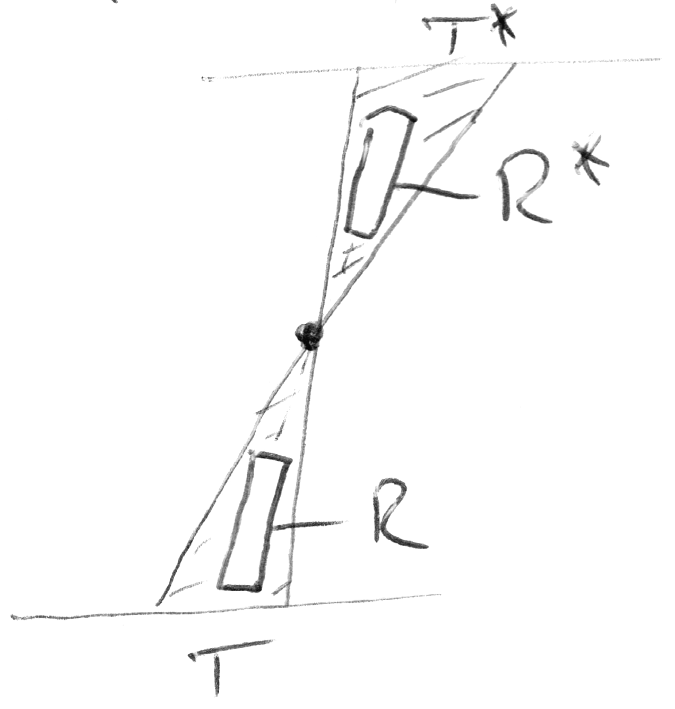
\includegraphics[height=5cm]{lec08_02}
		\caption{Go from triangles to rectangles by placing rectangles into the triangles with half the length.}
	\end{figure}

\end{proof}

\paragraph{Application} Maximal functions and counterexamples. Q: Given a collection $\C=\{C\}$ of sets, for which class of funcions do we have
\[\lim_{\diam(C)→0,\ c∈\C}\frac1{|C|}∫_Cf(x-y)\md y=f(x)\quad x-\text{a.e.}?\]
Seen:\[(M_\C f)(x)=\sup_{c∈\C}\frac1{|C|}∫_C|f(x)-y)|\md y\]
$\C=\{\text{bals}\}$, weak-type (1,1)inequality for $M_\C⇒$ a.e.\ convergenc of averages. A converse also holds!

$\{\mdμ_j\}_{j=1}^∞$ collection of finite, nonnegative measures on $ℝ^d:\supp(μ_j)⊂K⊂⊂ℝ^d$. Define the maximal operator \[(Mf)(x)=\sup_j|f*μ_j|(x).\]

\begin{pro}$1\leq p<∞$. Assume for each $f∈L^p(ℝ^d)$ that $(Mf)(x)<∞$ for some set of $x$ having positive measure. Then $f↦Mf$ if of wak-type $(p,p)$
	\[∃A<∞:|\{x∈ℝ^d:(Mf)(x)>α\}|\leq\frac A{α^p}\|f\|_{L^p} \quad(∀α>0)\]
\end{pro}

\begin{lem}
	$\{E_j\}$ collection of subsets of a fixed compact set: \[\sum_{j=1}^∞|E_j|=∞.\] Then there exists a sequenc of translates $F_j=E_jx_j$:
	\[\limsup F_j=\bigcap_{k=1}^∞(\bigcup_{j=k}^∞F_j)=ℝ^n\quad\text{(a.e.)}\]
\end{lem}
The above set equals $\{x∈ℝ^d:x∈F_j\text{ infinitely often}\}$.
\[\liminf F_j=\bigcup_{k=1}^∞(\bigcup_{j=k}^∞F_j)\]
is a subset.
\begin{proof}[Proof of Lemma]
	$Q⊂ℝ^d$ unit cube. $A_1,A_2⊂Q$. Then $∃h∈ℝ^d:|A_1∩(A_2-h)|\geq2^{-d}|A_1||A_2|$.
	\begin{figure}[h]
		\centering
		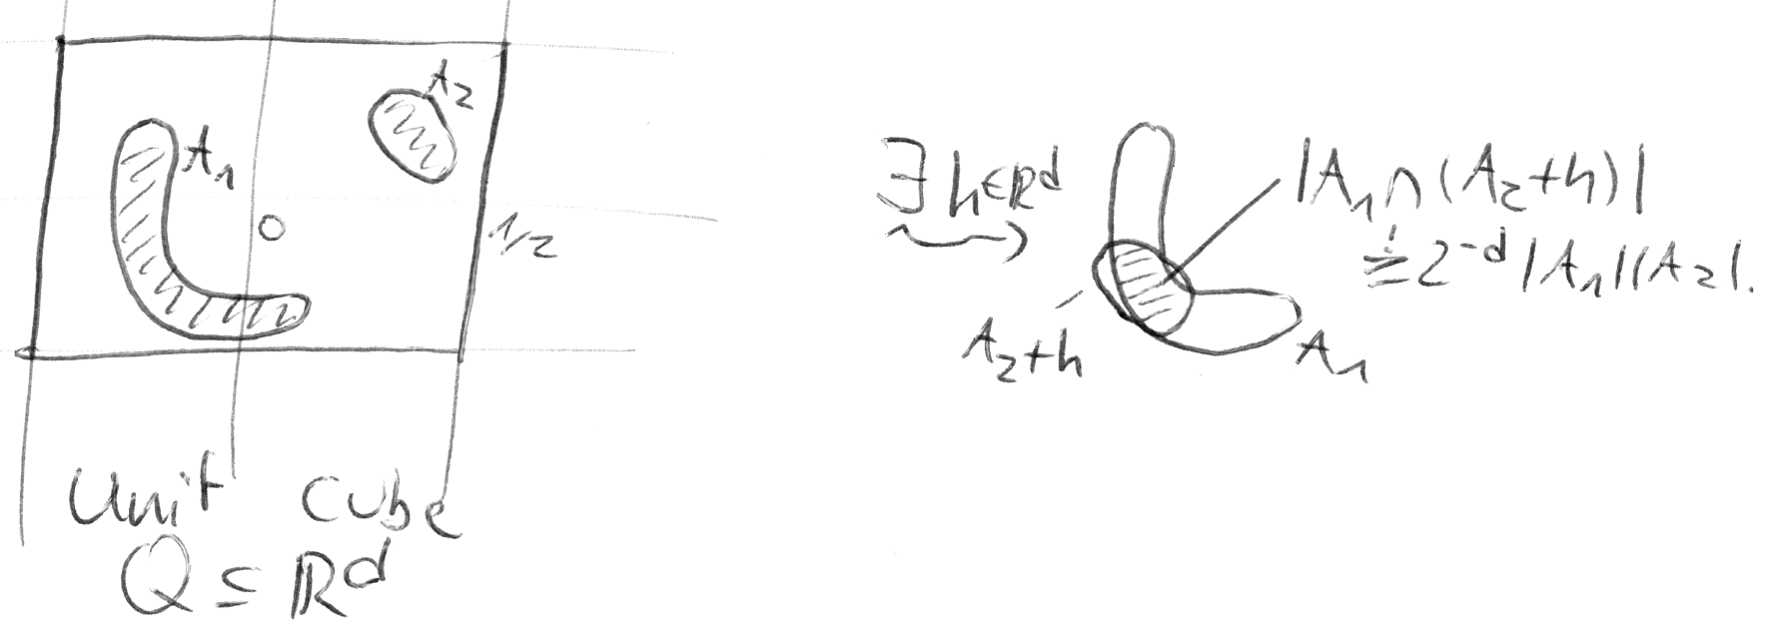
\includegraphics[height=5cm]{lec09_01}
		\caption{Translation of subsets $A_1$ and $A_2$ of a unit cube $Q$.}
	\end{figure}
	Why?
	\[η(x)=ι_{ℝ^d}χ_{A_1}(y)χ_{A_2}(x+y)\md y\simχ_{A_1}*χ_{A_1}(x)\]
	\[∫_{ℝ^d}|A_1||A_1|\]
	\[\supp(η)⊂Q^*\]
	$|Q^*|=2^d$. 
	\[∃h∈Q^*:η(h)\geq\avg_{Q^*}(η)=\frac1{|Q^*|}∫_{ℝ^d}η=\frac{|A_1||A_2|}{2^d}\]
	Wlog $\supp(E_j)⊂Q$.

	Step 2: There exist translates $F_j=E_j+x_j$ that cover $Q$ at least once.
	\[Q⊂\bigcup_j F_j\]
	Why? $F_1=E_1$. Suppose (inductively) that $F_1,…,F_{j-1}$ have been constructed. Let $A_1=Q∩(F_1∪…∪F_{j-1})^\complement$ and $A_2=E_j$. Step 1 $⇒∃h:|A_1∩(A_2-h)|\geq 2^{-d}|A_1||A_2|$. Set $F_j=A_2-h=E_j-h$. Let $p_j=|Q∩(F_1∪…∪F_j)|$. Then \[jvp_j=p_{j-1}+|\underbrace{Q∩(F_1∪…∪F_{j-1})^\complement}_{A_1}∩\underbrace{F_j}_{A_2-h}|=p_{j-1}+|A_1∩(A_2-h)|\geq p_{j-1}+2^{-d}|A_1||E_j|=p_{j-1}+2^{-d}(1-p_{j-1})|E_j|\]
	\[\therefore p_j-p_{j-1}\geq2^{-d}(1-p_{j-1})|E_j|\]
	\[\sum_{j=2}^∞(p_j-p_{j-1})=\lim_{j→∞}p_j-p_1\therefore\lim_jp_j=1\]
	Step 3: Decompose (twice) $\{E_j\}$ into a countable infinite number of subcollections so that on each subcollection the sum of the measures diverges.
\end{proof}
\begin{proof}[Proof of Proposition]
	Take a baoo $B$ sucth that $B\supset Q+K$. $\supp(F)⊂Q⇒\supp(F*⇔_j)⊂⇒\supp(Mf)⊂B$. Key: Estimate (*) (the violation of the weak type estimate) holds if $\supp(f)⊂Q$. For each $k,∃α_k>0∃g_k⊂L^p:\supp(g_k)⊂Q$ such that \[|\{x∈B:Mg_k(x)>α_\}|\geq\frac{2^k}{α_k^p}\|g_k\|_{L^p}^p\]
	Replace $g_k$ by $\tilde g_k=\frac k{α_k}g_k$.
	\[\frac{2^k}{k^p}\leq\frac{|\{x∈B:M\tilde g_k(x)>k\}|}{\|\tilde g_k\|_{L^p}^p}→∞\quad\text{as} k→∞\]
	$\therefore$ Tthere exists a sequence $\{f_k\}⊂L^p$ and a sequence of constans $R_k→∞$ such that (if $E_k=\{x∈B:M f_k(x)>R_k\}$)
	\[\sum_k|E_k|=∞\qquad\sum_k\|f_k\|_{L^p}^p<∞.\]
	\begin{rem} 
		$\mdμ_j\geq 0$ wlog $f_k\geq 0$. 
	\end{rem}
	By the lemma $∃\{x_k\}$ such that $F_k=E_k+x_k$ satisfy $\limsup F_k=ℝ^d$ (a.e). Let
	\[\tilde f_k(x)=f_k(x+x_k),\qquad F(x)=\sup_k\tilde f_k(x)\]
	Then \[M(F)=\sup_j|F*⇔_j|=\sup_j|(\sup_k\tilde f_k)*⇔_j|\geq\sup_k\sup_j|\tilde f_k*μ_j|=\sup_kM(\tilde f_k)\]
	Also $M(\tilde f_k)>R_k$ on $F_k\therefore M(F)=∞$ a.e. Check $f∈L^p$: \[|F|^p=|\sup_k\tilde f_k|^p\leq\sum_p|\tilde f_k|^p\]
	\[\|F\|_{L^p}^p\leq\sum_k\|f_ku|_{L^p}^p<∞\]
	Full conclusion
	\[f=\sum fχ_{Q_j}=:\sum f_j\]
	\[M(f)\leq\sum_jM(f_j)\]
\end{proof}

\begin{exa}%1
	Rectangles with arbitrary orientation
	\[\C=\R=\{\text{\highl{all} retangles in $ℝ^2$ centered at $0$}\}\]
	\begin{figure}[H]
		\centering
		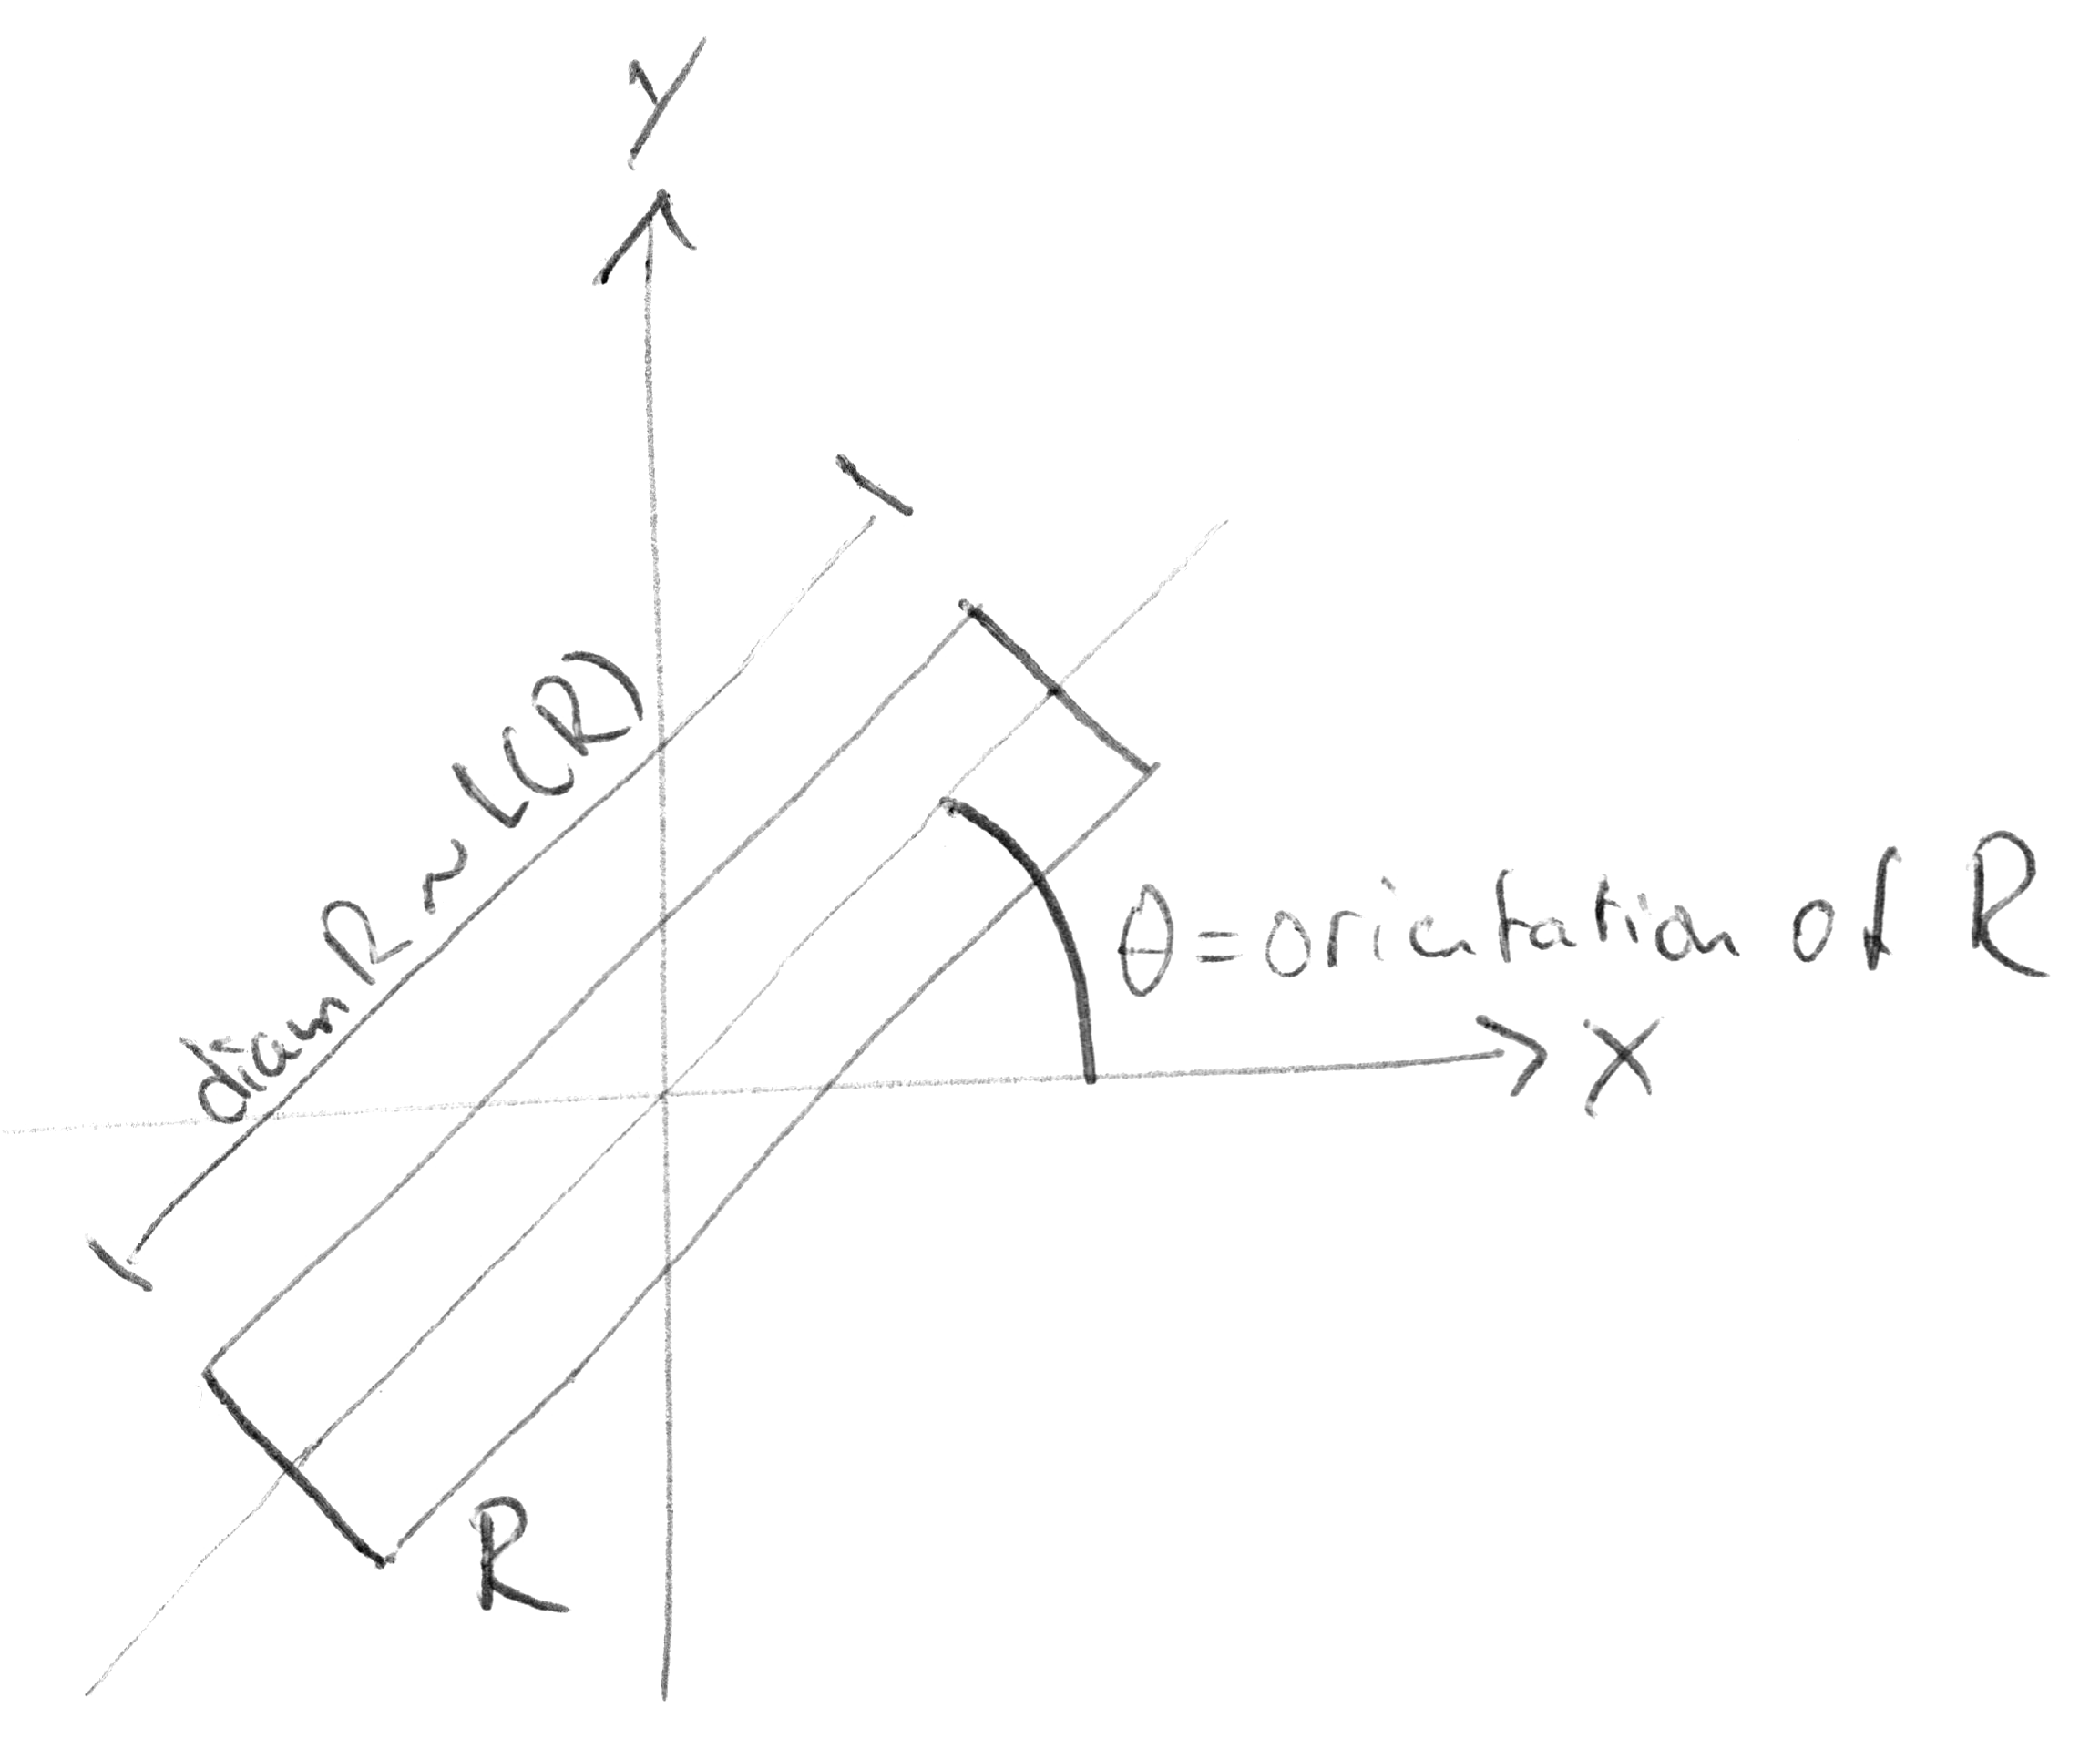
\includegraphics[height=7cm]{lec09_02}
	\end{figure}
\end{exa}
\begin{cor}
	Given $1\leq p<∞,∃f∈L^p(ℝ^)$ such that \[\limsup_{\diam(R)→0R∈\R}\frac1{|R|}∫_Rf(x-y)\md y=∞\quad (x-\text{a.e.})\]
\end{cor}
Idea: Use the $ε$-Kakeya set to show that $M$ is not weak $(p,p)$
\[(Mf)(x)=\sup_{\diam(R)<8}\frac1{|R|}|∫_Rf(x-y)\md y|\]
Let $E=\bigcup_{j=1}^{2^N}R_j$ as before. $\|χ_E\|_{L^p}^p=|E|<ε$. If $x∈\tilde R_j$, then $∃$ rectangle $R$ such that
\begin{itemize}
	\item $R$ is centered at $x$
	\item $\diam(R)\leq 8$
	\item $|R∩R_j|\geq\frac1{12}|R|$
\end{itemize}
\begin{figure}[H]
	\centering
	\subfigure{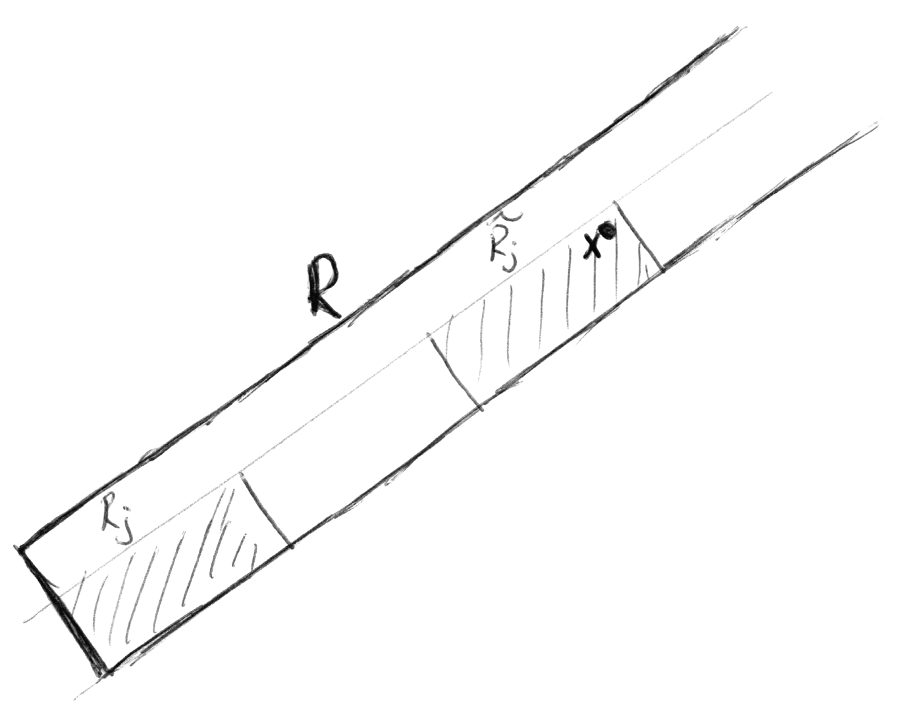
\includegraphics[height=4cm]{lec09_03}}\\
	\subfigure{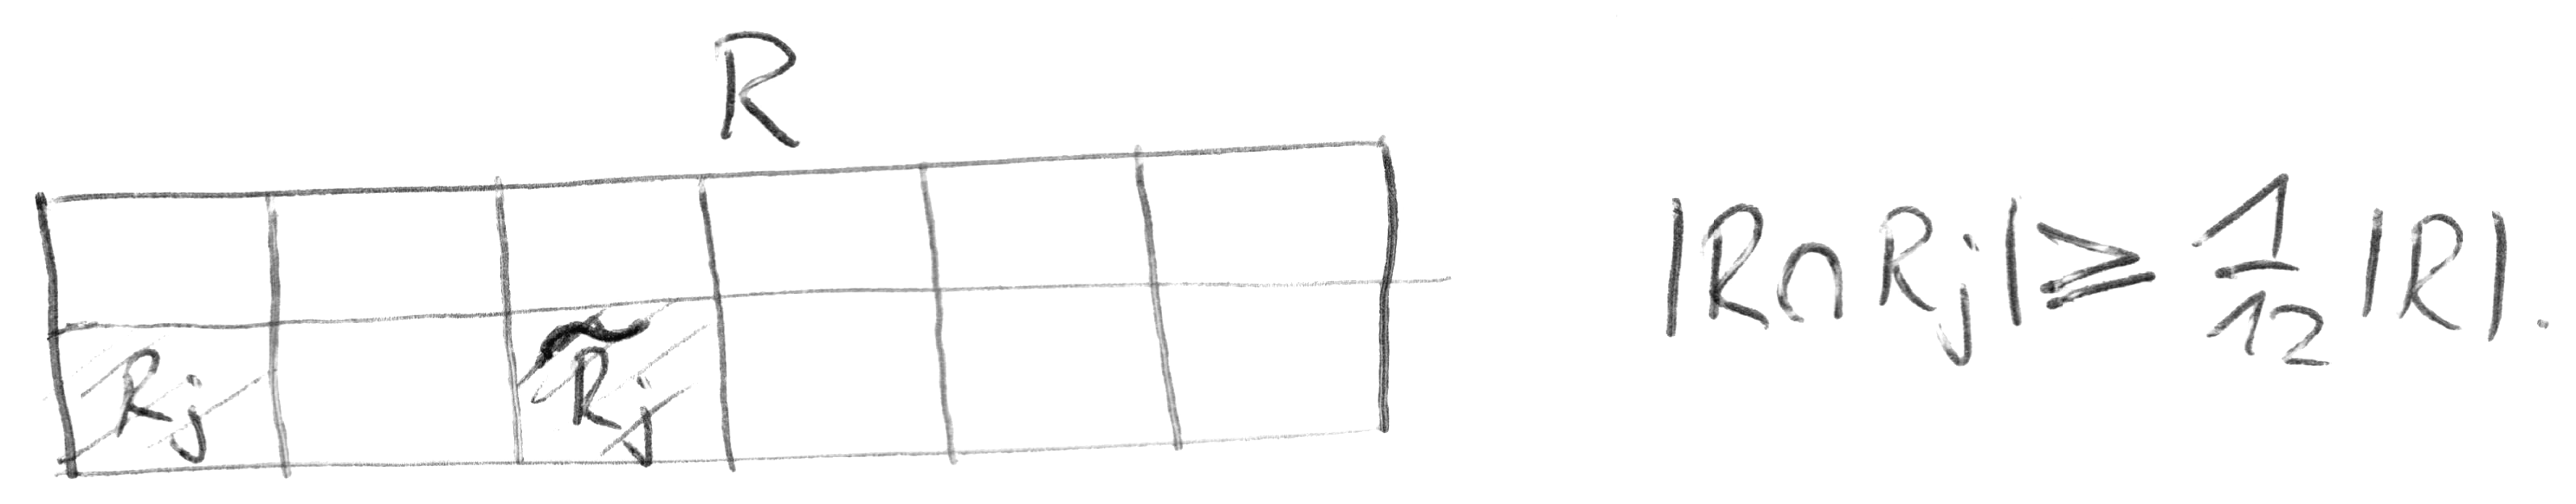
\includegraphics[height=1.5cm]{lec09_04}}
\end{figure}
$y∈x-E=-(E-x),\ y-x∈-E,\ x-y∈ E$
\[M(χ_E)(x)\geq\intbar_{R-x}χ_E(x-y)\md y=\frac{|(R-x)∩(E-x)}{|R|}\geq\frac1{12}\]

Conclusion: $Mχ_E\geq\frac1{12}$ on the set $\bigcup_{j-1}^{2^N}\tilde R_j$ (of measure 1)
\[∀A>0∃\text{set}E|\{x∈ℝ^d:Mχ_E>α\}|\leq Aα^{-p}\|χ_E\|_{L]p}^p\]
does not hold! $\therefore M$ is not of weak typ $(p,p)$.

Note, that this is not the complete proof. Therefore still have to replace 8 by $δ$.

\paragraph{Bochner-Ries summability}
Q: In which way does Fourier inversion hold? (In $L^p(ℝ^d)$)
\[f(x)=∫_{ℝ^d}\hat f(ξ)e^{2πixξ}\mdξ=\lim_{R→∞}\underbrace{∫_{|ξ|<R}\hat f(ξ)(1-\frac{|ξ|^2}{R^2})^δe^{2πixξ}\mdξ}_{f*k_δ}?\]
for suitable $δ\geq 0$.
\[δ>\frac{d-1}2⇒k_δ∈L^1(ℝ^d)\]
\[δ\leq \frac{d-1}2\]
\[δ=0\text{ today}\]
$d=1$: The second equality holds in $L^p$-norm ($1<p<∞$) $\impliedby L^p$ boundedness of Hilbert transform

It also holds a.e.\ $(p=2$ Carleson '66 $1<p<∞$ Hunt '68)

$d\geq 2$ Let us only consider norm convergence
\[f↦(S^δf)(x)=∫_{|ξ|\leq 1}\hat f(ξ)(1-|ξ|^2)^δe^{2πixξ}\md ξ\]
\[Sf(x)=∫_{|ξ|\leq 1}\hat f(ξ)e^{2πixξ}\mdξ\]
\[\widehat{Sf}=1_{|ξ|\leq 1}\hat f\]
($\widehat{Hf}=iπ\sgnξ\hat f$)
\[\|Sf\|_{L^2(ℝ^d)}=\|\widehat{Sf}\|_{L^2}=\|1_{|ξ|\leq 1}\hat f\|_{L^2}\leq\|\hat f\|_{L^2}=\|f\|_{L^2}\]
He said something about every bounded operator can be written like this or so? 
Fourier multiplier $S$ is bounded iff multiplier function is bounded.

\begin{theo}[C.Fefferman '71 -- Annals of mathematics "The multiplier problem for the ball"]
	Suppose $q\geq 2$ and $p\neq 2$. Then the operator $S$ (initially defined on $L^p∩L^2$) is not extendable to a bounded operator from $L^p(ℝ^d)$ to itself.
\end{theo}
(What is $q$?)

\begin{proof}
	Let $B⊂ℝ^d$ ball, let $S_B$ be the multiplier orator associated to $B$:
	\[\widehat{S_Bf}=1_B\hat f.\]
	Given $u∈S^{d-1}⊂ℝ^d$, let $S^n$ be the multiplier operator associated to the half-space with normal $u$:
	\[\widehat{S^uf}=1_{\{ξu>0\}}\hat f\qquad (S^uf)(x)=∫_{ξu>0}\hat f(ξ)e^{2πixξ}\mdξ\]
	Upshot: $L^p$-bound for $S$ implies an $L^p$ vector-valued inequality for $S_B$s and $S_u$s.

	\begin{lem}[Y. Méyer]
		Suppose \[\|Sf\|_{L^p}\leq A_p\|f\|_{L^p}\]
		$f∈(L^2∩L^p)(ℝ^d)$ holds for some $p∈[1,∞]$. Suppose $f_1,…,f_M∈L^2∩L^p,\ u_1,…,u_M∈S^{d-1}⊂ℝ^d$. Then
		\begin{equation}
			\|(\sum_{j=1}^M||S^{u_j}(f_j)|^2)^{\frac12}\|_{L^p(ℝ^d)}\leq A_p\|(\sum_{j=1}^M|f_j|^2)^{\frac12}\|_{L^p(ℝ^d)}
			\label{eq:meyer}
		\end{equation}
		where $A_p$ is the same constant as above.
	\end{lem}
	\begin{proof}[Proof of Lemma]
		Step 1: $B=B_R=$ ball of radius $R$ centered at $0$. Then
		\begin{equation}
			\|S_B(f)\|_{L^p}\leq A_p\|f\|_{L^p}\quad(g∈L^2∩L^p)
			\label{eq:sbnorm}
		\end{equation}
		Why? Scaling: \[δ_R(g)(x)=g(\frac xR)\] Check $δ_{R^{-1}}∘ S∘ δ_R=S_{B_R}$ since $S=S_{B_1}$. $\hat δ_ρ(g)(ξ)=R^d\hat g(Rξ)$.

		Step 2: $M$ balls. ($p<∞$) $f=(f_1,…,f_M)$ given $M$-tuple of functions. $T(f):=(Tf_1,…,Tf_M)$. Given a unit vector $ω=(ω_1,…,ω_M)∈ℂ^M$, let
		\[S_ω(f)=\sum_{j=1}^M\barω_jS_B(f_j)=S_B(\sum_j\barω_jf_j)=S_B(f_ω)\qquad f_ω=\sum_{j=1}^M\barω_jf_j\]
		\begin{equation}
			\eqref{eq:sbnorm}⇒∫_{ℝ^d}|S_ωf(x)|^p\md x\leq A_p^k∫_{ℝ^d}|f_ω(x)|^p\md x
			\label{eq:swnorm}
		\end{equation}
		$(S_ωf)(x)=?$. $x,y∈ℂ^M,\ \langle x,y\rangle=\sum_{i=1}^Mx_j\bar y_j$
		\begin{align*}
			S_ω(f)(x)&=S_B(f_ω)(x)=S_B(\sum_{j=1}^M\barω_jf_j)(x)=\sum_{j=1}^M\barω_jS_B(f_j)(x)|=|\langle S_B(f)(x),ω\rangle|\\
			   &=|S_B(f)(x)||\langle\frac{S_B(f)(x)}{|S_B(f)(x)|},ω,\rangle|=(\sum_{j=1}^M|S_B(f_j)(x)|^2)^{\frac12}|φ(ω,S_B(f)(x))|
		\end{align*}
		Integrate both sides of \eqref{eq:swnorm} with respect to $ω$ (before integrating in $x$).
		\begin{align*}
			\text{LHS}&=∫_{ℝ^d}(∫_{|ω|=1}|S_ω(f)(x)|^p\mdω)\md x\\
			   &=∫_{ℝ^d}(\sum_{j=1}^M|S_B(f_j)(x)|^2)^{\frac p2}\ub{(∫_{|ω|=1}|Φ(ω,S_B(f)(x)|^p\mdω)\md x)}_{γ_p})\md x
		\end{align*}
		\[0\neq γ_p=∫_{|ω|=1}|Φ(ω,1)|^p\mdω\]
		For fixed $ν∈S^{d-1}$ $∫_{S^{d-1}}|\langleω,ν\rangle|^p\mdσ_ω=ω_{d-2}∫_{-1}^1(1-t^2)^{\frac{d-3}2}\md t$.

		Similarly,
		\[\text{RHS}=∫_{ℝ^d}(\sum_{j=1}^M|f_j(x)^2)^{\frac p2}\md xγ_p\]
		\[\eqref{eq:swnorm}⇒\|(\sum_{j=1}^M|S_B(f_j)|^2)^{\frac12}\|_{L^p(ℝ^d)}\leq A_p\|(\sum_{j=1}^M|f_j|^2)^{\frac12}\|_{L^p(ℝ^d)}\]

		Step 3: From balls to half-spaces

		$B_R^u=$ ball of radius $R$ centered at $Ru$. Upshot: $B_R^u→\{ξu>0\}$ as $R→∞$. 

		Translation
		\[(T_yf)(x)=f(x-y)\]
		\[\widehat{T_yf}(ξ)=e^{iξy}\hat f(ξ)\]
		\[S_{B_R^u}(f)(x)=e^{2πiuRx}S_{B_R}(fe^{-2πiuRx})\]
		\eqref{eq:meyer} implies
		\[\|(\sum|S_{B_R^{u_j}}(f_j)|^2)^{\frac12}\|_{L^p}\leq A_p\|(\sum|f_j|^2)^{\frac 12}\|_{L^p}\]
		Let $R→∞$ to finish:
		\[\therefore S_{B_R^{u_j}}(f_j)→S^{u_j}(f_j)\quad R→∞(\text{ in }L^2)\]
		$\therefore$ there exists an almost everywhere converging subsequence, done.
	\end{proof}

	$\widehat{Sf}=1_{B(0,1)}\hat f$. $S$ is not bounded in $L^p(ℝ^d)$ unless $d=1$ or $p=2$. Focus on multiplier operator for the half-space ($S^u$), $d=1$.
	\[(S^+f)(x)=∫_0^∞\hat f(ξ)e^{2πixξ}\mdξ\quad(f∈L^2)\]
	\begin{equation}
		|(S^+f)(x)|\geq\frac c{|x|}\quad\text{if }|x|\geq\frac12
		\label{eq:spgeqcdx}
	\end{equation}
	\begin{proof}
		\[(S^+f)(x)=\lim_{ε→0}∫_0^∞\hat f(ξ)e^{2πi(x+iε)ξ}\mdξ\quad\text{in }L^2\]
		\[∫_{-∞}^∞(∫_0^∞e^{-2πiyξ}e^{2πi(x+iε)ξ}\mdξ)f(y)\md y=\frac1{2πi}∫_{-\frac12}^{\frac12}\frac1{y-x-iε}\md y\]
		This has absolute value $\lesssim c{|x|}$ if $|x|\geq\frac12$.

		Alternative proof: $|H(f)(x)|\geq|x|^{-1}$ for large $x$, $S^+=\frac12(I+iH)$.
		\begin{figure}[H]
			\centering
			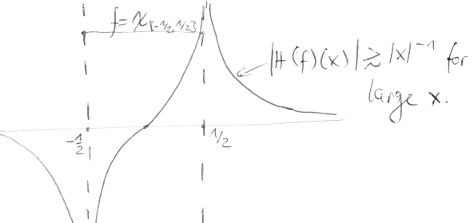
\includegraphics{lec10_01}
		\end{figure}
	\end{proof}
	\begin{figure}[H]
		\centering
		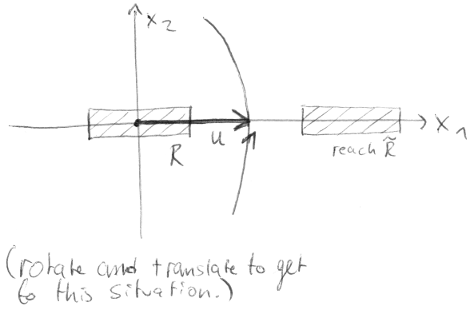
\includegraphics{lec10_02}
	\end{figure}
	For $R=(-\frac12,\frac12)\times(-\frac1{2^{N+1}},\frac1{2^{N+1}})$
	\[1_R=1_{(-\frac12,\frac12)}\otimes1_{(-2^{-(N+1)},2^{-(N+1)})}\]
	If $u$ points in the direction of $x_1$ then
	\[(S^u1_R)(x_1,x_2)=(S^+1_{(-\frac12,\frac12)})(x_1)1_{(-2^{-(N+1)},2^{-(N+1)})}(x_2)\]
	\[\eqref{eq:spgeqcdx}⇒|S^u(1_R)|\geq c'1_{\tilde R}\]
	Similarly for any $1\times 2^{-N}$ rectangle $R_j$. $u_j∈S^1$ in the positive direction of the longest side of $R_j$. Rotate and translate, then we get
	\begin{equation}
		|S^{u_j}(1_{R_j})|\geq c'1_{\tilde R_j}
		\label{eq:suj1rgeq}
	\end{equation}
	Take $R_1,…,R_{2^N}$ to be the collection given by $ε$-Kakeya construction, plug that into result from lemma, get a contradiction.

	Key: $p<2$ and $d=2$.

	Lemma with $f_j=1_{R_j}$ and $M=2^N$
	\begin{align*}
		c'&\leq\|(\sum_{j=1}^{2^N}|S^{u_j}(1_{R_j})|^2)^{\frac12}\|_{L^p(ℝ^2)}\qquad\eqref{eq:suj1rgeq},\ |\bigcup\tilde R_j|=1\\
		  &\leq A_p\|(\sum_{j=1}^{2^N}|1_{R_j}|^2)^{\frac12}\|_{L^p(ℝ^2)}=A_p(\ub{∫_E(\sum_{j=1}^{2^N}|1_{R_j}|^2)^{\frac p2}\md x}_I)^{\frac1p}
	\end{align*}
	\begin{align*}
		I&\leq|E|^{\frac1q}(∫(\sum|1_{R_j}|^2)^{\frac p2\frac2p}\md x)^{\frac1p\frac p2}\qquad\tx{Hölder}\\
   &=|E|^{\frac1q}\sum_{j=1}^{2^N}|R_j|=|E|^{\frac1q}
	\end{align*}
	\[E=\bigcup_{j=1}^{2^N}R_j,\quad |E|<ε,\quad \frac1q+\frac1{p/2}=1,\quad \frac1q=1-\frac p2,\quad\frac1{pq}=\frac1p(1-\frac p2)>0\]
	In the end we get
	\[c'\leq A_pε^{\frac1{pq}}.\]
	Let $ε→0^+$ to finish.

	$d>2$:
	\[f_j(\ub x_{∈ℝ^d})=f_j(x_1,x_2,\ub{x'}_{∈ℝ^{d-2}})=1_{R_j}(x_1,x_2)f(x')\quad f∈S(ℝ^{d-2})\]
	$p>2$:
	\[\langle Sf,g\rangle=\langle\widehat{Sf},\hat g\rangle=\langle 1_B\hat f,\hat g\rangle=\langle \hat f,1_B\hat g\rangle=\langle f,Sg\rangle\quad S=S^*\]
\end{proof}

\paragraph{Oscillatory integrals in harmonic analysis}
Stein (VIII,IX), Stein-Shakarchi (Chapter 8), Sogge
\begin{itemize}
	\item averaging operators
	\item restriction theory
	\item Bochner-Riesz summability
\end{itemize}
\subparagraph{Motivation (in $ℝ^3$)}
\[(Af)(x)=\dashint_{S^2}f(x-y)\mdσ_y=\f1{4π*σ}(x)\]
$σ$ surface measure in $S^2$.

Smoothing properties:
\begin{equation}
	\|\f∂{∂x_j}A(f)\|_{L^2(ℝ^3)}\lesssim\|f\|_{L^2(ℝ^3)}\quad(j=1,2,3)
	\label{eq:smoothprop}
\end{equation}
$f∈L^2⇒$
\[\|f*σ\|_{L^2}\leq\|f\|_{L^2}\ub{|σ|(ℝ^3)}_{<∞}\] (use Minkowski integral inequality) $\therefore f*σ∈L^2$ if $f∈L^2$.

Idea $\widehat{(f*σ)}=\hat f\hatσ$
\[\widehat{(\f∂{∂x_j}A(f))}(ξ)=ξ_j\hat f(ξ)\hatσ(ξ),\]
so we should study $\hatσ$.

without loss of generality $ξ=(0,0,|ξ|)$ because the integral is spherically symmetric.
\[\hatσ(ξ)=∫_{S^2}e^{-2πiωξ}\mdσ_ω=2π∫_0^πe^{-2πi|ξ|\cosθ}\sinθ\md=2π∫_{-1}^1e^{2πi|ξ|t}\md t=\f{2\sin(2π|ξ|)}{|ξ|}\]
\[t=\cosθ\quad\md t=\sinθ\mdθ\]
\[\therefore|\hatσ(ξ)|\lesssim(1+|ξ|)^{-1}\]
\eqref{eq:smoothprop} follows from this and Plancherel.

This also generalizes to higher dimensions. There we get a factor $(1-t^2)^{\f{d-3}2}$ in the last integral.

\paragraph{Oscillatory integrals}
\[I(λ)=∫_{ℝ^d}e^{iλϕ(x)}ψ(x)\md x\]
where $λ∈ℝ$ is the oscillatory parameter, $ϕ∈C^∞(ℝ^d,ℝ)$ the phase and $ψ(x)∈ℂ$ the amplitude.

Q.: How does $I(λ)$ behave for large $|λ|$? General principle: Main contribution comes from the critical points of the phase, $x_0:\ ∇ϕ(x_0)=0$.

\paragraph{Principle of non-stationary phase}
$ϕ∈C^∞,\ ψ∈C^∞_0:|∇ϕ(x)|> 0\ (∀x∈\suppψ)$. Then for any $N∈ℕ$
\[|I(λ)|\leq c_N|λ|^{-N}\]
\begin{proof} Integration by parts (in a more complicated version)
\end{proof}
$d=1$:
\[I_1(λ)=∫_a^be^{iλϕ(x)}\md x\]
\[0<a<b<∞\quadψ(x)=χ_{[a,b]}(x)\quad\tx{which is rough!}\]
This means we will not get such a fast decay
\begin{lem}[van der Corput (I)]
	$ϕ∈C^2,\ ϕ'$ monotonic, $|ϕ'(x)|\geq 1\ (∀x∈[a,b])$. Then
	\[|I_1(λ)|\leq\f3{|λ|}\quad(∀λ>0)\]
\end{lem}
\begin{rem}
	\begin{enumerate}
		\item $3$ is neither important nor sharp; independence of $a,b,ϕ$ is the key!
		\item Order of decrease in $λ$ is sharp ($ϕ()=x\therefore I_1(λ)=\f{e^{iλb}-e^{iλa}}{iλ}$)
		\item monotonicity of $ϕ'$ is essential
	\end{enumerate}
\end{rem}
\begin{proof} Integrate by parts(…)
\end{proof}
What if critical points are present? ($d=1$)

$x_0:ϕ'(x_0)=0$ (critical point) and $ϕ''(x_0)\neq 0$ (non degenerate), e.g.\ $ϕ(x)=x^2,\ x_0=0$. In this case
\[∫_ℝe^{iλx^2}ψ(x)\md x=c_0λ^{\f{-1}2}+\ord(|λ|^{-\f32})=\sum_{k=0}^Na_xλ^{-\f12-k}+\ord(|λ|^{-\f32-N})\quad(∀N,\ λ→∞)\]
\begin{lem}[van der Corput (II)]
	$ϕ∈C^2[a,b],\ |ϕ''(x)|\geq 1\ (∀x∈[a,b])$. Then
	\[|I_1(λ)|\leq\f8{λ^{\f12}}\quad(∀λ>0)\]
\end{lem}
\begin{rem} More generally: $\ord(|λ|^{\f1k})$ if $|ϕ^{(k)}|\geq 1$.
\end{rem}
\begin{proof} Integration by parts not needed. Instead split up region in small area around critical point with properly chosen size, and rest, and then use results from above.
	%figure here?
\end{proof}
\begin{cor} Same assumptions as van der Corput (II). $ψ∈C^1[a,b]$.
	\[|∫e^{iλϕ(x)}ψ(x)\md x|\leq c_ψλ^{\f{-1}2}\]
\end{cor}
Application: Asymptotics of Bessel functions
\[J_m(r)=\f1{2π}∫_0^{2π}e^{ir\sin x}e^{-imx}\md x\quadϕ(x)=\sin x,\quad ψ(x)=e^{-imx}\quad(m∈ℤ)\]

\begin{cor}
	\[|J_m(r)|\leq cr^{-\f12}\quad r→∞\]
\end{cor}
Recall: Averaging operator in $ℝ^d\ (d>1)$ is 
\[(Af)(x)=(f*σ)(x)\quadσ\tx{ surface measure on $S^{d-1}$}\]
\begin{theo}
	$f⇒A(f)$ is bounded from $L^2(ℝ^d)$ to $L^2_k(ℝ^d)$ with $=\f{d-1}2$.
\end{theo}
\begin{proof}
	\[\hatσ(ξ)=2π|ξ|^{-\f d2+1}\ub{J_{\f d2-1}(2π|ξ|)}_{=\ord(|ξ|^{-\f12}),\ |ξ|→∞}\]
	\[\therefore|\hatσ(ξ)|=\ord(|ξ|^{-\f{d-1}2})\quad|ξ|→∞\]
\end{proof}	

"What is van der Corput's lemma in higher dimension?" (Carbery-Wright, 2000)

\[I(λ)=∫_{ℝ^d}e^{iλϕ(x)}ψ(x)\md x\]
($ϕ$ smooth, $ψ$ smooth, compactly supported)

nondegeneracy hypothesis
\[\det(∇^2ϕ)(x)\neq 0\quad∀x∈\supp(ψ)\]

\begin{theo} Under above assumptions
	\[|I(λ)|=\ord(|λ|^{-\f12})\quadλ→∞\]
\end{theo}	
\begin{rem}
	\begin{enumerate}
		\item Decay rate is sharp
		\item Proof uses $TT^*$ method: $|I(λ)|^2=I(λ)\overline{I(λ)}$
		\item variant: $\rk(∇^2ϕ)\geq m$ for some $0<m\leq d$ on $\supp(ψ)$. Then
			\[|I(λ)|=\ord(|λ|^{-\f m2})\]
	\end{enumerate}
\end{rem}
\paragraph{Application:} Fourier transform of surface-carried measures

Recall: $(S^{d-1},σ)$
\[|\hatσ(ξ)|\lessim(1+|ξ|)^{-f{d-1}2}\]
(not a Bessel coincidence)

(local) $C^∞$-hypersurface $M$. After translation and rotation $x_0=0$, $T_{x_0}M=\{x_d=0\}$. $M$ can be represented as
\[M=\{(x',x_d)∈B⊂ℝ^d:x_d=φ(x')\}\]
Can arrange $φ(0)=0=(∇_{x'}φ)(x')|_{x'=0}$.
\[φ(x')=\f12\sum_{k,j=1}^{d-1}\ub{\f{∂^2φ}{∂x_k∂x_j}}_{(a_{jk})}x_kx_j+\ord(|x'|^3)=\f12\sum_{j=0}^{d-1}kjx_j^2+\ord(|x'|^3)\]
$(a_{jk})$ $(d-1)\times(d-1)$ $ℝ$-valued symmetric matrix $\therefore$ diagonizable. $k_j$ principal curvaturos of $M$ at $x_0$. $k:=\prod_{j=1}^{d-1}k_j$ is the Gaussian curvature of $M$ at $x_0$ ($k=\det(∇^2φ)$)

E.g.\ 
\begin{enumerate}
	\item $S^{d-1}⊂ℝ^d$. $k_j=1\ (∀j)\therefore k=1$
	\item $\{x_3=\ub{x_1^2-x_2^2}_{φ(x_1,x_2)}\}⊂ℝ^3$, $\f12∇^2φ(x)=
	\begin{pmatrix}1&0\\0&-1\end{pmatrix}$
	\item $\{x_1^2=|x'|^2:x\neq 0\},\ x'∈ℝ^{d-1}$. $d-2$ identical nonvanishing principal curvatures $x_d^{-2}$ +1 vanishing principal curvature.
\end{enumerate}
\paragraph{surface measure $σ$}
\[∫_Mf\mdσ=∫_{ℝ^{d-1}}f(x',φ(x'))\ub{\sqrt{1+|∇_{x'}φ(x')|^2}\md x'}_{\mdσ\tx{ in our coordinate sys.}}\]
\[\mdμ=ψ\mdσ,\quadψ∈C^∞_0(M,σ)\]
is a surface carried measure.
\[\hatμ(ξ)=∫_Me^{-2πixξ}\mdμ(x)=∫_Me^{-2πixξ}ψ(x)\mdσ_x\]
is bounded on $ℝ^d$ because $|μ|(ℝ^d)<∞$.
\begin{theo} Hypersurface $M⊂ℝ^d$ with nonvanishing Gaussion curvature at each point of $\supp(ψ)$. Then
	\[|\hatμ(ξ)|=\ord(|ξ|^{-\f{d-1}2}),\quad|ξ|→∞\]
\end{theo}
\begin{cor} If $M$ has at last $m$ non vanishing principal curvatures (at each point of $\supp(ψ)$), then
	\[|\hatμ(ξ))|=\ord(|ξ|^{-\f m2}),\quad |ξ|→∞\]
\end{cor}

Last time: oscillatory integrals and averaging operators
\[(Af)(x)=(F*σ)(x)=\dashint_{\se^{d-1}}f(x-y)\mdσ_y\quad(d>1)\]
Smoothin property: $f\mapsto A(f)$ is bounded from $L^2(ℝ^d)$ to $L^2_k(ℝ^d)$ with $k=\f{d-1}2$. Here we used
\[|\hatσ(ξ)|\lesssim|ξ|^{-\f{d-1}2}.\]

A few weeks ago:
\[R(f)(t.γ)=∫_{P_{t,γ}}f\]
where $P_{t,γ}=\{x∈ℝ^d:xγ=t\}$.
\[R^*(f)(γ)=\sup_{t∈ℝ}|R(f)(t,γ)|\]
if $d\geq 3$ then
\[∫_{\se^{d-1}}R^*(f)(γ)\mdσ_γ\lesssim\|f\|_{L^2}+\|f\|_{L^2}\]
This estimate was based on
\[∫_{\se^{d-1}}∫_{-∞}^∞|\hat R(f)(λ,γ)|^2|λ|^{d-1}\mdλ\mdσ_γ=2∫_{ℝ^d}|f(x)|^2\md x\]
due to $\hat R(f)(λ,γ)=\hat f(λγ)$. Consider $d=3$ then this becomes
\begin{equation}
	∫_{\se^2}∫_ℝ|\f\md{\md t}R(f)(t,γ)|^2\md t\mdσ_γ=8π^2∫_{ℝ^3}|f(x)|^2\md x
	\label{eq:dradonr3bound}
\end{equation}
by Plancherel $t\leftrightarrowλ$. Note, that something like this also holds for higher dimensions.

Now consider the following "linearized" version of the Radon transform:
\[R_B(f)=∫_{ℝ^{d-1}}f(y',x_d-B(x',y'))\md y'=∫_{M_x}f\]
where $x=(x',x_d)∈ℝ^{d-1}\timesℝ,\ y=(y',y_d)$ and $B:ℝ^{d-1}\timesℝ^{d-1}→ℝ$ is a nondegenerate bilinear form, and 
\[M_x=\{(y',y_d)\ |\ y_d=x_d-B(x',y')\}.\]
E.g.\ $B(x',y')=\langle x',y'\rangle$ (usual inner product on $ℝ^d$). $y_d=x_d-\langle x',y'\rangle\iff\langle x',y'\rangle+y_d=x_d\iff\langle (x',1),(y',y_d)\rangle=x_d$. The map
\begin{align*}
	ℝ^d&→\{\tx{affine hyperplanes on $ℝ^d$}\}\\
	x&↦M_x
\end{align*}
is injective and surjective onto $\{\tx{hyperplanes not orthogonal to $M_0=\{x_d=0\}$}\}$. The excerpted collection of hyperplanes is lower dimensional, so we can think of $R_B$ as a substitute for $R$.

An analogue of \eqref{eq:dradonr3bound} is
\[∫_{ℝ^d}|\f∂{∂x_3}R_B(f)(x)|^2\md x=c_B∫_{ℝ^3}|f(x)|^2\md x\]
for $f∈C^0_0(ℝ)$
\begin{proof}

	\begin{align*}
		∫_{ℝ^3}|\f∂{∂x_3}R_B(f)(x)|^2\md x&=∫_ℝ∫_{ℝ^2}|\ub{(\f∂{∂x_3}R_B(f))^∧(x',ξ_3)}_{=2πξ_3∫_{ℝ^2}e^{-2πiξ_3B(x',y')}\hat f(y',ξ_3)\md y'}|^2\md x'\mdξ_3&x=(x',x_3)
	\end{align*}
	The last equality follows from
\begin{align*}
\hat R_B(f)(x',ξ_3)&=∫_ℝe^{-2πiξ_3x_3}R_B(f)(x',x_3)\md x_3\\
		    &=∫e^{-2πiξ_3x_3}∫_{ℝ^2}f(y',\ub{x_3-B(x',y')}_{y_3})\md y'\md x_3\\
				  &=∫∫_{ℝ^{2+1}}e^{-2πiξ_3(y_3+B(x',y'))}f(y'y_3)\md y'\md y_3\\
							      &=∫_{ℝ^2}e^{-2πiξ_3B(x',y')}\ub{(∫_ℝe^{-2πiξ_3y_3}f(y',y_3)\md y_3)}_{\hat f(y',ξ_3)}\md y'
\end{align*}
	Since $B$ is nondegenetare $∃C:ℝ^2→ℝ^2$ linear, invertible such that $B(x',y')=\langle C(x'),y'\rangle$. Changle variables $ξ_3C(x')=u∈ℝ^2$ is well defined since $C$ is invertible. $\thereforeξ_3B(x',y')=\langleξ_3C(x'),y'\rangle=\langle u,y'\rangle\thereforeξ_3^2|\det C|\md x'=\md u$. Then the first integral becomes
	\[∫_ℝ∫_{ℝ^2}|∫_{ℝ^2}e^{-2πiuy'}\hat f(y',ξ_3)\md y'|^2\f{\md u}{|\det C|}\md ξ_3\simeq∫∫|\hat f(y',ξ_3)|^2\md y'\md ξ_3\simeq∫_{ℝ^3}|f(y)|^2\md y\]
	by 2D-Plancherel $y'\leftrightarrow u$ and 1D-Plancherel $ξ_3\leftrightarrow y_3$.
\end{proof}
\paragraph{Rotational curvature}
Both the averaging operator $A$ and the Radon transform $R_B$ are of the form $f↦∫_{M_x}f(y)\md_x(y)$, where for each $x∈ℝ^d$ we have a manifold $M_x$ (depending smoothly on $x$) over which we integrate.

\begin{align*}
	A:\quad M_x&=x+M_0\quad M_0\tx{ curved}\\
	R_B:\quad M_x&=\{y=(y',y_d)\ |\ y'∈ℝ^{d-1},\ y_d=x_d-B(x',y')\}\quad\tx{flat but $M_x$ rotates as $x$ varies.}
\end{align*}
Start with a smooth "double defining" function $ρ=ρ(x,y)$ given in a ball in $ℝ^d\times ℝ^d$. Its rotational matrix is
\[M=M(ρ)=
	\begin{pmatrix}
		ρ&\f{∂ρ}{∂y_1}&…&\f{∂ρ}{∂y_d}\\
		\f{∂ρ}{∂x_1}\\
		\vdots&(\f{∂^2ρ}{∂x_j∂y_k})_{j,k=1}^d\\
		\f{∂ρ}{∂x_d}
	\end{pmatrix}
\]
containing the mixed Hessian. The rotational curvature of $ρ$ is
\[\rotcurv(ρ):=\det(M(ρ))\]
We want $ρ=0⇒\rotcurv(ρ)\neq 0$. $M_x=\{y:ρ(x,y)=0\}$. The fact that $∇_yρ\neq0$ if $ρ=0$ implies that $M_x$ is a smooth surface (or something like that).

Examples/Properties:
\begin{enumerate}
	\item Translatior invariant case: $ρ(x,y)=ρ(x-y)$. $M_x=M_0+x$ and $\rotcurv(ρ)\neq 0$ iff $M_0$ has nonvanishing Gaussian curvature.
	\item Case of $R_B$: $ρ(x,y)=y_d-x_d+B(x',y')$. $\rotcurv(ρ)\neq 0$ iff $B$ is nondegenerate.
	\item $\tildeρ(x,y)=a(x,y)ρ(x,y)$ with $a(x,y)\neq 0$. Then $\tildeρ$ is another defining function for $\{M_x\}$, and $\rotcurv(\tildeρ)=a^{d+1}\rotcurv(ρ)$
	\item $x↦ψ_1(x),\ y↦ψ_2(y)$ local diffeomorphisms of $ℝ^d$. For $\tildeρ(x,y)=ρ(ψ_1(x),ψ_2(y))$ then $\rotcurv(\tildeρ)=J_1(x)J_2(y)\rotcurv(ρ)$ with $J_k=\det\jac(ψ_k),\ k=1,2$
\end{enumerate}

Define the general averaging operator $A$ by
\[A(f)(x)=∫_{M_x}f(y)ψ_0(x,y)\mdσ_x(y)\]
initially for $f∈C^0_0(ℝ^d)$. $M_x=\{y\ |\ ρ(x,y)=0\}$ with induced Lebesgue measure $\mdσ_x$. $ρ$ is a double defining function with $\rotcurv(ρ)\neq 0$. $ψ_0∈C^∞_0(ℝ^d\timesℝ^d)$.

\begin{theo} The operator $A$ extends to a bounded linear map from $L^2(ℝ^d)$ to $L^2_k(ℝ^d)$ where $k=\f{d-1}2$.
\end{theo}
\begin{proof}
	Step 1: Oscillatory integral operators (FIOs)

	Step 2: $L^2$ estimate via dyadic decomposition of "almost-orthogonal" parts.

	Step 1: Define
	\[T_λ(f)(x)=∫_{ℝ^d}e^{iλφ(x,y)}ψ(x,y)f(y)\md y\]
	where $φ∈C^∞(ℝ^d\timesℝ^d)$ and $ψ∈C^∞_0(ℝ^d\times ℝ^d)$ with
	\[\det(∇^2_{x,y}φ)=\det(\f{∂^2φ}{∂x_k∂y_j})_{k,j=1}^d\neq 0\quad\tx{on }\supp(ψ)\]

	last week: \[I(λ)=∫_{ℝ^d}e^{iλφ(y)}ψ(y)\md y⇒|I(λ)|\lesssim|λ|^{-\f d2}\]
	if $\det∇^2φ\neq 0$ on $\supp(ψ)$. We used $|I(λ)|^2=I(λ)\overline{I(λ)}$ where then appeared the term $φ(u+y)-φ(y)$.
	\begin{pro} Under the above assumptions, 
		\[\|T_λ\|_{L^2→L^2}\leq cλ^{-\f d2}\quad∀λ>0\]
	\end{pro}
	\begin{proof} Similar to its scalar version, omitted.
	\end{proof}
	Consequence: For the corresponding oscillatory integral operator involving $ρ$
	\[S_λ(f)(x)=∫_{ℝ\timesℝ^d}e^{iλy_0ρ(x,y)}ψ(x,y_0,y)f(y)\md y_0\md y\]
	with $(y_0,y)∈ℝ\timesℝ^d$ and $ψ∈C^∞_0$ is supported away from $y_0=0$.
	\begin{cor} If $ρ=0⇒\rotcurv(ρ)\neq 0$ then 
		\[\|S_λ\|_{L^2→L^2}\leq cλ^{-\f{d+1}2}
		\]
	\end{cor}
	\begin{proof}[Proof of Corollary]
		$\bar x=(x_0,x),\bar y=(y_0,y)∈ℝ\timesℝ^d$. Set $φ(\bar x,\bar y)=x_0y_0ρ(x,y)$ then $\det(∇^2_{x,y}φ)=(x_0y_0)^{d+1}\rotcurv(ρ)$. Define
		\[F_λ(x_0,x)=F_λ(\bar x)=∫_{ℝ^{d+1}}e^{iλφ(\bar x,\bar y)}ψ_1(x_0,x,y_0,y)f(y)\md y_0\md y\]
		with $ψ_1(1,λ,y_0,y)=ψ(x,y_0,y)$ (from $S_λ$). Then $S_λ(f)(x)=F_λ(1,x)$.

		Observation: If $I⊂ℝ$ interval of length 1, $g∈C^1(I),\ x_0∈I$ then
		\[|g(u_0)|^2\leq2(∫_I|g(u)|^2\md u+∫_I|g'(u)|^2\md u)\]
		Apply this observation with $I=[1,2],\ u_0=1,\ g(u)=F_λ(u,x)$ to get:
		\[∫_{ℝ^d}|S_λ(f)(x)|^2\md x\leq 2(∫|F_λ(x_0,x)|^2\md x+∫|\f∂{∂x_0}F_λ(x_0,x)|^2\md x_0\md x)\]
		The first integral is $\lesssimλ^{-(d+1)}\|f\|_{L^2}^2$ by Proposition with $ℝ^{d+1}$ instead of $ℝ^d$).
		\[\f∂{∂x_0}(e^{iλx_0y_0ρ(x,y)})=\f∂{∂y_0}(e^{iλx_0y_0ρ(x_0,y_0)})\f{y_0}{x_0}\]
		we integrate by parts somewhere and use our form of $φ$. Therefore the second summand also satisfies the desired estimate.
	\end{proof}

	Step 2: Dyadic decomposition of $A$.

	Co-area formula (see Evans-Cariery (?), Stein-Shakarchi IV, Exercise 8, Ch. 8): Fix $h∈S(ℝ)$ sucht that $∫h=1,\ M=\{x∈ℝ^d\ |\ ρ(x)=0\}$. Then
	\[∫_Mf\f{\mdσ}{|∇ρ|}=\lim_{ε→0^+}\f1ε∫_{ℝ^d}h(\f{ρ(x)}ε)f(x)\md x.\]
	E.g.\ $ρ(x)=|x|-1\therefore M=\se^{d-1},\ ∇ρ(x)=\f x{|x|},\therefore|∇ρ|=1$
	\[∫_{\se^{d-1}}f\mdσ=\lim_{ε→0^+}\f1ε∫_{ℝ^d}h(\f{|x|-1}ε)F(x)\md x\]
	where $f=F|_{\se^{d-1}}$.%figure of ball here
	\[A(f)(x)=\lim_{ε→0}\f1ε∫_{ℝ^d}h({ρ(x,y)}ε)ψ(x,y)f(y)\md y\]
	where $ψ(x,y)=ψ_0(x,y)|∇_yρ|∈C^∞_0(ℝ^d\timesℝ^d)$. Let $γ∈C^∞_0(ℝ)$ such that $γ=1$ on $[-\f12,\f12]$ and $0$ on $[-1,1]^\complement$. Let $h=\hatγ$. Then
	\[h(ρ)=∫_ℝe^{2πiξu}γ(u)\md u.\]
	Then
	\[∫h=∫\hatγ=γ(0)=1\]
	and
	\[∫_ℝe^{2πiuρ}γ(εu)\md u=\check{(δ_εγ)}(ρ)=ε^{-1}\checkγ(ε^{-1}ρ)=ε^{-1}h(ε^{-1}ρ)\]
	where $δ_ε(γ)(u)=γ(εu)$. Choose $ε=2^{-r},\ r∈ℕ$. Note 
	\begin{equation}\label{eq:gammaeu}
		γ(2^{-r}u)=γ(u)+\sum_{k=1}^r(γ(\f u{2^k})-γ(\f u{2^{k-1}}))
	\end{equation}
	Let $r→∞$ to get
	\begin{equation}\label{eq:appone}
		1=γ(u)+\sum_{k=1}^∞η(\f u{2^k})
	\end{equation}
	where $η(\cdot)=γ(\cdot)-γ(2\cdot)$ because $γ$ is continuous. Then $η∈C^∞_0(ℝ),\ \supp(η)⊂\{\f14\leq|u|\leq 1\}$. Whenever $f$ is continuous we get by Fourier inversion that
	\begin{align*}
		A(f)(x)&=\lim_{ε→0}\f1ε∫_{ℝ^d}∫_ℝe^{2πiu\f{ρ(x,y)}ε}γ(u)ψ(x,y)f(y)\md u\md y\\
		&=\lim_{ε→0}∫_{ℝ^d}∫_ℝe^{2πiuρ(x,y)}γ(εu)ψ(x,y)f(y)\md u\md y\\
		&=∫_{ℝ^d}∫_ℝe^{2πiuρ(x,y)}γ(u)ψ(x,y)f(y)\md u\md y\\
		&\qquad+\sum_{k=1}^∞∫_{ℝ^d}∫_ℝe^{2πiuρ(x,y)}η(\f u{2^k})ψ(x,y)f(y)\md u\md y
	\end{align*}
	since $γ(εu)→γ(0)=1\ ε→0$. (I think we are not actually pulling the limit inside here, it stays outside. We rather use, that the RHS in \eqref{eq:appone} approaches 1 just like $γ(ε\cdot)$ does, see \eqref{eq:gammaeu}.) Call the summands $A_k(f)(x)$. Properties of $A_k$:
	\begin{enumerate}
		\item $f∈L^2(ℝ^d)⇒$
			\[A_k(f)∈C^∞_0(ℝ^d)\]
		\item \[\|A_k(f)\|_{L^2}\leq c2^{-k(\f{d-1}2)}\|f\|_{L^2}.\] Recall $\|S_λ\|_{L^2→L^2}\lesssimλ^{-\f{d+1}2i}$ and change variables in the definition of $A_k(f)$.
		\item $∃m:|j-k|\geq m\ ∀N$
			\[\|(A_k^*A_j)(f)\|_{L^1}\lesssim_N 2^{-N\max(k,j)}\|f\|_{L^2}.\] Similarly for $A_kA_j^*$. For the proof, invoke nonstationary phase. Also, recall $|I(λ)|^2=I(λ)\overline{I(λ)}$.
		\item $A_k^{(α)}=(\f∂{∂x})^αA_k$. Then \[\|A_k^{(α)}\|_{L^2→L^2}\lesssim2^{k|α|}2^{-k(\f{d-1}2)}\] and \[\|A_k^{(α)}(A_j^{(α)})^*\|_{L^2→L^2}\lesssim_{α,N}2^{-N\max(k,j)}.\]
	\end{enumerate}

	Step 3: Almost-orthogonality

	Assume that $\{T_k\}_{k=1}^∞$ is a sequence of bounded operators on $L^2(ℝ^d)$ and that $\{a(k)\}_{k∈ℤ}$ are positive constants with
	\[A=\sum_{k∈ℤ}a(k)<∞.\]
	\begin{lem}[Cotlar-Knapp-Stein]
		Assume for $\|T_kT_j^*\|_{L^2→L^2}$ that $\|T_k^*T_j\|\leq a(k-j)^2$. Then, for every $r$,
		\[\|\sum_{k=0}^rT_k\|\leq A.\]
		Note, that the bound $A$ is independent of $r$.
	\end{lem}
	Write $T=\sum_{k=0}^rT_k$. Recall $\|T\|^2=\|T^*T\|$ since $\|AB\|\leq\|A\|\|B\|$ and $\|Tx\|^2=\langle Tx,Tx\rangle=\langle x,T^*Tx\rangle\leq\|T^*T\|\|x\|^2$ and plug in an extremizing sequence of $\|Tx\|$ for $x$. Then $\|T\|^4=(\|T\|^2)^2=\|T^*T\|^2=\|(T^*T)^2\|$ since $T^*T$ is self adjoint. By induction we get
	\[\|T\|^{2n}=\|(T^*T)^n\|.\]
	\[(T^*T)^n=\sum_{i_1,i_2,…,i_{2n}}(T_{i_1}T_{i_2}^*…T_{i_{2n-1}}T_{i_{2n}}^*)\]

	\begin{enumerate}
		\item \[\|(T_{i_1}T_{i_2}^*)…(T_{i_{2n-1}}T_{2_{2n}}^*)\|\leq a(i_1-i_2)^2a(i_3-i_4)^2…a(2_{2n-1})^2\]
		\item \[\|T_{i_1}(T_{i_2}T_{i_3})…(T_{i_{2n-2}}T_{i_{2n-1}})T_{i_{2n}}\|\leq Aa(i_2-i_3)^2a(i_4-i_5)^2…a(i_{2n-2}-i_{2n-1})^2A\]
	\end{enumerate}
	Take geometric mean of (i) and (ii) and get
	\[\|T_{i_1}T_{i_2}…T_{i_{2n-1}}T_{i_{2n}}^*\|\leq Aa(i_1-a_2)a(i_2-i_3)…a(i_{2n-1}-i_{2n})\]
	Now sum the whole thing in $i_1,i_2,…,i_{2n-1}$. Then sum by sum, each of the factors turns into an $A$. In the end the sum in $i_{2n}$ gives a factor $r+1$. So,
	\[\sum_{i_1,i_2,…i_{2n}}\|T_{i_1}T_{i_2}^*…T_{i_{2n-1}}T_{i_{2n}}^*\|\leq A^{2n}(r+1)\]
	\[\therefore\|T\|\leq A(1+r)^{\f1n}→A\quad n→∞\]
	(This is called 'Tensor power trick')

	Putting everything together:
	Case 1: $d$ odd ($\therefore\f{d-1}2∈ℤ$). ETS
	$∀|α|\leq\f{d-1}2\quad∀f∈L^2(ℝ^d)$
	\begin{itemize}
		\item $∂_x^αA(f)$ exists (in the sense of distributions) and is an $L^2$ function
		\item $f↦∂_x^αA(f)$ is bounded on $L^2$.
	\end{itemize}
	For each $r$, set
	\[∂_x^α\sum_{k=0}^r=:\sum_{k=0}^rT_k\quad (T_k=A_k^{(α)})\]
	The estimates 1 and 2 imply that the hypotheses of CKS are satisfied with $a(k)=c_n2^{-|k|N}$ ($∀N,\therefore$ can choose $N=1$).
	\[\therefore\|∂_x^α\sum_{k=0}^rA_k(f)\|_{L^2}\leq A\|f\|_{L^2}\]
	where $A=\sum_{k∈ℤ}$, provided $|α|\leq\f{d-1}2$.
	\begin{enumerate}
		\item with $α=0$ we get
			\[\lim_{r→∞}\sum_{k=0}^rA_k(f)=A(f)\]
			in $L^2$ and therefore in the weak sense.
			\[\lim_{r→∞}∂_x^α\sum_{k=1}^rA_k(f)=∂_x^αA(f)\]
			in the weak sense and therefore in $L^2$.
	\end{enumerate}
	Conclusion \[\|∂_x^αA(f)\|_{L^2}\leq A\|f\|_{L^2}\] whenever $f∈C^0_0(ℝ^d),\ |α|\leq\f{d-1}2$ (and $d$ is odd)
\end{proof}

today:
\[(A_tf)(x)=∫_{|y|=1}f(x-ty)\mdσ(y)=(f*σ_t)(x)\]
which is the average of $f$ over the sphere of radius $t$ contered at $x$,
\[∫_{|x|=t}g(x)\mdσ_t(x):=∫_{|x|=1}g(tx)\mdσ(x).\]
This definition works fine provided $g$ is continuous.

Question: We would like to know for general $f$ whether $(A_tf)(x)→f(x)$ ($x$-a.e.) as $t→0$. Recall that we already did this for balls instead of spheres.

Is $t↦(A_tf)(x)$ continuous (for any $x$)? Is $\sup_{t_1<t<t_2}|A_tf(x)|$ measurable in $x$? This actually has to be discussed before we can think about the first question.

A priori estimate for the spherical maximal averages:
\begin{theo} Let $f∈C^0_0(ℝ^d),\ d\geq 4$. Then
	\[\|\sup_{t>0}|(A_tf)(x)|\|_{L^2_x(ℝ^d)}\lesssim\|f\|_{L^2(ℝ^d)}.\]
\end{theo}
Note that this can be improved up to $d\geq 2$, but fails for $d=1$.

Key: Let $f∈C^1_0(ℝ^d)$. Then \[(Sf)(x)=(∫_0^∞|\f{∂A_tf}{∂t}(x)|^2t\md t)^{\f12}.\]
This also holds for $C^0_0$ by density.
\begin{lem}
	\[\sup_{t>0}|(A_tf)(x)|\leq(Mf)(x)+c(Sf)(x)\]
	where $Mf$ is the standard Hardy-Littlewood maximal function over centered balls.
\end{lem}%1
\begin{proof}[Proof fo Lemma 1]	
	\[(A_tf)(x)=t^{-d}∫_0^t\f∂{∂s}[s^d(A_sf)(x)]\md s=I+II\] using that the integrand equals
	\[ds^{d-1}A_sf)(x)+s^d\f{∂(A_s)f)}{∂s}(x)\]
	\[I=\dt^{-d}∫_0^ts^{d-1}(∫_{|y|=1}f(x-sy)\mdσ(y))\md s=dt^{-d}∫_{B(x,t)=\{y:|x-y|\leq t\}}f(y)\md y=\f1{\f{t^d}d}∫_{B(x,t)}f\leq\sup_{t>0}\dashint_{B(x,t)}f=(Mf)(x)\]
	due to our choice of normalization $|B(x,t)|=∫_0^t\ub{ω_{d-1}}_1s^{d-1}\md s=\f{t^d}d$.
	\[II=t^{-d}∫_0^ts^{d-\f12}(\f{∂A_sf)}{∂s}(x)s^{\f12})\md s\leq(∫_0^∞|\f{∂(A_sf)(x)}{∂s}|^2s\md s)^{\f12}\cdot t^{-d}(∫_0^ts^{2d-1}\md s)^{\f12}\lesssim_d(Sf)(x)\]
\end{proof}
\begin{lem}
	If $d\geq 4$ then 
	\[\|Sf\|_{L^2(ℝ^d)}\leq A\|f\|_{L^2(ℝ^d)}	
	\]
\end{lem}
\begin{proof}
	$A_sf=f*σ_s\therefore$
	\[\hat{(A_sf)}(ξ)=\hat f(ξ)\hatσ_s(ξ)=\hat f(ξ)\hatσ(sξ)\]
	since
	\[\hatσ_s(ξ)=∫_{|x|=1}e^{2πixξ}\mdσ_s(x)=∫_{|x|=1}e^{2πisxξ}\mdσ(x)=\hatσ(sξ).\]
	It follows that
	\[\hat{\f{∂(A_sf)}{∂s}}(ξ)=\f{μ(sξ)}s\hat f(ξ)\]
	where 
	\[μ(ξ)=\sum_{j=1}^dξ_j\f{∂\hatσ}{∂ξ_j}(ξ)=\langleξ,∇\hatσ(ξ)\rangle\]
	because we differentiate with respect to a variable independent from the Fourier transform.

	Key: \[|μ(ξ)|\leq A\min\{|ξ|,|ξ|^{-\f{d-3}2}\}\]
	\begin{proof}
		\[\f{∂\hatσ}{∂ξ_j}(ξ)=2π∫_{|x|=1}x_je^{2πixξ}\mdσ(x)\]
		Since $x_j∈[-1,1]$ we get
		\[|\f{∂\hatσ}{∂ξ_j}(ξ)|\leq A(1+|ξ|)^{-\f{d-1}2}\]
		The statement follows from this and Cauchy-Schwarz applied to the definition of $μ(ξ)$.
	\end{proof}
	By Plancherel we get
	\[∫_{ℝ^d}|\f{∂(A_sf)}{∂s}(x)|^2\md x=∫_{ℝ^d}|\hat f(ξ)|^2\f{|(sξ)|^2}{s^2}\mdξ\]
	Now we multiply by $s$ and integrate with respect to $s$ and get
	\[∫_{ℝ^d}|Sf(x)|^2\md x=∫_{ℝ^d}|\hat f(ξ)|^2\ub{(∫_0^∞\f{|μ(sξ)|^2}s\md s)}_{*}\md ξ\]
	It is enough to show, that $*$ is bounded with respect to $ξ$.
	\[∫_0^∞\f{|μ(sξ)|^2}s\md s=∫_0^{\f1{|ξ|}}+∫_{\f1{|ξ|}}^∞\leq A(|ξ|^2∫_0^{\f1{|ξ|}}s^2\f{\md s}s+|ξ|^{-(d-3)}∫_{\f1{|ξ|}}^∞s^{-(d-3)}\f{\md s}s)\leq C<\]
	where $C$ is independent of $ξ$. The whole thing is true iff $-(d-3)-1<-1,\ d\leq 4$, since this takes care of the second summand and the first summand is no problem.
\end{proof}
Now the theorem follows from the Lemmas and the $L^2$ boundedness of the maximal function.

Now look at $d_1$. Then the theorem fails because
\[A_tf(x)=\f12(f(x+t)+f(x-t))\]
and we can take as a counteraxample a function nonnegative which blows up close to $0$ but is in $L^p$ for every $p<∞$ such that $\sup_{t>0}(A_tf)(x)=∞$ everywhere.

He said something with the wave equation and its smoothing properties for $1\leq d\leq 3$.

$d\geq 2$: The maximal operator $f↦\sup_{t>0}(A_t(f)|$ is bounded on $L^p(ℝ^d)$ if $p>\f d{d-1}$.
\begin{itemize}
	\item For $d\geq 3$, this is in Stein's Chapter XI paragraph 3.  Ideas: rotational curvature, FIOs, dyadic decomposition, almost orthogonality
	\item For $d=2$, this is a theorem of Bourgan (1986) with alternative proofs by Sogge (1991): Cinematic curvature. Mockenhaupt-Seeger-Sogge (1993): Local smoothing for wave equation. $d=2$ is also in Stein's Chapter XI paragraph 4D
	\item No such result holds in $L^p(ℝ^d)$ if $p\leq\f d{d-1}$: Let
		\[f(y)=\f{|y|^{1-d}}{\log\f1{|y|}}1_{\{|y|\leq\f12\}}(y)\]
		Then $f∈L^p$ if $p\leq\f d{d-1}$: First, forget about the log for a moment. It is only there to take care of the endpoint.
		\[\f\|_{L^p(ℝ^d)}^p\equiv_d∫_0^{\f12}\f{r^{(1-d)p}}{(\log\f1r)^p}rw{d-1}\md r=∫_0^{\f12}r^{(1-d)(p-1)}\md r\]
		\[(1-d)(p-1)>-1\quad(d-1)(p-1)<1\quad p<\f1{d-1}+1=\f d{d-1}\]
		For any $x$, the quantity $(A_tf)(x)$ is unbounded when $f\sim|x|$:
		\[\therefore\sup_t(A_tf)(x)=∞\quad\tx{everywhere}\]
\end{itemize}
Next: Averages with respect to a fixed curve:
\[(Mf)(x)=\sup_{h>0}\f1{2h}|∫_{-h}^hf(x-(t,t^2))\md t|\]

\paragraph{Maximal operator along a parabola}
$f:ℝ^2→ℂ$
\[\tilde Af(x)=\f1{2t}∫_{-t}^tf(x-γ(s))\md s\]
Maximal operator $\sup_{t>0}\tilde A_tf(x)$.

$2^k<t\leq 2^{k+1}$.
\[\f1{2t}∫_{-t}^tf(x-γ(s))\md s\leq\f1{22^k}∫_{-2^{k+1}}^{2^{k+1}}|f(x-γ(s))|\md s\leq 4\ub{\f1{2^{k~1}}∫|f(x-γ(s)|η(2^{-k-1}s)\md s}_{A_{-k-1}f(x)}\]
where $η:ℝ→ℝ_+$ smooth such that
\[η(s)=\left\{
		\begin{cases}
			1&|s|\leq 1\\ 0&|s|\geq 2
		\end{cases}
	\right.
\]
Then the maximal operator we consider equal to
\[\sup_{k∈ℤ}|A_kf(x)|\]
up to a factor (right?)

Now we consider $γ(s)=(s,s^2)$. Then
\[A_jf(x)=2^j∫f(x_1-s,x_2-s^2)η(2^js)\md s=2^{j+k}∫f(x_1-2^k\tilde s,x_2-2^{2k}\tilde s^2)η(2^{jk}\tilde s)\md \tilde s
=2^{j+k}∫f(2^h(2^{-k}x_1-\tilde s),2^{2k}(2^{-2k}x_2-\tilde s^2))η(2^{j+k}\tilde s)\md \tilde s=P_{-k}A_{j+k}P_kf(x)\]
where $s=2^{-k}\tilde s$ and 
\[P_kf(x)=f(2^kx_1,2^{2k}x_2)\]
\[⇒M=P_{-k}MP_k\]
Compare $A_j$ with
\[B_jf(x)=2^{2j}∫f(x-y)ψ(2^jy_1,2^{2j}y_2)\md y\]
where $ψ$ is compactly supported and smooth and
\[∫_{ℝ^2}ψ=∫_ℝη\]
\[ψ_j(x)=2^{3j}ψ(2^jx,2^{2j}x_2)\]
is uspportd in a ball of radius $2^{-j}$ with respect to the metric
\[ρ(x,y)=\max(|x_1-y_2|,|x_2-y_2|^{\f12})\]
\[B_jf(x)\lesssim M_ρf(x)\]
where $M$ is the maximal function with respect to $(ℝ^2,ρ,\tx{Leb. measure})$, doubling metric measure space. $M_ρ$ is $L^p$-bounded for some reason. Therefore \[f↦\sup_j|B_j|\] is bounded on $L^p(ℝ^2),\ 1<p\leq∞$. Need to estimate
\[\sup_j|(A_j-B_j)f(x)|\leq(\sum_j|(A_j-B_j)f(x)|^2)^{\f12}\]
\[∫f\mdμ_j=2^j∫f(s,s^2)η(2^js)\md s\]
\[A_jf=μ_j*f,\quad B_jf=ψ_j*f\]
Define
\[σ_j:=μ_j-ψ_j\]
Goal: Shw that
\[\|(\sum_j|σ_j*f|^2)^{\f12}\|_p\lesssim\|f\|_p\]
By interpolation it suffices to show this for $1<p\leq 2$. $p=2$:
Let $f∈S$. Then by Plancherel
\[\|(\sum_j|σ_j*f|^2)^{\f12}\|_2^2=∫_sum_jσ_j*f|^2=\sum_j∫|σ_j*f|^2=\sum_j∫|\hatσ_j|^2|\hat f|^2\leq∫|\hat f(ξ)|^2\sum_j|\hatσ_j(ξ)|^2\lesssim∫|\hat f|^2=\|f\|_2^2\]
if we show that $\sum_j|\hatσ_j(ξ)|^2$ is bounded by a constant. Since the parabola has nonvanishing curvature we have
\[|\hatμ_0(ξ)|\lesssim|ξ|^{-\f12}\]
Since $ψ_0$ is smooth we have for all $N$
\[|\hatψ_0(ξ)|\lesssim|ξ|^{-N}.\]
That implies
\[|\hatσ_0(ξ)|=|\hatμ_0(ξ)-\hatψ_0(ξ)|\lesssim|ξ|^{-\f12}.\]
Also,
\[∫_{ℝ^2}\md(μ_0-ψ_0)=0⇒\hatσ_0(0)=0\]
and since $σ_0$ has compact support and
\[∫_{ℝ^2}\md|σ_0|<∞\]
$\hatσ_0(ξ)$ is differentiable in zero and therefore
\[|\hatσ_0(ξ)|\lesssim|ξ|.\]
Now
\[\hatμ_j(ξ)=2^j∫e^{-2πi(ξ_1s+ξ_2s^2)}η(2^2s)\md s=∫e^{-2πi(2^{-j}ξ\tilde s+2^{-2j}ξ_2\tilde s^2)}η(\tilde s)\md\tilde s=\hatμ_0(2^{-j}ξ_1,2^{-2j}ξ_2)\]
Also,
\[|\hatσ_0(ξ)|\leq\min(ρ(ξ),ρ(ξ)^{-\f12})\]
\[|\hatσ_j(ξ)|=|\hatσ_0(2^{-j}ξ_2,2^{-2j}ξ_2)|\lesssim\min(2^{-j}ρ(ξ),(2^{-j}ρ(ξ))^{-\f12})\]
Now we sum
\[\sum_j|σ_j(ξ)|^2\lesssim\sum_{j∈ℤ}\min((2^{-j}ρ(ξ))^2,(2^{-j}ρ(ξ))^{-1})\lesssim1\]

$1<p<2$.
\begin{lem} Let $1<q,p_0<∞$ with $\f1{1q}=|\f12-\f1{p_0}|$. Assume
	\[σ^*f:=\sup_k|σ_k|*|f|\]
	is bounded on $L^q$. Let $(g_k)∈L^{p_0}(l^2)$. Then
	\[\|(\sum_k|σ_k*g_k|^2)^{\f12}\|_{p_0}\lesssim\|(\sum_k|g_k|^2)^{\f12}\|_{p_0}\]
\end{lem}
Something with an operator
\begin{rem} For fixed $q$ there are two $p_0$s. If $p_0<2$ then
	\[\f1{2q}=\f1{p_0}-\f12⇒p_0=\f1{\f1{2q}+\f12}=\f{2q}{1+q}<q\]
	If $p_0>2$, then
	\[\f1{2q}=\f12-\f1{p_0}⇒\f1{p_0}=\f12-\f1{2q}⇒\f2{p_0}=1-\f1q⇒q=(\f{p_0}2)'\]
\end{rem}
\begin{proof} Result for $p_0<2$ follows from $p_0>2$ by duality because for $L^{p_0}(l^2)→L^{p_0}(l^2)$ the adjoint maps on $(L^{p_0}(l^2))'=L^{p_0'}(l^2)$. For $g∈L^{p_0}(l^2),\ f∈L^{p_0'}(l^2)$ we use that
	\[\langle(Tg)_k,f\rangle=∫\sum_k(Tg)_kf_k=∫(σ_k*g)f_k=∫g_k(\tildeσ_k*f_k)\]
	where $\tildeσ_k$ is $σ_k$ reflected at 0.

	$p_0>2$.
	\[\|(\sum_k|σ_k*g_k|^2)^{\f12}\|_{p_0}^2=\|\sum_k|σ_k*g_k|^2\|_{\f{p_0}2}=∫f\sum_kσ_k*g_k|^2\]
	for some $f$ with $1=\|f\|_{(\f{p_0}2)'}=\|f\|_q$.
	\[|σ_k*g_k(x)|^2=|∫g_k(x-y)\mdσ_k|^2\leq(∫|g_k(x-y)|\md|σ_k|)^2\leq(∫|g_k(x-y)|^2\md|σ_k|)\ub{(∫\md|σ_k|)}_{\lesssim1}\lesssim∫|f|\sum_k|σ_k|*|g_k|^2=∫\sum_k(|\tildeσ_k|*|f|)|g_k|^2\leq∫(\tildeσ^*f)\sum_k|g_k|^2\leq\ub{\|σ^*f\|_q}_{\lesssim1}\|\sum_k|g_k|^2\|_{\f{p_0}2}\lesssim\|(\sum_k|g_k|^2)^{\f12}\|_{p_0}^2\]
\end{proof}
\begin{theo} Let $1<q<∞,\ \f{2q}{1+q}<p\leq 2$. Assume $σ^*$ is bounded on $L^q(ℝ^2)$, and $σ_j$ are measures with
	\[\hatσ_j(ξ)\lesssim\min(2^jρ(ξ),(2^jρ(ξ))^{-1})^ε\]
	for some $ε>0$ and
	\[∫\md|\hatσ_j|\lesssim1.\]
	Then
	\[\|(\sum_j|σ_j*f|^2)^{\f12}\|_p\lesssim\|f\|_p.\]
\end{theo}

By construction $q$s and ranges for $p$ iteratively we can cover the whole interval.

This theorem can actually be applied to different situations, e.g.\ dyadic spheres. One might not get optimal results though. Something with maximal functions for general spheres or so…

Let $S_k$ be Littlewood-Paley projections, i.e.\ 
\[\hat{S_kf}=\hat φ_kf\]
where $φ_k$ is a smooth and bounded function with
\[\supp\hatφ_k⊂\{ξ:2^{-k-1}\leqρ(ξ)\leq2^{-k+1}\}\]
and
\[\sum_k\hatϕ_k(ξ)=1\]
for $ξ\neq 0$, so that
\[f=\sum_kS_kf\]
for $f∈L^p,\ 1<p<∞$. Then (or: and?) we have for the square function
\[\|(\sum_k|S_kf|^2)^{\f12}\|_p\lesssim\|f\|_p\]
for $1<p<∞$.
\begin{proof}[Proof of Theorem]
	By the lemma
	\[\|(\sum_j|σ_j*\sum_kS_{j+k}f|^2)^{\f12}\|_p\leq\sum_k\|(\sum_j|σ_j*S_{j+k}f|^2)^{\f12}\|_p\]
	Now the summands are
	\[\lesssim\|(\sum_j|S_{j+k}f|^2)^{\f12}\|_p\lesssim\|f\|_p\]
	where $p=\f{2q}{1+q}$. Also,
	\[\|(\sum_j|σ_j*S_{j+k}f|^2)^{\f12}\|_2^2=\sum_j\|σ_j*S_{j+k}f\|_2^2=\sum_j\|\hatσ_j\hatφ_{j+k}\hat f\|_2^2\lesssim2^{-2ε|k|}\sum_j\|\hatφ_{j+k}\hat f\|_2^2\lesssim2^{-2ε|k|}\|\hat f\|_2^2\]
	since $\hatφ_{j+k}$ is supported where $ρ(ξ)\sim2^{-j-k}$ and $\hatσ_j\lesssim2^{-ε|k|}$ on $\supp\hatφ_{j+k}$. Now we use Marcinkiewic interpolation:
	\[\f{1-θ}{\f{2q}{1+q}}+\fθ2=\f1{p_θ}\]
	\[⇒I_k\lesssim1^{1-θ}(2^{-2ε|k|})^θ\|f\|_{p_θ}\] which is summable in $k$.
	For the missing part see Duoandikoetxea and Rubio de Francia 1986
\end{proof}

\paragraph{Fourier restriction theory}
Given $f:\se^{d-1}→ℂ$, consider the Fourier transform $\wh{Fσ}(ξ)=∫_{\se^{d-1}}f(x)e^{-2πixξ}\mdσ(x)$ for $ξ∈ℝ^d$ (tempered distribution which turns out to be a function)
\begin{itemize}
	\item $f$ smooth $⇒\wh{fσ}$ decays at $∞$, e.g.
		\[|\wh{fσ}(ξ)|\leq c\|f\|_{C^2}(1+|ξ|)^{-\f{d-1}2}\]
		via stationary phase
	\item $f$ bounded then no pointwise decay holds in general. E.g.\ \[f_k(x)=e^{2πikx}\]
		Consider $ξ=k$ then $|\wh{f_kσ}(ξ)|=σ(\se^{d-1})\simeq 1$, no decay here. Now take
		\[f=\sum_{j\geq 0}\f{f_{k_j}}{j^2}\]
		where $|k_j|→∞$ sufficiently fast, e.g.\ $k_j=j!$. Easy to check: $f$ is continuous but $|\wh{fσ}(ξ)|\leq c(1+|ξ|)^{-ε}$ does not hold for any $c<∞,\ ε>0$. (uniformly in $ξ$).
	\item Problem of distinguished origin disappears if we take $L^q$ norms (There was some discussion on the wording going on?)
\end{itemize}
Restriction conjecture (Stein): Prove, that if $f∈L^∞(\se^{d-1})$, then
\[\|\wh{fσ}\|_{L^q(ℝ^d)}\leq c_{q,d}\|f\|_{L^∞(\se^{d-1},σ)}\]
for every $q>\f{2d}{d-1}$.
\begin{itemize}
	\item Range of exponents would be sharp: take $f\equiv 1∈L^∞(\se^{d-1})$
		\[\|\whσ\|_{L^q(ℝ^d)}^q=∫_{ℝ^d}|\whσ(ξ)|^q\md ξ\lesssim∫_{ℝ^d}(1+|ξ|)r^{-\f{d-1}2q}\mdξ\simeq_d∫_0^∞(1+r)^{-\f{d-1}2q}r^{d-1}\md r\]
		The last expression is $<∞$ iff $-\f{d-1}2q+(d-1)<-1$ iff $q>\f{2d}{d-1}$.

\end{itemize}
Corresponding problem for $L^2$ densities was solved by Tomas-Stein inequality ($\sim 1975$). If $f∈L^2(\se^{d-1})$, then
\[\|\wh{fσ}\|_{L^q(ℝ^d)}\lesssim_{q,d}\|f\|_{L^2(\se^{d-1})}\]
if $q\geq\f{2d+2}{d-1}$, and this range is the best possible. Note, that this was already proven last term and can be found in Stein/Shakarchi

\begin{itemize}
	\item Assumptions are of the form $q>q_0$ or $q\geq q_0$. Why?
		\[\|\wh{fσ}\|_{L^∞(ℝ^d)}=\sup_{ξ∈ℝ^d}|∫_{\se^{d-1}}f(x)e^{-2ηixξ}\md σ_x|\leq∫_{\se^{d-1}}|f(x)|\mdσ_x=\|f\|_{L^1(\se^{d-1})}\lesssim\|f\|_{L^2(\se^{d-1})}\]
		+ Riesz-Thorin because the sphere is compact
	\item $q\geq\f{2d+2}{d-1}$ is the best possible for $L^2$ densities: Knapp counterexample.
		\[C_δ=\{x∈\se^{d-1}:1-xe_d\leqδ^2\}\] where $e_d=(0,…,0,1)$. Since $|x-e_d|^2=2(1-xe_d)$, \[|x-e_d|\leq cδ⇒x∈C_δ⇒|x-e_d|\leq Cd\]
		for appropriate constants $0<c<C<∞$. Let $f=1_{C_δ}$. Right hand side is easy:
		\[\|f\|_{L^2(\se^{d-1})}=|C_δ|^{\f12}\simeq_dδq^{\f{d-1}2}\]
		Left hand is trickier. Note: the support of $fσ$ is contained in a cylindrical box $B_δ$ centered at $e_d$ with length $\simδ^2$ in the $_d$ direction and $\simδ$ in the $(d-1)$ orthogonal direction.
		\[\|\wh{fσ}\|_{L^q(ℝ^d)}\]
		Uncertainty principle: If a function is supported it a box, then its fourier transform is more or less constant on the dual box, which is the same but with inverse lengths. Idea: look at $\wh{fσ}$ on the dual box $B_δ^*$ (centered at $0$), u.e.\ suppose $|ξ_d|\leq c_1^{-1}δ^{-1}$ and $|ξ_j|\leq c_1^{-1}δ^{-1}$ if $j<d$, $c_1$ is a large constant to be chosen. If $ξ∈B_δ^*$, then
		\[|\wh{fσ}(ξ)|=|∫_{C_δ}e^{2πixξ}\mdσ_x|=∫e^{2πi(x-e_d)ξ}\mdσ_x|\geq∫_{C_δ}\cos(2π(x-e_d)ξ)\mdσ_x|\] Conditions on $ξ$ imply that 
		\[2π(x-e_d)ξ|\leq\fπ3\]
		if $C_1$ large enough. Therefore
		\[|\wh{fσ}(ξ)|\geq\f12|C_d|\simeqδ^{d-1}\]
		How large is $B_δ^*$?
		\[|B_δ^*|\simeqδ^{-2}(δ^{-1})^{d-1}=δ^{-(d+1)}\]
		Conclusion:
		\[\|\wh{fσ}\|_{L^1(ℝ^d)}\gtrsim(∫_{B_δ^*}|\wh{fσ}(ξ)|^q\mdξ)^{\f1q}\gtrsimδw{d-1}δ^{-\f{d+1}q}\]
		\[δ^{d-1}δ^{-\f{d+1}q}\leq\|\wh{fσ}\|_{L^q(ℝ^d)}\lesssim\|f\|_{L^2(\se^{d-1})}\simeqδ^{\f{d-1}2}\]
		\[\therefore d-1-\f{d+1}q\geq\f{d-1}2⇔\f{d-1}2\geq\f{d+1}q⇔q\geq{2d+2}{d-1}\]
\end{itemize}
So, if you violate both of the two obstructions, then the inequality should hold (which obstructions? Maybe $∞$-bound on the domain and on the range?))

Technical tool: convolution of Schwartz function with a (compactly supported) measure. $ϕ∈S(ℝ^d),\ μ∈M(ℝ^d)$ then
\[(φ*μ)(x)=∫φ(x-y)\mdμ(y)\]
Notation $\check μ=\whμ(-\cdot)$
\begin{lem}
	\begin{enumerate}
		\item \[\wh{\check ϕμ}=ϕ*\whμ\]
		\item \[\wh{ϕμ}=\whφ*\whμ\]
	\end{enumerate}
\end{lem}
\begin{proof}[Proof of (b), (a) is similar]
	Enough to show $∀ψ∈S(ℝ^d)$
	\[∫_{ℝ^d}\wh{ϕμ}ψ\md x=∫_{ℝ^d}(\whφ*\whμ)ψ\md x\]

	\begin{align*}
		∫_{ℝ^d}\wh{ϕμ}ψ\md x=∫\whψφ\md μ=∫\wh{\checkϕ*ψ}\mdμ=∫_{ℝ^d}(\checkφ*ψ)\whμ\md x=∫_{ℝ^d}(\whϕ*\whμ)ψ\md x
	\end{align*}
	due to duality, Fourier inversion on $S$, duality and definition of $*$ + Fubini.
\end{proof}
\begin{lem} $f,g∈S,μ∈M(ℝ^d)$. Then
	\[∫\wh f\bar{\wh g}\md μ=∫_{ℝ^d}(\whμ*\bar g)f\md x\]
\end{lem}
\begin{proof}
	\[∫\wh f\bar{\wh g}\md μ=∫_{ℝ^d}f\wh{\bar{\wh g}μ}\md x=∫_{ℝ^d}f(\bar g*\wh μ)\md x\]
	by duality and lemma 1
\end{proof}
\begin{lem} $μ$ finite positive measure. Then the following are equivalent
	\begin{enumerate}
		\item $\|\wh{fμ}\|_{L^q}\leq c\|f\|_{L^2(μ)}\quad∀f∈L^2(μ)$
		\item $\|\wh g\|_{L^2(μ)}\leq c\|g\|_{L^{q'}}\quad∀g∈S$
		\item $\|f*\whμ\|_{L^q}\leq c^2\|f\|_{L^{q'}}\quad∀f∈S$
	\end{enumerate}
\end{lem}
Note, that 
\begin{itemize}
	\item $T:L^2→L^q,\ f↦\wh{fμ}$ (extension) iff 
	\item $T^*:L^{q'}→L^2,\ g↦\wh g|_{\suppμ}$ (restriction) iff 
	\item $TT^*:L^{q'}→L^q,\ f↦f*\whμ$
\end{itemize}
Again, there were some words about the expression 'extension', which I did not understand.

\begin{proof}[Proof of Tomas-Stein, up to endpoint]
	Will show \[q>\f{2d+2}{d-1}⇒\|f*\whμ\|_{L^q(ℝ^d)}\lesssim_{q,d}\|f\|_{L^{q'}(ℝ^d)}\]
	Relevant properties of $σ$:
	\begin{enumerate}
		\item $|\whσ(ξ)|\lesssim(1+|ξ|)^{-\f{d-1}2}$
		\item $σ(D(x,r))\simeq r^{d-1}$
	\end{enumerate}
	Note, that every measure satisfying this will have a Tomas-Stein, because these are the only properties we need.

	Let $ϕ∈C^∞_0(ℝ^d),\ \supp(Φ)⊂\{x:\f14\leq|x|\leq 1\},\ \sum_{j\geq 0}φ(\f x{2^j})=1$ if $|x|\geq 1$.

	Cut up $\whσ$ as follows:
	\[\whσ=k_{-∞}+\sum_{j=0}^∞k_j\]
	with \[k_j(x)=ϕ(\f x{2^j})\whσ(x)\]
	and \[k_{-∞}(x)=(1-\sum_{j\geq 0}ϕ(\f x{2^j}))\whσ(x)\]
	Easy: $k_{-∞}∈C^∞_0$: \[\|f*k_{-∞}\|_{L^q}\lesssim\|f\|_{L^p}\quad∀p\leq q\]
	Since $q>2$ we can take $p=q'$ (Why does it hold for $q'$, then? And don't we want to show it only for $q'$ anyways?).

	Trickier: $(k_j)_{j=0}^∞$. Upshot: Estimate the convolution with $k_j$ $L^1→L^∞,\ L^2→L^2$.

	First $L^1→L^∞$.
	\[\|f*k_j\|_{L^∞}\leq\|k_j\|_{L^∞}\|f\|_{L^1}\] where
	\[\|k_j\|_{L^∞}\sim 2^{-j\f{d-1}2}\] as a consequence of property (i).

	$L^2→L^2$
	\[\|f*k_j\|_{L^2}=\|\wh f\wh k_j\|_{L^2}\leq\|\wh k_j\|_{L^∞}\|f\|_{L^2}\]
	Claim :$\|\wh k_j\|_{L^∞}\sim 2^j$ (Next lecture)

	Interpolate (Riesz-Thorin)
	\[\|f*k_j\|_{L^q}\lesssim2^{-j\f{d-1}2(1-θ)}2^{jθ}\|f\|_{L^{q'}}\]
	\[\f1q=\f{1-θ}∞+\fθ2\therefore q=\f2θ\]
	which is equivalent to
	\[\|f*k_j\|_{L^q}\lesssim 2^{j(\f{d+1}q-\f{d-1}2)}\|f\|_{L^{q'}}\]
	for any $q∈[2,∞]$. The exponent is less than 0 iff $q>\f{2d+2}{d-1}$
\end{proof}

\paragraph{Fourier restriction theory 2}
$f∈L^1(ℝ^d)$ implies $\wh f$ is uniformly continuous (so, $\wh f$ can be restricted to any set)

$f∈L^2(ℝ^d)$ iff $\wh f∈L^2$, (therefore $\wh f$ cannot be restricted to a set of Lebesgue measure 0)

\paragraph{Question 1} What happens for intermediate $p∈(1,2)$?

Let $M⊂ℝ^d$ be smooth compact hypersurface equipped with $\mdμ=ψ\mdσ,\ ψ∈C^∞_0$ and $\mdσ$ surface measure on $M$. Given $1<p<2$, for which exponents $q$ does
\[(∫_M|\wh f(ξ)|^q\mdμ_ξ)^{\f1q}\lesssim\|f\|_{L^p(ℝ^d)}\]
hold? A complete answer for $q=2$ is given by Tomas-Stein: $M$ compact hypersurface whose Gauss curvature does note vanish on $\supp(M)$. Then the restriction inequality holds provided $q=2$ and $1\leq p\leq\f{2d+2}{d+3}$. Note, that this is the dual version.

\paragraph{Question 2} What happens for $q<2$? Dimensional analysis implies 
\[1\leq p<\f{2d}{d+1}\]
and Knapp-Type examples
\[q\leq(\f{d-1}{d+1})p'\]
The restriction conjecture states that these conditions are also sufficient.


\begin{proof}[End of proof of Tomas-Stein]
	Back to $(\se^{d-1},σ)$. Strategy:
	\[\|f*\whσ\|_{L^q(ℝ^d)}\lesssim\|f\|_{L^{q'}(ℝ^d)}\]
	if $q>\f{2d+2}{d-1}$.

	Why is 
	\[\|\wh k_j\|_{L^∞}\lesssim 2^j\]
	$k_j=ϕ_{2^{-j}}\whσ$ implies $\wh k_j=ψ^{2^{-j}}*σ$ where $ψ^ε(x)=ε^{-d}ψ(ε^{-1}x)$ and $ψ=\whϕ∈S$. Now
	\[|\wh k_j(ξ)|\lesssim_N2^{jd}∫_{\se^{d-1}}(1+2^j|ξ-η|)^{-N}\mdσ(η)\qquad∀N∈ℕ\]
	Now let $D(x,r)=B(x,r)∩\se^{d-1}$. Then $σ(D(x,r))\lesssim r^{d-1}$. So
	\begin{align*}
		|\wh k_j(ξ)|&\lesssim2^{jd}∫_{D(ξ,2^{-j})}(1+2^j|ξ-η|)^{-N}\mdσ(η)\\
		      &\qquad+\sum_{k\geq 0}∫_{D(ξ,2^{k+1-j})\sm D(ξ,2^{k-j})}(1+2^j|ξ-η|)^{-N}\mdσ(η)
	\end{align*}
	The first one will dominate because of the rapid decay of $ψ$.
	\[\lesssim2^{jd}[\ub{σ(D(ξ,2^{;j}))}_{\sim2^{-j(d-1)}}+\sum_{k\geq 0}2^{-Nk}\ub{σ(D(ξ,2^{k+1-j})\sm D(ξ,2^{k-j}))}_{\sim2^{(d-1)(k-j)}}]\lesssim2^j\]
	just choose $N=d$ such that the sum becomes a geometric series.
\end{proof}
\begin{rem}
	The $L^2→L^2$ bound in the previous argument was based only on dimensionality considerations. Therefore there should be an $L^2$ bound for $\wh{fν}$ valid under very general conditions.
\end{rem}
\begin{theo}
	Let $ν$ be a positive finite measure where
	\[ν(D(x,r))\leq cr^α\]
	Then
	\[\|\wh{fν}\|_{L^2(D(0,R))}\leq cR^{\f{d-α}2}\|f\|_{L^2(\mdν)}\]
\end{theo}
The proof relies on Schur's test: $(x,μ),\ (Y,ν)$ measure spaces, $K(x,y)$ measurable on $X\times Y$. If for all $y$ respectively $x$
\[∫_X|K(x,y)|\mdμ(x)\leq A,\qquad∫_Y|K(x,y)|\mdν(y)\leq B,\]
then for
\[(T_Kf)(x)=∫_YK(x,y)f(y)\mdν(y)\] we have
\[\|T_K\|_{L^2→L^2}\leq\sqrt{AB}.\]
\begin{proof}[Proof of the theorem]
	Let $ϕ∈S(ℝ^d)$ be radial such that $ϕ\geq 1$ on the unit disc $\whϕ$ has compact support. $ϕ_ε(x):=ϕ(εx)$. Then
	\[\|\wh{fν}\|_{L^2(D(0,R))}\leq\|ϕ_{R^{-1}}(x)\wh{fν}(-x)\|_{L^2_x(ℝ^d)}=\|\wh{ϕ_{R^{-1}}}*(fν)\|_{L^2(ℝ^d)}=\|∫_YR^d\whϕ(R(x-y))f(y)\mdν(y)\|_{L^2}\]
	We have the estimates
	\[∫_{ℝ^d}R^d\whϕ(R(x-y))|\md x=\|ϕ\|_{L^1}<∞\]
	by change of variables.
	\[∫_YR^d|\whϕ(R(x-y))|\mdν(y)\lesssim R^{d-α}\]
	by the hypothesis of $ν$ and compact support of $\whϕ$. Now apply Schur.
\end{proof}
\paragraph{Proof of the restriction conjecture in $d=2$}(Zygmund '70, Fefferman '72)


\begin{theo}
	Let $γ:I→ℝ^2$ be a smooth curve with $γ'\neq0$ and $γ''\neq 0$ on some finite interval $I$. Let $4<q\leq∞$ and $3p'\leq q$. Then $∀φ∈L^p(I)$
	\[\|∫_Iφ(t)e^{iγ(t)ξ}\md t\|_{L^q_ξ(ℝ^2)}\lesssim_{p,q}\|φ\|_{L^p(I)}\]
\end{theo}
Note, that the unit circle is a special case.
\begin{proof}
	Step 1: 'Even integer' trick.
	\[\|∫_Iφ(t)e^{iγ(t)ξ}\md t\|_{L^q_ξ(ℝ^2)}^2=∫_I∫_Iφ(t)\overline{φ(s)}e^{i(γ(t)-γ(s))ξ}\md t\md s\|_{L^{\f q2}(ℝ^2)}\]

	Step 2: Change variables $I\times I→U⊂ℝ^2,\ (t,s)↦γ(t)-γ(s)=x$. Choose $I$ small enough such that the change of variables is invertible with Jacobian $J=\det(\f{∂(t,s)}{∂x})$ satisfying $|J|\simeq|t-s|^{-1}$. Let $γ(t)=(x_1(t),x_2(t))$. Then
	\[|\f{∂x}{∂(t,s)}|=|
		\begin{pmatrix}
			-x_1'(s)&-x_2'(s)\\x_1'(t)&x_2'(t)
		\end{pmatrix}
		|
		=|x_1(s)x_2'(t)-x_2'(s)x_1'(t)|\simeq|t-s|
	\]
	since in case of $γ$ being the unit circle parametrized by arclength, this is equal to
	\[|\cos s\sin t-\sin s\cos t|=|\sin(s-t)|\sim|s-t|.\]
	Lets assume $γ$ is already parametrized by arclength. To compare that situation with the unit circle, define
	\[θ(s)=∫_0^sk(t)\md t,\]
	where $k$ is the (name?) curvature of $γ$. Then
	\[γ'(s)=(\cosθ(s),\sinθ(s))\]
	and due to
	\[(\min k)|s-t|\lesssim\|θ(s)-θ(t)|\leq\|k\|_{L^∞}|s-t|\]
	we can apply the above estimate.

	Step 3: Hausdorff-Young

	The integral now becomes
	\[\|∫_Ue^{ixξ}F(x)\md x\|_{L^{\f q2}(ℝ^2)}\leq\|F\|_{L^r(ℝ^2)}\]
	where
	\[F(x):=φ(t)\overline{φ(s)}|J|\]
	provided $\f q2=r'\geq 2$.

	Step 4: Fractional integration (Hölder-Littlewood-Sobolev)

	We treat the following as an integral of $|φ|^r$ times a second function.
	\[\|F\|_{L^r(ℝ^2)}\simeq(∫_I∫_I\f{|φ(t)|^r|φ(s)|^r}{|t-s|^{r-1}}\md t\md s)^{\f 1r}\leq c\|φ\|_{L^p(I)}^2\]
	provided $1<r<2$ and $1+\f1{(p/r)'}\geq r-1+\f1{p/r}$. The first one is fine by assumption. The second is equivalent to $3p'\leq q$.
\end{proof}

Recall, that a Kakeya set is a compact set $E⊂ℝ^d$ which contains a unit line segment in every possible direction. We have seen, that if $d\geq 2$, then there are Kakeya sets in $ℝ^d$ of zero (Lebesque) measure. The Kakeya (set) conjecture is: If $E⊂ℝ^d$ is a Kakeya set, then $E$ has Hausdorff dimension $d$. We have seen it for $d=2$, but remains an open problem in general $d$. However
\[\dim E\geq\max\{\f{d+2}2,(2-\sqrt 2)(d-4)+3\}\]
is already shown, where the first constant is due to Wolff '95 and the second due to Katz-Tao '02.

\paragraph{Kakeya maximal function} Let $δ>0,\ e∈\se^{d-1},\ a∈ℝ^d$. Let $T_e^δ(a)$ be the cylinder centered at $a$, base diameter $δ$, oriented along $e$ with length $2|e|$. Let $f∈L^1_\loc(ℝ^d)$. Then we define
\[f_δ^*(e)=\sup_{a∈ℝ^d}\f1{|T^δ|}∫_{T_e^δ(a)}|f|\]
Note, that $|T_e^δ(a)|$ only depends on $δ$.
\begin{rem}
	\begin{enumerate}
		\item trivially \[\|f^*_δ\|_{L^∞(\se^{d-1})}\leq\|f\|_{L^∞(ℝ^d)},\]
			\[\|f^*_δ\|_{L^∞(\se^{d-1})}\leqδ^{-(d-1)}\|f\|_{L^1(ℝ^d)}\]
		\item If $d\geq 2$ and $p<∞$ then there are no bounds of the form
			\[\|f^*_δ\|_{L^q(\se^{d-1})}\leq c\|f\|_{L^p(ℝ^d)}\]
			with $c$ independent of $δ$. Why: Let $E$ be a Kakeya set with zero measure and $E_δ$ a $δ$ neighborhood of $E$, $f=1_{E_δ}$. Then
			\begin{itemize}
				\item $∀e∈\se^{d-1}\ f^*_δ(e)=1\therefore\|f^*_δ\|_{L^q(\se^{d-1})}\sim 1$
				\item $\|f\|_{L^p}=|E_δ|^{\f1p}$ which goes to $0$ as $δ→0^+$ if $p<∞$.
			\end{itemize}
			Goal: $δ^{-ε}$ estimate for $f_δ^*$, i.e.\ $∀ε>0\ ∃C_ε<∞$
			\[\|f^*_δ\|_{L^p(\se^{d-1})}\leq C_εδ^{-ε}\|f\|_{L^p(ℝ^d)}\] for some $p<∞$. 
		\item This inequality fails if $p<d$: $∀e∈\se^{d-1}:B(0,δ)⊂T_e^δ(0)$. Let $f=1_{B(0,δ)}$. Then
			\[f^*_δ(e)\geq\f{|B(δ)|}{|T^δ|}\sim\f{δ^d}{δ^{d-1}}=δ\implies\|f^*_δ\|_{L^p(\se^{d-1})}\gtrsim δ\]
			\[\|f\|_{L^p}=|B(δ)|^{\f1p}=δ^{\f dp}\]
			So we must have $p\geq d$ for the inequality to hold for all $δ$. Kakeya maximal function conjecture: It holds for $p=d$. 
			\begin{itemize}
				\item $d=2$: Cordoba '77, Bourgain '91 (seen: $R_δ^*$, $\|f^*_δ\|_{L^2(\se^1)}\lesssim\sqrt{\log\f1δ}\|f\|_{L^2(ℝ^2)}$)
				\item $d\geq 3$ open,…
				\item If the inequality holds for some finite $p<∞$, then Kakeya sets in $ℝ^d$ have Hausdorff dimension $d$.
			\end{itemize}
	\end{enumerate}
\end{rem}
\paragraph{Restriction conjecture (on $\se^{d-1},σ$)}
\[\|\wh{fσ}\|_{L^p(ℝ^d)}\lesssim_{p,d}\|f\|_{L^∞(\se^{d-1})}\]
if $p>\f{2d}{d-1}$. This is equivalent to
\[\|\wh{fσ}\|_{L^p(ℝ^d)}\lesssim\|f\|_{L^p(\se^{d-1})}\]
if $p>\f{2d}{d-1}$, which is due to Bourgain.

Upshot: The restriction conjecture implies the Kakeya maximal function conjecture and hence the Kakeya set conjecture. (Unknown if these two are equivalent)

\begin{theo} If the inequality is true, then the conjectured bound
	\[\|f^*_δ\|_{L^d(\se^{d-1})}\lesssim_εδ^{-ε}\|f\|_{L^d(ℝ^d)}\]
	is also true.
\end{theo}
\begin{lem}[Duality]
	Let $1<p<∞,\ p'=\f p{p-1}$, $\{e_k\}⊂\se^{d-1}$. Assume, that if $\{e_k\}$ is maximal $δ$-separated set and $δ^{d-1}\sum_ky_k^{p'}\leq 1$, then
	\[\|\sum_ky_k1_{T_{e_k}^δ(a_k)}\|_{L^{p'}(ℝ^d)}\leq A.\]
	Then there is a bound 
	\[\|f^*_δ\|_{L^p(\se^{d-1})}\lesssim A\|f\|_{L^p(ℝ^d)}\]
\end{lem}
(why is it called 'Duality Lemma'?)
\begin{proof}[Proof of lemma]
	$|e-e'|<δ⇒f^*_δ(e)\lesssim_d f^*_δ(e')$ because any $T_e^δ(a)$ can be covered by finitely many tubes $T_{e'}^δ(a')$. Therefore
	\[\|f^*_δ\|_{L^p(\se^{d-1})}\leq(\sum_k∫_{D(e_k,δ)}|F^*_δ(e)|^p\mdσ_e)^{\f1p}\lesssim(δ^{d-1}\sum_k|f^*_δ(e_k)|^p)^{\f1p}=δ^{d-1}\sum_ky_k|f^*_δ(e_k)|\]
	for some sequence $(y_k)$ such that $\sum_ky_k^{p'}δ^{d-1}=1$, by duality of $l^p-l^{p'}$. Therefore
	\[\|f^*_δ\|_{L^p(\se^{d-1})}\lesssimδ^{d-1}\sum_k y_k\f1{|T^δ|}∫_{T_{e_k}^δ(a_k)}|f|\]
	for some choice of $(a_k)$ that realizes the sup. This equals
	\[∫_{ℝ^d}(\sum_ky_k1_{T_{e_k}^δ(a_k)})|f|\leq\|\sum_k y_k1_{T_{e_k}^δ(a_k)}\|_{L^{p'}(ℝ^d)}\|f\|_{L^p(ℝ^d)}\lesssim A\|f\|_{L^p(ℝ^d)}\]
\end{proof}
\begin{proof}[Proof of theorem]
	Choose maximal $δ$-seperated set $\{e_j\}⊂\se^{d-1}$ (of cardinality $\simδ^{-(d-1)}$). Take a cap of size $δ$. Encapsulate it by a cylinder $C_{j,δ}$ of size $δ,δ^2$ and let $c_j=\se^{d-1}∩C_{j,δ}$. Recall Knapp: functions $f_j∈L^∞(\se^{d-1}):\supp(f_j)⊂c_j$ such that $\|f_j\|_{L^∞(\se^{d-1})}=1$ and
	\[|\wh{f_jσ}(x)|\gtrsim|c_j|\simδ^{d-1}\]
	if $x∈τ_j$. Idea: take functions of the form
	\[f_ω=\sum_jω_jy_jf_j\]
	where $y_j\geq 0,\ ω_j\pm 1$ iid.

	Khinchine's inequality:
	$(ω_n)_{n=1}^N$ iid variables taking values $\pm1$ with equal probability. Then
	\[\E(|\sum_{n=1}^Na_nω_n|^p)^{\f1p}\simeq_p(\sum_{n=1}^N|a_n|^2)^{\f12}\]
	where $(a_n)⊂ℂ$.
	(We now write $q$ instead of $p$)
	\[\|f_ω\|_{L^q(\se^{d-1})}^q=\sum_j\|y_jf_j\|_{L^q(\se^{d-1})}^q=a\sum_jy_j^q|c_j|\sim\sum_jy_j^qδ^{d-1}\]
	\[\E_ω(\|\wh{f_ωσ}\|_{L^q(ℝ^d)}^q)=∫_{ℝ^d}E_ω(|\wh{f_ωσ}(x)|^q)\md x\simeq∫_{ℝ^d}(\sum y_j^2|\wh{f_jσ}(x)|^2)^{\f q2}\md x\gtrsimδ^{q(d-1)}∫_{ℝ^d}|\sum_jy_j^21_{τ_j}(x)|^{\f q2}\md x\]
	By the restriction inequality the first term is up to a constant bounded by 
	\[\sum y_j^qδ^{d-1}\] for every $q>\f{2d}{d-1}$. Now we rewrite. Set $ξ_j=y_j^2, p'=\f q2$. Then it is equivalent to
	\[\|\sum_jξ_j1_{τ_j}\|_{L^{\f q2}(ℝ^d)}\lesssimδ^{-2(d-1)}\]
	provided
	\[\sum_jξ_j^{p'}δ^{d-1}\leq 1\]
	for all $p'>\f d{d-1}$. Now dilate by $δ^2$
	\[\|\sumξ_j1_{T_j}\|_{L^{p'}(ℝ^d)}\lesssimδ^{2(\f d{p'}-(d-1))}\]
	if $\sum_jξ_j^{p'}δ^{d-1}\leq 1$ for all $p'>\f d{d-1}$. As $p'\downarrow\f d{d-1},\ \f d{p'}-(d-1)\uparrow 0$. Therefore
	\[∀ε>0\quad\|\sum ξ_j1_{T_j}\|_{L^{p'}(ℝ^d)}\lesssim_εδ^{-ε}\]
	if $δ^{d-1}\sumξ_j^{p'}\leq 1$ provided $p'$ is close enough to $\f d{d-1}$. Now by the duality lemma
	\[∀ε>0\quad\|f^*_δ\|_{L^p(\se^{d-1})}\lesssim_εδ^{-ε}\|f\|_{L^p(ℝ^d)},\]
	provided $p(<d)$ is close enough to $d$. Now interpolate with trivial $\|f^*_δ\|_{L^∞}\lesssim\|f\|_{L^∞}$ to finish the argument.
\end{proof}

Z. Dvir "On the size of Kakeya sets in finite fields". IAMS (2008), 5 pages.

$\F=$ finite field of $q$ elements $(\F,+,\cdot)$. $K$ is aKakeya set of $\F^n$ if it contains a line in every direction if $∀x∈\F^n\ ∃y∈\F^n$:
\[L_{y,x}=\{y+ax\mid a∈\F\}⊂K\]
\paragraph{Motivation:} (Euclidean Kakeya conjecture) [Hausdorff dimension of Kakya set in $ℝ^n$ equals $n$.] and its many connections to HA, PDE, NT (what's that?),…

Wolf '99: $\#(\tx{Kakeya set in $\F^n$})\gtrsim_nq^n$. Proved $\gtrsim_n q^{\f{n+1}2}$, later improved by Rogers, Bourgain-Katz-Tao, Mockenhaupt-Tao, Tao, where the first and third where the world record before 2008: $\gtrsim_nq^{\f{4n}7}$.

Tools: 
\begin{itemize}
	\item additive number theory
	\item sum-product phenomena on finite fields, i.e.\ $\#(A+rB)_{r∈\F},\ A,B⊂\F^n$ field.
\end{itemize}
Dvir's breakthrough: "Polynomial method". Key: Any degree $q-2$ homogeneous polynomial in $n$ variables in $\F[x_1,…,x_n]$ can be reconstructed from its values on any Kakeya set $K⊂\F^n$.
\[\therefore\#K\gtrsim\dim\{P∈\F[x_1,…,x_n]:\deg(P)=q-2\}\sim q^{n-1}\]
if $q$ is large.
\begin{theo} If $K⊂\F^n$ Kakeya. Then $\|K\|\geq c_nq^{n-1}$.
\end{theo}
\begin{cor} $∀n∀ε∃C=c_{n,ε}$ s.t.\ and Kakeya set $K⊂\F^n$ satisfies $\#K\geq Cq^{n-ε}$.
\end{cor}
\begin{proof}
	$K⊂\F^n$ Kakeya $⇒K\times K⊂\F^n\times \F^n$ Kakeya. More generally, $K^r⊂\F^{rn}$ Kakeya, $\therefore(\#K)^r\geq C_{n,r}q^{nr-1}\therefore\#K\geq c_{n,r}'q^{n-\f1r}$.
\end{proof}
(Another instance of the tensor power trick. How do we make a product of fields a field?)
\begin{theo} Let $K⊂\F^n$ be a $(δ,γ)$-Kakeya set. Then \[\#K\geq\binom{d+n-1}{n-1}\]
	with
	\[d:=\lfloor q\min\{δ,γ\}\rfloor-2.\]
\end{theo}
\begin{defi} $K⊂\F^n$ is a $(δ,γ)$-Kakeya set if $∃L⊂\F^n$ of size $\geqδq^n$ s.t.\ $∀x∈L∃$ line in direction $x$ that intersects $K$ is $\geqγq$ points.
\end{defi}
The second theorem implies the first by setting $δ=γ=1$:
\[\#K\geq\binom{q-2+n-1}{n-1}=\f{(q-2+n-1)…(q-2+1)}{(n-1)!}\gtrsim_n q^{n-1}.\]
Main tool: Schwartz-Zippel lemma: Let \[0\neq f∈\F[x_1,…,x_n]:\deg(f)\leq d.\]
Then
\[\#\{x∈\F^n:f(x)=0\}\leq dq^{n-1}\quad(=\f dqq^n).\]
$n=1$: Any polynomial of degree at most $d$ has at most $d$ zeros. $n>1$: induction (see: Wikipedia)
\begin{proof}[Proof of second theorem]
Aiming at a contradiction, suppose \[\#K<\binom{d+n-1}{n-1}\]$=\#$ of monomials in $\F[x_1,…,x_n]$ of degree $d$. Why? $x_1^{α_1}…x_n^{α_n}:α_1+…+α_n=d$, where $α_j\geq 0$ integers. 
	
	The number of possibilities to choose $β_1+…+β_n=d$ where $β_j>0$ integers is $\binom{d-1}{n-1}$. That means there are $\binom{d+n-1}{n-1}$ ways to pick $(α_1+1)+…+(α_n+1)=d+n$ with $α_j\geq 0$.
	
	Therefore $∃0\neq g∈\F[x_1,…,x_n]$ hmg of degree $d$: $g(x)=0,\ ∀x∈K$. $φ_i:V→F^K,\ P\mapsto (P(x))_{x∈K}$. Why? Solve system of $a$ (one for each point in $K$) linear equations in $b$ (number of coefficients of $g$) variables. Since $a<b$, the system is (homogeneous and) underdetermined and therefore, a nonzero solution exists.
	Set \[K':=\{cx\mid x∈K,\ c∈\F\}.\]
	$g$ homogeneous implies $g(cx)=c^dg(x)=0$. Therefore $g(x)=0\ ∀x∈K'$. Claim: $g(y)=0\ (∀y∈L)$.
	\begin{proof}[Proof of claim] $y=0⇒g(y)=g(0)=0$ since $g$ is homogeneous (and vanishes at some point)

		$y\neq 0:∃ζ∃\F^n:L_{ζ,y}=\{ζ+ay\mid a∈\F\}$ intersects $K$ in $\geqγq$ points. So there exist $d+2$ distinct field elements $a_1,…,a_{d+2}∈\F:ζ+a_jy∈K\ (1\leq j\leq d+2)$ since $d+2\leqγq$. These points are not necessarily nonzero. But there exist $d+1$ distinct nonzero elements $a_1,…,a_{d+1}∈\F:ζ+a_jy∈K$ ($1\leq j\leq d+1,\ a_j\neq 0$)
		For $j=1,…,d+1$, let $b_j=a_j^{-1}$. Then the $d+1$ points $w_j=\ub{b_j}_{∈\F}\ub{(ζ+a_jy)}_{∈K}=b_jζ+y∈K'\ (∀1\leq j\leq d+1)$.\\
		Case 1: $ζ=0⇒g(y)=g(w_j)=0$, done.\\
		Case 2: $ζ\neq 0⇒ω_1,…,ω_{d+1}$ are $d+1$ distinct points belonging to the same line. Restriction of $g$ to this line is a degree $\leq d$ univariate polynomial. Since it has $d+1$ zeros, it must be zero on the whole line $\therefore$ $g(y)=0$, done.
	\end{proof}
	This is a contradiction since $\f dq<δ$. Indeed, by Schwartz-Zippel, a nonzero polynomial of degree $d$ can only be zero at most on a $\f dq$ fraction of $\F^n$.
\end{proof}
\begin{theo} $K⊂\F^n$ Kakeya. Then $\#K\geq c_nq^n$. 
\end{theo}
Polynomial method: control $\#E$ by looking at polynomials vanishing on $E$. Factortheorem: $d∈ℕ,\ \F$ field. Then
\begin{enumerate}
	\item $0\neq P∈\F[x],\deg(p)\leq d⇒\#\{x∈\F:p(x)=0\}\leq d$
	\item Given $E⊂\F:\#E\leq d\ ∃0\neq p∈\F[x]$ of $\deg(p)\leq d$ and $p\equiv 0$ on $E$. $p(x)=\prod_{e∈E}(x-e)$.
\end{enumerate}
\begin{itemize}
	\item Exhibit nonzero, low degree polynomial that vanishes on $E⇒$ upper bound for $\#E$.
	\item Show only how degree polynomial that vanishes on $E$ is the zero polynomial $⇒$ lower bound for $\#E$
\end{itemize}
Now do the second bullet.
\begin{lem} $E⊂\F^n:\#E<\binom{n+d}n$ for some $d\geq 0$. Then $∃0\neq p∈\F[x_1,…,x_n],\deg p\leq d$: $p$ vanishes on $E$.
\end{lem}
\begin{proof} Let
	\[W=\{P∈\F[x_1,…,x_n]:\deg(p)\leq d\}.\]
	Then \[\dim_\F(W)=\sum_{j=0}^d\binom{j+n-1}{n-1}=\binom{d+n}n.\]
	\[\dim_\F(\F^E)=\#E<\dim_FW\]
	Therfore the map $W→\F^E,\ P↦(P(x))_{x∈E}$ cannot be injective. Any nonzero element of $\ker(φ)$ will do.
\end{proof}
\begin{lem} $p∈\F[x_1,…,x_n]:\deg(p)\leq\#F-1=q-1$ and $p$ vanishes on a Kakeya set $E⊂\F^n$. Then $p\equiv 0$.
\end{lem}
\begin{proof} By contradiction: $p\neq 0$. Write
	\[p=\sum_{j=0}^dp_j\]
	with $p_d\neq 0$ (for some $0\leq d\leq q-1$). $p$ vanishes on $E⇒d\neq 0$. Let $v∈\F^n\sm\{0\}$ be an arbitrary direction. $E$ Kakeya $⇒E\supset L_{x,v}=\{x+tv:t∈\F\}$ for some $x=x_v$. $p(x+tv)=0\ (∀t∈\F)$. But this is a polynomial in $t$ of degree $\leq q-1$ that vanishes on $q$ points. Hence $P(x+tv)$ vanishes identically (by the factor theorem). $\therefore t^d$ coefficient of $p(x+tv)=p_d(v)=0\ (∀v\neq 0)\therefore p_d$ vanishes on all of $\F^n$ (since it is homogeneous of degree $d>0$). Since $\deg(p_d)=d<q$, apply factor theorem repeatedly to show $p_d=0$, contradiction.
\end{proof}
The two lemmas together imply that every Kakeya set in $\F^n$ has cardinality $\geq\binom{q+n-1}n=\f1{n!}q+O_n(q^{n-1})$ (if not, apply first lemma to get a nonzero, low degree ($q-1$) polynomial that vanishes on a Kakeya set. This contradicts the second lemma!).

Saraf \& Sudan '09 $\f1{n!}$ can be improved to $β^n$

\paragraph{Restriction theory} How to resrict $\wh f$ to (ceatain) sets of measure zero? Tomas-Stein:
\[\|\wh{fσ}\|_{L^q(ℝ^d)}\lesssim\|f\|_{L^2(\se^{d-1})}\]
if $q\geq\f{2(d+1}{d-1}$.
\begin{proof} decay
	\[|\whσ(x)|\lesssim(1+|x|)^{-\f{d-1}2}\qquad L^1→L^∞\]
	dimensionality: \[σ(D(x,r))\simeq r^{d-1}\qquad L^2→L^2\]
\end{proof}
\paragraph{Restriction conjecture}
\[\|\wh{fσ}\|_{L^x(ℝ^d)}\lesssim\|f\|_{L^∞(\se^{d-1})}\]
if $q>\f{2d}{d-1}$, $R_{\se^{d-1}}^*(∞→q)$. Bourgain: Equivalent to $R_{\se^{d-1}}^*(q→q)$. Tao: $q>\f{2(d+2)}d$ beats Tomas-Stein (e.g.\ $d=3$ TS: $q\geq 4$, RC:$q>3$, $q>\f{10}3$)

\paragraph{Kakeya THeory}: How small can a Kakeya set be? Lebesque masure: 0 (Bescovitch 20's), Hausdorff dimension: $K⊂ℝ^d$ Kakeya $⇒\dim_H(K)=d$. (KC: true if $d=2$ (Davies 70's), open if $d\geq 3$)

KMF\[f_δ^*(e)=\sup_{a∈ℝ^d}\dashint_{T_e^δ}|f|\] Goal: $∀ε\ ∃C_ε$:
\[\|f_δ^*\|_{L^p(\se^{d-1})}\leq C_εδ^{-ε}\|f\|_{L^p(ℝ^d)}\]
for some $p<∞$.

\begin{rem} 
	\begin{enumerate}
		\item Nontrivial bound $\|f_δ^*\|_{L^p}\leq c\|f\|_{L^p}$ with $c$ independent of $δ$ cannot hold unless $p=∞$.
		\item Goal cannot be achieved if $p<d$.
	\end{enumerate}
\end{rem}
KMFC
\[∀ε\ ∃C_ε:\qquad\|f_δ^*\|_{L^d(\se^{d-1})}\leq c_εδ^{-ε}\|f\|_{L^d(ℝ^d)}\]
true if $d=2$ (Cordoba 70's) open if $d\geq 3$.

Seen: RC $⇒$ KMFC $⇒$ KC, where the first was duality, randomized Knapp + Khinchine.

What about KC $⇒$ RC? Or KMFC $⇒$ RC? Unknown. Partial progress: Beat TS by using a (strong) Kakeya estimate.

\begin{theo}[Bourgain '91] 
	Suppose \[\|\sum_j1_{T_{e_j}^δ(a_j)}\|_{L^{q'}(ℝ^d)}\lesssim_εδ^{-(\f dq-1+ε)}\]%1
	holds $∀ε>0$, some fixed $q>2$. Then
	\[\|\wh{fσ}\|_{L^p}\lesssim\|f\|_{L^∞(\se^{d-1})}\]%2
	for some $p<\f{2(d+1)}{d-1}$.
\end{theo}
\begin{rem} (1) is equivalent to "Kakeya sets in $ℝ^d$ have Hausdorff dimension $\geq q$". Why? By duality, (1) is equivalent to \[\|f_δ^*\|_{L^q(\se^{d-1})}\lesssim_εδ^{-(\f dq-1+ε)}\|f\|_{L^q(ℝ^d)}.\]
	If $q=d$, this is KMFC, which implies KC. If $2<q<d$ then reason as "$K⊂ℝ^2$ Kakeya implies $\dim_H(K)=2$".
\end{rem}

\begin{proof}[Proof of theorem] $d=3$. TS:
	\[\|\wh{fσ}\|_{L^4(ℝ^3)}\lesssim\|f\|_{L^2(\se^2)}\]
	$R^*_{\se^2}(2→2,\f12)$: \[\|\wh{fσ}\|_{L^2(B(0,R))}\lesssim R^{\f12}\|f\|_{L^2(\se^2)}\]
	Recall: $ν\geq 0$ finite measure with $ν(B(x,r))\leq cr^α$. Then
	\[\|\wh{fν}\|_{L^2(B(0,R))}\lesssim R^{\f{d-α}2}\|f\|_{L^2(ν)}.\]
	Now set $α=d-1=2$.

	Now interpolate
	\[\|\wh{fσ}\|_{L^p(B(0,R))}\lesssim R^{\f2p-\f12}\|f\|_{L^2(\se^2)}.\]%3
	if $2\leq p\leq 4$.

	Upshot: Exponent $\f2p-\f12$ can be lowered if $\|f\|_{L^2}$ is replaced by $\|f\|_{L^∞}$.

	\begin{lem} $d=3,\ 2<p<4$, (1) holds for some $q>2$. Then
		\[\|\wh{fσ}\|_{L^p(B(0,R))}\lesssim R^{α(p)}\|f\|_{L^∞(\se^2)}\]
		with $α(p)<\f2p-\f12$.
	\end{lem}
	\begin{rem} This implies (2) for every $p$: $α(p)\leq 0$. In particular, $∃p<4$ for which (2) holds, as desired.
	\end{rem}
	\begin{proof}[almost proof of lemma] wlog $\|f\|_{L^∞}=1,\ δ=\f1R$. Cover $\se^2$ by caps 
		\[S_j=\{e∈\se^2\mid1-ee_j\leqδ\}\]
		with $\{e_j\}$ maximal $\sqrtδ$-separated set on $\se^2$. Write
		\[f=\sum_j(f1_{S_j})=:\sum_jf_j\qquad\supp(f_j)⊂S_j\]
		\[G:=\wh{fσ}=\sum_j\wh{f_jσ}=:\sum_jG_j\]
		unecertainty principle $⇒$ $|G_j|\sum\const$ on $τ_j$. Lie: $\supp(G_j)⊂τ_j$ (actually Schwartz decay)

		Cover $B(0,R)$ with disjoint cubes of side length $R^{\f12}$. Let $N(Q)$ be the number of cylinders $τ_j$ that intersect $Q$. 
		\begin{rem}
			\[G|_Q=\sum_jG_j|_Q\]
			where sum is over $j$ such that $τ_j$ intersects $Q$.
		\end{rem}
		Using (3)
		\[\|G\|_{L^p(Q)}\lesssim\sqrt R^{\f2p-\f12}\|\sum_{τ_j∩Q\neq\emptyset}f_j\|_{L^2(\se^2)}\lesssim\sqrt R^{\f2p-12}(N(Q)|S_j|)^{\f12}\simeqδ^{\f43-\f1p}δ^{\f12}N(Q)^{\f12}\]
		since
		\[∫|\sum_jf_j|^2=\sum_j\sum_{j'}f_j\bar{f_{j'}}\lesssim\sum_j∫_{s_j}|f_j|^2\leq\sum_j|S_j|=|S_j|N(Q)\]
		$δR=1,\ |S_j|=δ$.

		Sum over $Q$:
		\[\|G\|_{L^p(B(0,R))}^p\lesssimδ^{\f{3p}4-1}\sum_QN(Q)^{\f p2}\simeqδ^{\f{3p}4+\f p2}\|\sum_j1_{τ_j}\|_{L^{\f p2}}^{\f p2}\]
		since
		\[\|\sum_j1_{τ_j}\|_{L^{\f p2}}^{\f p2}=∫|\sum_j1_{τ_j}|^{\f p2}=\sum_Q∫_Q|\ub{\sum_j1_{τ_j}}_{\simeq N(Q)}|^{\f p2}\simeq\sum_QN(Q)^{\f p2}|Q|\]
		and $|Q|=(δ^{-\f12})^3$.

		Let $p=2q'$ (where $q'$ is the exponent in (1)). (1) implies
		\[\|\sum_j1_{T_{e_j}^{\sqrtδ}(a_j)}\|_{L^{q'}}\lesssim\sqrtδ^{-(\f3q-1+ε)}\]
		Dilate this by $\f1δ$
		\[\|\sum_j1_{τ_j}\|_{L^{q'}}\lesssim_ε\sqrtδ^{-(\f3q-1+ε)}δ^{-\f3{q'}}=δ^{-1-\f3p-ε}.\]
		Altogether
		\[\|G\|\_{L^p(B(0,R))}^p\lesssimδ^{\f p4-1-ε}\]
		therefore
		\[\|\wh{fσ}\|_{L^p(B(0,R))}\lesssim R^{\f1p-\f14+ε}\]
		Done, because $\f1p-\f1l<\f2p-\f12⇔p<4$.
	\end{proof}
\end{proof}
\paragraph{Decoupling theorems (for the Fourier transform)} (Bourgain-Demeter '15)

E.g.: Let $S$ be a compact $C^2$ hypersurface in $ℝ^d$ with positive definite $II$ (i.e.\ all principal curvatures are $>0$). Let $N_δ$ be a $δ$ neighborhood of $S$ and $f:\supp(\wh f)⊂N_δ$.

Let $θ$ ba a portion of $N_δ$ with angle $\sqrtδ$, $θ∈P_δ$ a finite overlappinf cover of $N_δ(S)$. Let $\wh f_θ=\wh f1_θ$. Then
\[\|f\|_{L^p}\lesssim_εδ^{-\f{d-1}4+\f{d+1}{2p}-ε}(\sum_{θ∈P_δ}\|f_θ\|_{L^p}^2)^{\f12}\]
for all $p\geq\f{2(d+1}{d-1}$.

\paragraph{The joints problem in $ℝ^n$} (after R.\ Quilodran)

$d=2$ intersections of lines

$q\geq 3$: $L=$ set of lines. $J=$ set of points that can be written as $\bigcap_{i=1}^dl_i,\ l_i∈L$ and the directions of lines ar linearly independent.

in $d=2$, $N\sim N^2$: In a lattice set $L⇒|L|\sim N,\ |J|\sim N^2$. In general $|J|\lesssim|L|^2$. The lattice case generalizes to higher dimensions, where in each direction/hyperplane we take $N^{\f1{d-1}}$ lines. Then $|L|\simeq N$ and $|J|\sim N^{\f d{d-1}}$.

Conjecture (solved '09): $d\geq 3$: \[|J|\lesssim|L|^{\f d{d-1}}.\]
\begin{itemize}
	\item For $d=3$, Guth and Katz solved in 2009.
	\item For general $d\geq 3$, Quilodran solved in 2009.
\end{itemize}

\begin{theo}[Joints theorem]
	$L,J$ as above:
	\[|J|\lesssim|L|^{\f d{d-1}}\]
\end{theo}
Need:
\begin{enumerate}
	\item (FTA): $p:ℝ→ℂ$ polynomial with $\deg(P)\leq m$, $p$ has more than $m$ roots then $p=0$.
	\item $A$ finite, $A⊂ℝ^d⇒∃$ polynomial $q$ of degree $\sim |A|^{\f1d}$ such that $Q|_A=0$.
\end{enumerate}
($\dim\langle \tx{poly of degree $\leq k$ in $ℝ^d$}\rangle =\binom{d+k}k\sim k^d$)
\begin{proof}
	\begin{lem}[1] Let $J'$ be a subset of $J$ such that $∀l∈L$ with $l∩J'\neq\emptyset⇒|l∩J'|\geq m⇒|J'|\leq c_nm^n$, where $c_n$ depends only on $n$.
	\end{lem}
	\begin{proof} Suppose not. Then $∀k\geq 1∈L,J\supset J$ such that $|J'|\leq\f{m^n}k$. Pick a polynomail $Q∈ℝ[x_1,…,x_n]$ such that $Q|_{J'}=0$. We can take then $\deg(Q)\leq c(n)|J'|^{\f1n}\f{c(n)}{k^{\f1n}}m<m$. so choose $k$. $∀l_i$, that intersects $J'⇒Q|_{l_i}=0$. $l_i\sim$ equation $(a_v+tv_i)$. $Q(a_i+tv_i)=0$ differentiate in $t$
		\[∇Qv_i(a_i+tv_i)=0⇒∇Q(a_i+tv_i)=0\]
		By reiterating
		\[\f{∂^αQ}{∂x^α}|_{l_i}=0⇒\f{∂^αQ}{∂x^α}|_{J'}=0⇒Q=0,\]
		contradiction.
	\end{proof}
	Now set $m=D|J|^{\f1n}$, where $D^nC_n>1$.
	\begin{itemize}
		\item $L^{(0)}=L,\ J^{(0)}=J$;
		\item Assume $L^{(i)}$ and $J^{(i)}$ are defined. If $∀l_i∈L^{(i)}$ such that $l_i∩J^{(i)}\geq m$ then $|J|\geq|J^{(i)}|\geq c_nm^n=D^nC_n|J|>|J|$, contradiction. Therefore there exists one with $|l_i∩J^{(i)}|<m$.

			Take $l_i$ away from $L^{(i)}$, this new set is $L^{(i+1)}$, $J^{(i+1)}$ set of its joints. 
	\end{itemize}
	In particular: $|J^{(i)}|\leq|J^{(i+1)}|+m$. Notice $i\geq|L|-(n-1)⇒|J^{(i)}|=0$. Iterating $|J|\leq m(|L|-(n-1))\leq m|L|=D|J|^{\f1m}|L|$. This is equivalent to $|J|\leq D^{\f n{n-1}}|L|^{\f n{n-1}}$ wher $D^{\f n{n-1}}\sim C_n$.
\end{proof}

\paragraph{The $l^2$ decoupling theorem} (Intoduction after C.\ Demeter and J.\ Bourgain)

Setting: $P^1⊂ℝ^2$. $P^1=\{(ξ,ξ^2):|ξ|\leq\f12\}$. $N_δ=\{(ξ,ξ^2+η):|ξ|\leq\f12,\ |η|\leq2δ\}$. $C_θ=c+[-\f{δ^{\f12}}2,\f{δ^{\f12}}2],\ c∈\f{δ^{\f12}}2ℤ∩[-\f12,\f12]]$. Let $P_δ$ be a cover of $[-\f12,\f12]$ with overlap s.t\ every point is at most in two intervals, set of those $θ$. $v_θ$ normal it $θ$. $T(θ)$ tube in direction $v_θ$ of length $δ^{-1}$ and width $δ^{-\f12}$. Let $f$ be such that $\supp(\wh f)⊂N_δ$. Then let
\[f_θ=(\wh f1_θ\check)\]
for sure
\[f=\f12\sum_{θ∈P_δ}f_θ\]
\begin{theo}[$l^2$ decoupling '14]
	Let $f$ such that $\supp(\wh f)⊂N_δ$. Let $p=6,ε>0$. Then
	\[\|f\|_{L^p(ℝ^2)}\lesssim_εδ^{-ε}(\sum_{θ∈P_δ}\|f_θ\|_{L^p(ℝ^2)}^2)^{\f12}\]
\end{theo}
Notes:
\begin{enumerate}
	\item The exponent is ($ε-$-)optimal (randomized Knapp). ($p>6⇒$ similar inequality holds with $δ^{-\f14+\f3{2p}-ε}$ instead of $δ^{-ε}$)
	\item Does not hold for $p<2$. ($f_θ=g_θ(:+c_θ)$, $\supp(\wh{g_θ})\leqθ$, $\{c_θ\}$ far away from each other.)
	\item Let \[\|f\|_{p,δ}=(\sum_{θ∈P_δ}\|f_θ\|_{L^p(ℝ^2)}^2)^{\f12}.\]
		(It is a norm?) It has the following properties:
		\begin{enumerate}
			\item Minkowski ($p\geq2$)
			\item (Plancherel) $\|f\|_2\sim\|f\|_{2,δ}$.
				\begin{proof}
					\[\sum_{θ∈P_δ}\|f_θ\|_{L^2(ℝ^2)}^2=\sum_{θ∈P_δ}\|\wh{f_θ}\|_{L^2(ℝ^2)}^2=\sum_{θ∈P_δ}\|\wh f1_θ\|_{L^2}^2=∫(\sum_{θ∈P_δ}1_θ)|\wh f|^2=2∫_{ℝ^2}|\wh f|^2=2\|f\|_2^2\]
				\end{proof}
			\item \[\|f\|_{p,δ}\leq \|f\|_{2,δ}^{\f2p}\|f\|_{∞,δ}^{1-\f2p}\]
				\begin{proof}
					\[(\sum_{θ∈P_δ}\|f_θ\|_{L^p}^2)^{\f12}\leq(\sum_{θ∈P_δ}(\|f_θ\|_{L^2}^{\f2p}\|f\|_{L^∞}^{1-\f2p})^2)^{\f12}\leq(\sum_{θ∈P_δ}\|f_θ\|_{L^2}^2)^{\f1p}(\sum_{θ∈P_δ}\|f\|_{L^∞}^2)^{\f{1-2p}2}\]
				\end{proof}
			\item We obtain a decoupling theorem for $2\leq p<6$! ($f$, s.t.\ $\supp{\wh f}⊂N_δ,\ 2<p<6,\ ε>0$) \[\|f\|_{L^p(ℝ^2)}\lesssim_εδ^{-ε}(\sum_{θ∈P_δ}\|f_θ\|_{L^p(ℝ^2)}^2)^{\f12}\]
				\[\|f\|_{L^p(ℝ^2)}\leq K_p(δ)(\sum_{θ∈P_δ}\|f_θ\|_{L^p(ℝ^2)}^2)^{\f12}\]
				\[\|f\|_{L^p(B_{δ^{-1}})}\leq K^{(1)}(Δ)(\sum_{θ∈P_δ}\|f_θ\|_{L^p(ℝ^2)}^2)^{\f12}\]
				Let $w\geq 0$ such that $1_{B(0,1)}\lesssim w\lesssim(1+|x|)^{-20},\ w_{B_R}(x)=w(\f{x-C_{B_R}}R)$
				(Show that $w$ can be taken with $\supp(\wh w)⊂B(0,1)$)
				\[\|f\|_{L^p(w_{B_{δ^{-1}}})}\leq K^{(2)}_p(δ)(\sum_{θ∈P_δ}\|f_θ\|_{L^p(w_{B_{δ^{-1}}})}^2)^{\f12}\]
				Let $\mdσ$ be the projection measure on $P^1$, $g:[-\f12,\f12]→ℂ$ \[\|\wh{g\mdσ}\|_{L^p(w_{B_{δ^{-1}}})}\leq K^{(3)}_p(δ)(\sum_{θ∈P_δ}\|\wh{g_θ\mdσ}\|_{L^p(w_{B_{δ^{-1}}})})^{\f12}.\]
				\[K_p(δ)\sim K_p^{(1)}\sim K_p^{(2)}\sim K_p^{(3)}\]
				(exercise) (\[\|f\|_{L^p(B_{δ^{-1}})}\leq\|f\|_{L^2(B_{δ^{-1}})}\|f\|_{L^6(B_{δ^{-1}})}^{1-θ}\lesssim_εδ^{-ε}\|f\|_{2,δ}^θ\|f\|_{6,δ}\]
				now we substitute the first guy by $L^2(w_{B^{δ^{-1}}})$, similarly the second and get
				\[\lesssim_εδ^{-ε}\|f\|_{2,δ}^θ\|f\|_{6,δ}^{1-θ}\]
				Baernstein's: $\supp(\wh g)⊂B(0,R),\ q\geq p\geq 1$. Then
				\[\|g\|_q\leq R^{n\f1p-\f1q)}\|g\|_p\]
				Now we use Hölder in the first and Baernstein in the second term and get
				\[\lesssim_εδ^{-ε}\|f\|_{p,δ}\]
		\end{enumerate}
\end{enumerate}

\paragraph{The $l^2$ decoupling theorem} (after J.\ Bourgain nd C.\ Demeter)
\begin{theo}[$l^2$ decoupling] $f$ with $\supp(\wh f)⊂N_δ$, $p\geq 6$. Then $∀ε>0$
	\[\|f\|_{L^p(ℝ^2)}\lesssim_εδ^{-\f14+\f3{2p}-ε}(\sum_{θ∈P_δ}\|f_θ\|_{L^p(ℝ^2)}^2)^{\f12}=:\|f\|_{p,δ}\]
\end{theo}
Last class: If we heve the $L^6$ theorem then wa have a $L^p$ theorem for $2\leq p\leq 6$. (e.g\ "$\sim$" for $p=2$)

\begin{theo}[Bernstein's (Nikolsky) inequality] $f$, s.t.\ $\supp(\wh f)⊂D(0,R),\ 1\leq p\leq q\leq∞$. Then
\[\|f\|_{L^q(ℝ^2)}\lesssim R^{2(\f1p-\f1q)}\|f\|_{L^p(ℝ^2)}\]
\end{theo}
\begin{proof}
	\begin{itemize}
		\item We can assume $R=1$.
		\item Take $χ\geq 0,\ ∈C_c^∞(ℝ^2)$ and $χ|_{D(0,1)}=1$. Then $\wh f=χ\wh f$ i.e.\ $f=\check χ*f$. Now
		\item \[\|f\|_{L^q(ℝ^2)}=\|\checkχ*f\|_{L^q(ℝ^2)}\lq\|\checkχ\|_{L^r}\|f\|_{L^p}\leq\|\checkχ\|_{L^1}^θ\|\checkχ\|_{L^∞}^{1-θ}\|f\|_{L^p}\leq\max\{\|\checkχ\|_{L^1}\|\checkχ\|_{L^∞}\}\|f\|_{L^p}\]
	\end{itemize}
\end{proof}

Let $K_p(δ)$ be the optimal constant in the decoupling theorem.
\paragraph{Parabolic Rescaling:} Let $0\leq δ\leq σ<1$ and $τ⊂[-\f12,\f12],\ |τ|=σ^{\f12}$.
\[\|f_τ\|_{L^p(ℝ^2)}\lesssim K_p(\fδσ)(\sum_{θ∈P_δ,\ θ∩τ\neq\emptyset}\|f_θ\|_{L^p(ℝ^2)}^2)^{\f12}\]

\paragraph{Multilinear decoupling} 
\begin{itemize}
	\item Let $w$ be the weight that appeared last class. Then
		\[\|\wh{g\mdσ}\|_{L^p(w_{B_{δ^{-1}}})}\lesssim K_p(δ)(\sum_{θ∈P_δ}\|\wh{g_θ\md σ}\|_{L^p(w_{B_{δ^{-1}}})})^{\f12}=:\|g\|_{p,δ,B_{δ^{-1}}}\]
	\item Call $τ_1,τ_2$ caps in $P^1$ $ν$-transverse if $|N(τ_2)∧N(τ_2)|\geqν$. ($τ_1,τ_2$ are $ν$-transverse iff $d(C_{τ_1},C_{τ_2})\gtrsimν$)
		\paragraph{Multilinear decoupling inequality}: Let $τ_1,τ_2$ be $ν$-transverse caps. Then
		\[\||\wh{g_{τ_1}\mdσ}|^{\f12}|\wh{g_{τ_2}\mdσ}|^{\f12}\|_{L^p(B_{δ^{-1}})}\lesssim c_(δ,ν)\|g_{τ_1}\|_{p,δ,B_{δ^{-1}}}^{\f2}\|g_{τ_2}\|_{p,δ,B_{δ^{-1}}}^{\f12}\]
	\item By Hölder
		\[\||\wh{g_{τ_1}\mdσ}|^{\f12}|\wh{g_{τ_2}}|^{\f12}\|_{L^p(B_{δ^{-1}})}\leq\|\wh{g_{τ_1}\mdσ}\|_{L^p(B_{δ^{-1}})}\|\wh{g_{τ_1}\mdσ}\|_{L^p(B_{δ^{-1}})}\lesssim K_p(δ)\|g_{τ_1}\|_{p,δ,B_{δ^{-1}}}^{\f12}\|g_{τ_2}\|_{p,δ,B_{δ^{-1}}}^{\f12}\]
		Therefore \[c_p(δ,ν)\lesssim K_p(δ).\]
\end{itemize}
\begin{theo}[Comparison L-ML] For every $ν∈(0,1]$ there is an $ε(ν)$ such that $\lim_{ν→0}ε(ν)=0$ there is a $C_ν>0$ such that
	\[K_p(δ)\leq c_νδ^{-ε(ν)}c_p(δ,ν)\]
	The $δ$ is not present for $n=2$.
\end{theo}
J.\ Hickmann (U. Chicago), M.\ Vitturi (Nantes) have lecture notes about equivalences between decoupling and Kakeya
\begin{itemize}
	\item By rescaling with scale $δ$ $K_p(δ)\lesssim K_p(δ^{\f12})^2$. Hence there exists
		\[γ=\liminf_{δ→*}\f{\log K_p(δ)}{\log(δ^{-1})}<∞\]
		($δ^{-γ}\lesssim K_p(δ)\lesssim_εδ^{-ε-γ}$) (exercise)

		$γ=\f14-\f3{2p}+α$ ($p>6$, fixed) we want $α=0$.
\end{itemize}
Tool: (M.\ R.\ I.) (Bennet, Carbery, Tao)  $τ_1,τ_2$ $ν$-transversal. $f_1,f_2$ s.t.\ $\supp(\wh{f_i})⊂N_{N^{-1}}_δ(τ_i)$. Then
\[\||f_1|^{\f12}|f_2|^{\f12}\|_{L^4(B_N)}\lesssim_{ε,ν}N^{-\f12+ε}\|f_1\|_2^{\f12}\|f_1\|_2^{\f12}\]

Claim: We have alread a decoupling for $2\leq p\leq 4$! ($\leq\f{2n}{n-1}$) That is, $K_p(δ)\lesssim_εδ^{-ε}$.
\[\|f_1\|_{L^2(B_N)}\sim\|f_i\|_{L^{2,δ}(B_N)}\lesssimN^{\f12}\|f_i\|_{L^{4,δ}(B_N)}\]
hence \[\||f_1|^{\f12}|f_2|^{\f12}\|_{L^4(B_N)}\lesssim_εN^ε\|f_1\|_{L^{4,δ}(B_N)}^{\f12}\|f_2\|_{L^{4,δ}(B_N)}^{\f12}\]
hence
\[C_q(δ,ν)\lesssim_{ε,ν}δ^{-ε}\]
and
\[K_4(δ)\lesssim_εδ^{-ε}\]
and then Interpolation (Bernstein?)

New ingredient 1: (Rough Interpolation of $\|\cdot\|_{p,δ}$ norms) Let $p\geq 4$, $f_1,f_2$ as before (i.e.\ $\supp(\wh{f_i})⊂V_{N^{-1}}(τ_1)$), $τ_1,T_2$ $ν$-transversal. Then
\[\||f_1|^{\f12}|f_2|^{\f12}\|_{L^p(B_N)}\lesssim_{ε,ν}N^{\f1n-\f3p+ε}\|f_1\|_{L^{\f p2,δ}}^{\f12}\|f_2\|_{L^{\f p2,δ}}^{\f12}\]
Note:
\begin{itemize}
	\item This generalizes the M.\ R.\ I.\ for $p\geq 4$!
	\item \[\|(\sum_{θ∈P_δ}|f_{1,θ}|^2)^{\f12}(\sum_{θ∈P_δ}|f_{2,θ}|^2)^{\f12}\|_{L^p(B_N)}\lesssim_{ε,ν}N^{-\f2p+ε}\|f_1\|_{L^{\f p2,δ}}^{\f12}\|f_2\|_{L^{\f p2,δ}}^{\f12}\]
	\item \[\|\wh{g\mdσ}\|_{p,δ,B}=(\sum_{θ∈P_δ}\|\wh{g_θ\mdσ}\|_{L^p(w_B)})^{\f12}\]
		(Fix $p>4$)
	\item $ξ=\f2{p-2},\ η=\f{p-6}{p(p-2)}$.
	\item \[\||\wh{g_{τ_1}\mdσ}|^{\f12}|\wh{g_{τ_2}\mdσ}|^{\f12}\|_{L^p(B_N)}\lesssim_εA_β(N)N^ε(\|\wh{g_{τ_1}\mdσ}\|_{p,δ,B_N}^{\f12}\|\wh{g_{τ_2}\mdσ}\|_{p,δ,B_N}^{\f12})^{1-β}(\|\wh{g_{τ_1}\mdσ}\|_{\f p2,δ,B_N}^{\f12}\|\wh{g_{τ_2}\mdσ}\|_{\f p2,δ,B_N}^{\f12})^β\]
		\begin{pro}
			\begin{enumerate}
				\item For $β=1$ $A_1(N)=N^{\f1n-\f3p}$
				\item If it holds for $β∈(0,1]$, then
					\[A_{βξ}(N)=A_β(N^{\f12})N^{βη+\fγ2(1-βξ)}\]
			\end{enumerate}
		\end{pro}
	\item Step 1: $α>0$ is equivalent to
		\[γ\f{1-ξ}{1-2ξ}λ\f14-\f3p+\f{2η}{1-2ξ}\]
		So chose $s_0∈ℕ$ and $ε_0>0$
		\[γ(\f{1-ξ}{1-2ξ}-\f{ξ(2ξ)^{s_0}}{1-2ξ})>\f14-\f3p+2^{s_0}ε_0+\f{2η}{1-ξ}(1-(2ξ)^{s_0})+\f2p(2ξ)^{s_0}\]

		Step 2 Choose $ν_0>0$ such that $ε(ν_0)<ε_0$.

		3 $A_{ξ^s}(N)=N^{ψ(ξ^δ)},\ ψ(ξ^{δ+1})=\f12ψ(ξ^δ)+\fγ2(1-ξ^{s+1})+ηϕ^s$. By iterating
		\[ψ(ξ^s)=\f{ψ(1)}{2^s}+γ(1-2^{-s})+2(\fηξ-\fγ2)\f{2^{-s}-ξ^{-s}}{ξ^{-1}-2}\]

		4. \[\|\wh{g_{τ_1}\mdσ}\|_{\f p2,δ,B_N}\lesssim N^{\f2p}\|\wh{g_{τ_1}\mdσ}\|_{p,δ,B_N}\]
		hence with $N=δ^{-1}$ \[C_p(δ,ν)\lesssim_εδ^{-ε}A_{ξ^s}(δ^{-1})δ^{-\f{2ξ^s}p}\]
		and
		\[K_p(δ)\lesssim_εδδ^{-ε_0}δ^{-ε}δ^{-\f{2ξ^{s_0}}p}δ^{-ψ(ξ^{s_0})}\]
		and letting $δ→0$ \[γ-ε_0\leqψ(ξ^{s_0})+\f{2ξ^{s_0}}p\]

		($ψ(1)=\f14-\f3p$) and then contradict something, then contradicting $α>0$. Then $p=6$ is done, for $p>6$ interpolate
		\[\|f\|_{L^6(B_N)}\lesssim N\|f\|_{L^q(B_N)}\leq NN^ε\|f\|_{L^{q,N^{-1}}}\]
\end{itemize}


\end{document}
